%%%%%%% General Layout %%%%%%%


\documentclass[a4paper, twoside, 11pt]{book}
\raggedbottom % Deactivates the default in book-class, that latex always tries to fill a page with empty space
\usepackage[top=5cm, bottom=4cm, left=3.5cm, right=3.5cm]{geometry} % Valid for titlepage, will be changed afterwards
\usepackage[main=ngerman, english]{babel} % Main language is German, else English
\usepackage[utf8]{inputenc} % German Umlaute with encoder for Windows
\usepackage{listings} 
\lstdefinestyle{myStyle}{
    belowcaptionskip=1\baselineskip,
    breaklines=true,
    frame=none,
    numbers=none,
    basicstyle=\footnotesize\ttfamily,
    keywordstyle=\bfseries\color{green!40!black},
    commentstyle=\itshape\color{purple!40!black},
    identifierstyle=\color{blue},
    backgroundcolor=\color{gray!10!white},
}
\lstset{style=myStyle}

%%%%%%% Packages %%%%%%%

\usepackage[skins]{tcolorbox}
\usepackage{microtype} % Smoothes typesetting, e.g. no overlaying text
\usepackage{xcolor} % Enables colored text (for colors see https://www.namsu.de/Extra/pakete/Xcolor.html)
% [dvipsnames]
\usepackage{datetime} % Current date and time
\ddmmyyyydate % Change to German format
\renewcommand{\dateseparator}{.} % replacing / with .
\usepackage{amsmath} % Mathematical typesetting
\usepackage{amsfonts} % Extended symbols, e.g. bold greek letters
\usepackage{amssymb} % Further symbols, e.g. average-symbol
\usepackage{mathtools} % Special math commands, like \mathclap
% \usepackage{textcomp} % Upgreek letter
\usepackage{enumerate} % Enumerating
\usepackage{graphicx} % Graphics
\usepackage[footnotesize, labelfont=bf]{caption} % Reduced font size in captions and label in bold,
\usepackage{subcaption}

\usepackage[section]{placeins} % Places figures and tables in their belonging chapter
\usepackage{float} % Places the float at precisely the location in the LaTeX code with H
\setcounter{secnumdepth}{3} % Numbers X levels
% \setcounter{tocdepth}{1} % In TOC reduces layers to only one after the main chapter number
% \usepackage{indentfirst} % Only first line of a section is indent
\setlength{\parindent}{0pt} % Deactivates indent
\usepackage[hyperfootnotes=false]{hyperref} % Allows linking formulas, citations etc.
\hypersetup{hidelinks} % Deactivates colored frames around linked text
\usepackage{multirow} % Allows to merge rows in tables
\usepackage{multicol} % Allows to merge columns in tables
\numberwithin{equation}{section} % The first number of a equation/caption is the number of chapter, the second number is ascending
\numberwithin{table}{section}
% \numberwithin{figure}{chapter}
\usepackage{xparse}% Allows to create commands
% Commands for up- and down arrows in equations
\NewDocumentCommand{\overarrow}{O{=} O{\uparrow} m}{%
  \overset{\makebox[0pt]{\begin{tabular}{@{}c@{}}#3\\[0pt]\ensuremath{#2}\end{tabular}}}{#1}
}
\NewDocumentCommand{\underarrow}{O{=} O{\downarrow} m}{%
  \underset{\makebox[0pt]{\begin{tabular}{@{}c@{}}\ensuremath{#2}\\[0pt]#3\end{tabular}}}{#1}
}
\usepackage[ngerman]{cleveref} % When using \cref[label] "chapter", "section", "equation" etc. are automatically used before the number


%%%%%%% Glossary for used variables %%%%%%%


\usepackage[acronym, nonumberlist, nogroupskip, nopostdot, toc=true]{glossaries-extra}
\setglossarystyle{super}
\renewenvironment{theglossary}
    {\centering\tablehead{}\tabletail{}
     \begin{supertabular}{lp{2\glsdescwidth}}}
    {\end{supertabular}}
\makenoidxglossaries
% Variablen zu Harmonischem Oszillator
\newglossaryentry{gl:Gamma}{name={\text{$\Gamma$}},description={Abklingkonstante}}
\newglossaryentry{gl:omega_0}{name={\text{$\omega_0$}},description={Resonanzfrequenz}}
\newglossaryentry{gl:F}{name={\text{$F$}},description={Kraft}}
\newglossaryentry{gl:t}{name={\text{$t$}},description={Zeit}}
\newglossaryentry{gl:m}{name={\text{$m$}},description={Masse}}
% Variablen zu Fadenpendel Experiment
\newglossaryentry{gl:c}{name={\text{$c$}},description={Lichtgeschwindigkeit}}
\newglossaryentry{gl:g}{name={\text{$g$}},description={Erdbeschleunigung}}
\newglossaryentry{gl:l}{name={\text{$l$}},description={Fadenl\"ange}}
\newglossaryentry{gl:T_Periode}{name={\text{$T_{\mathrm{Periode}}$}},description={Periodendauer}}
% Variablen zu Éxperimenteller Messung
\newglossaryentry{gl:x}{name={\text{$x$}},description={Messwert}}
\newglossaryentry{gl:r}{name={\text{$r$}},description={Dynamic Range}}
\newglossaryentry{gl:T}{name={\text{$T$}},description={Messzeit}}
\newglossaryentry{gl:Deltat}{name={\text{$\Delta t$}},description={Messrate}}
\newglossaryentry{gl:1durchT}{name={\text{$\frac{1}{T}$}},description={Spektrale Aufl\"osung}}
\newglossaryentry{gl:1durch2Deltat}{name={\text{$\frac{1}{2 \Delta t}$}},description={Messbandbreite}}
% Messstatistik 
\newglossaryentry{gl:xtilde}{name={$\Tilde{x}$},description={erwarteter Wert}}
\newglossaryentry{gl:e}{name={\text{$e$}},description={Fehler der Messung}}
\newglossaryentry{gl:xoverline}{name={\text{$\overline{x}$}},description={empirischer Mittelwert}}
\newglossaryentry{gl:deltax2}{name={\text{$\Delta_x^2$}},description={empirische Varianz}}
\newglossaryentry{gl:deltax}{name={\text{$\Delta_x$}},description={empirische Standardabweichung}}
% Wahrscheinlichkeitsdichteverteilungen
\newglossaryentry{gl:xmode}{name={\text{$x_{\mathrm{mode}}$}},description={Modus}}
\newglossaryentry{gl:xmode2}{name={\text{$x_{\mathrm{mode}}$}},description={Modus}}
\newglossaryentry{gl:FWHM}{name={\text{FWHM}},description={Halbwertsbreite}}
\newglossaryentry{gl:PDF}{name={\text{PDF}},description={Wahrscheinlichkeitsdichtefunktion}}
\newglossaryentry{gl:var}{name={\text{var$(x)$}},description={Varianz}}
\newglossaryentry{gl:mu}{name={\text{$\mu$}},description={Erwartungswert}}
\newglossaryentry{gl:sigma}{name={\text{$\sigma$}},description={Standardabweichung}}


\newglossaryentry{gl:A}{name={\text{$A$}},description={Amplitude}}
\newglossaryentry{gl:omega}{name={\text{$\omega$}},description={Frequenz ($\omega = 2 \pi f$)}}
\newglossaryentry{gl:k}{name={\text{$k$}},description={Federkonstante}}
\newglossaryentry{gl:P}{name={\text{$P$}},description={Wahrscheinlichkeit}}
\newglossaryentry{gl:Ai}{name={\text{$A_i$}},description={Ereignis}}
\newglossaryentry{gl:PMF}{name={\text{PMF}},description={Wahrscheinlichkeitsmassefunktion}}
% \newglossaryentry{gl:FWHM}{name={\text{FWHM}},description={Halbwertsbreite}}
\newglossaryentry{gl:Mm}{name={\text{$M_m$}},description={\textit{m}-te Moment}}
\newglossaryentry{gl:L}{name={\text{$L$}},description={Likelihood-Funktion}}
\newglossaryentry{gl:PSD}{name={\text{PSD}},description={Spektrale Leistungsdichte ($S_{xx}$)}}
\newglossaryentry{gl:DFT}{name={\text{DFT}},description={Diskrete Fourier-Transformation}}
\newglossaryentry{gl:PS}{name={\text{PS}},description={Powerspektrum}}
\newglossaryentry{gl:cov}{name={\text{cov}},description={Kovarianz}}
\newglossaryentry{gl:rhoxy}{name={\text{$\rho_{xy}$}},description={Normalisierter Korrelationskoeffizient}}
\newglossaryentry{gl:RxxDelta}{name={\text{$R_{xx}(\Delta)$}},description={Diskrete Autokovarianz}}
\newglossaryentry{gl:rhoxx}{name={\text{$\rho_{xx}$}},description={Autokorrelationskoeffizient}}
\newglossaryentry{gl:Rxxtau}{name={\text{$R_{xx}(\tau)$}},description={Kontinuierliche Autokovarianz}}
\newglossaryentry{gl:deltat}{name={\text{$\delta t$}},description={Samplingzeit}}
\newglossaryentry{gl:zeta}{name={\text{$\zeta$}},description={Zufallsvariable}}
\newglossaryentry{gl:logl}{name={\text{$l$}},description={Log-Likelihood-Funktion}}
\newglossaryentry{gl:epsilon}{name={\text{$\epsilon$}},description={Residuen}}
\newglossaryentry{gl:H}{name={\text{$\boldsymbol{H}$}},description={Hesse-Matrix}}
\newglossaryentry{gl:S_xx}{name={\text{$S_{xx}$}},description={PSD}}

% Online-Notebooks
\newcommand{\gitresource}[1]{\href{https://github.com/datenanalysephysik/skriptnotebooks/blob/master/#1}{#1}}

\newcommand{\mr}{\mathrm}

%%%%%%%%%%%%%%%%%%%%%%%%%%%%%%%%%%%%%%%%%%%%%%%%%%%%%%%%%%%%%%%%%%%%%%%%%%%%%%%%%%%%%%%%%%%%%%%%%%%%%%%%%%%%%%%%%%%%%%%%%%%%%%%%%%%

\begin{document}


% Titlepage
\hypersetup{pageanchor=false}
%%%% TITLEPAGE %%%%%%%%%%%%%%%
\begin{titlepage}
	
	
	\centering

	\hrule height 1.5pt
	\vspace{10pt}
	{\Large \bfseries Vorlesungsskript \par}
	\vspace{10pt}
	{\huge\bfseries Datenanalyse in der Physik  \par}
	\vspace{10pt}
	\hrule height 1.5pt
	
	
	\vspace{15mm}
	
	\begin{center}
		{\Large Alexander Eichler, Martin Kroner, Carlos Cotrini, Marcel Lüthi \par 
         \Large Laura V\"olker, Uwe von L\"upke, Mario Sauppe, G\"uney Tekin, Konstantin Herb\par }
		\vspace{15mm}
      
	
		
		
		\vfill
		% Bottom of the page
		{\large ETH Zürich, FS 2024\par}
	\end{center}
\end{titlepage}

% Table of Contents
\newgeometry{top=2.7cm, bottom=2.5cm, right=2.5cm, left=2.5cm} 
\hypersetup{pageanchor=true}
\pagenumbering{Roman}

\tableofcontents

% Main Part
\newpage
\pagenumbering{arabic}

\chapter{Einführung in Python}
\label{chap:py}

\section{Warum Python?}
\label{chap:py:sec:warumpython}

\textbf{Python ist relativ einfach:} Die schlanke, leicht lesbare Syntax von Python macht die Sprache ideal zum Skripten für Datenauswertung.   \\

\textbf{Python ist eine Interpretersprache:}
Grundsätzlich muss jeder Programmier-Code zunächst in Maschinensprache übersetzt werden, damit der Prozessor die im Code enthaltenen Anweisungen ausführen kann. Dies kann entweder mittels Compiler oder Interpreter geschehen. Viele Sprachen wie zum Beispiel C++ arbeiten mit Compilern. Hierbei wird der gesamte Quellcode zunächst in Maschinensprache übersetzt.  Die dadurch generierte Datei (Executable) kann prinzipiell mehrmals ausgeführt werden.  Python hingegen ist eine Interpretersprache.  Ein Interpreter übersetzt den Quellcode zur Laufzeit, also Zeile für Zeile, ohne eine ausführbare Datei anzufertigen. Wird dabei in einer Zeile ein Fehler entdeckt, stoppt der Interpreter augenblicklich.  Das ist vor allem zum Debuggen von Code hilfreich.  \\

\textbf{Python ist Open-Source:} Im Gegensatz zu z.B. MATLAB ist Python kostenlos (d.h. open-source) verfügbar. Dadurch hat sich eine grosse Nutzergemeinde entwickelt und es sind viele hilfreiche Zusatzpakete entstanden.  Zudem existiert online eine  ausführliche Dokumentation. Die Verwendung von Python ist auch nicht an eine zeitlich begrenzte Lizenz gebunden. \\

\textbf{Python ist weit verbreitet:} In der Industrie und in wissenschaftlichen Laboren wird Python für zahlreiche Anwendungen genutzt. Sie können Ihr erworbenes Wissen also später direkt anwenden. \\


\section{Anaconda und Jupyter Notebooks}
\label{chap:py:sec:anaconda}

Wir empfehlen, Anaconda als Python-Distribution zu verwenden. Anaconda kann unter \url{https://www.anaconda.com/products/distribution} installiert werden.  Mit Anaconda wird auch Jupyter Notebooks mitinstalliert; das ist eine web-basierte interaktive Umgebung, mit der Jupyter-Notebook-Dokumente erstellt werden können. In Jupyter Notebooks ist der Programmier-Code in sogenannte Zellen unterteilt, die entweder Kommentare (Markdown Typesetting) oder Code (Python) enthalten. Die Zellen können separat ausgeführt werden, so das beispielsweise eine zeitintensive Berechnung nicht jedes Mal wiederholt werden muss, um ein Detail an einem Plot zu ändern. 

\section{Erste Schritte} \footnote{Zum Erlernen von Python sind zahlreiche Online Tutorials verfügbar. Siehe \href{https://www.w3schools.com/python/}{w3schools.com} 
oder \href{https://realpython.com/jupyter-notebook-introduction/}{realpython.com}. Auch die Dokumentationen der einzelnen Bibliotheken, wie etwa \href{https://numpy.org/doc/stable/user/quickstart.html}{numpy.org}
oder \href{https://matplotlib.org/stable/tutorials/introductory/pyplot.html}{matplotlib.org} können hilfreich sein.}

\label{chap:py:sec:ersteschritte}

\begin{center}
\begin{tcolorbox}[enhanced,width=6in,center upper,
    fontupper=\large,drop fuzzy shadow southwest,
    colframe=blue!50!black,colback=blue!10]
Für dieses Unterkapitel ist ein Jupyter-Notebook verfügbar. Siehe  \gitresource{Python.ipynb}
\end{tcolorbox}
\end{center}

\subsection{Bibliotheken} 
Eine Bibliothek ist eine Sammlung von Funktionen oder Klassen, die eine Programmiersprache um weitere Befehle erweitert.
Zusätzlich zur generell verfügbaren Standardbibliothek können in Python-Skripten weitere Bibliotheken importiert werden. Im Rahmen dieser Vorlesung ist vor allem die numpy-Bibliothek relevant, die Datenstrukturen zur Handhabung von Vektoren und Matrizen sowie Funktionen für numerische Berechnungen bietet. Sie kann mit dem Befehl
\begin{lstlisting}[language = Python]
import numpy as np
\end{lstlisting}
importiert werden. Hierbei ist \textit{np} das Alias, unter dem im folgenden Code numpy-Funktionen aufgerufen werden können -- so spart man sich das ständige tippen von ``numpy'' vor jedem Befehl. Zum Beispiel kann der in der numpy-Bibliothek gespeicherte Wert von $\pi$ aufgerufen werden als
\begin{lstlisting}[language = Python]
np.pi 
\end{lstlisting}
Des Weiteren werden wir zur Darstellung von Daten die matplotlib-Bibliothek verwenden, die das Plotten von Daten in einfachen Scatterplots oder Histogrammen mit wenigen Befehlen ermöglicht. Häufig wird nur das Pyplot-Submodul der Bibliothek importiert. 
\begin{lstlisting}[language = Python]
import matplotlib.pyplot as plt
\end{lstlisting}  

\subsection{Datentypen und Variablen} 

\textbf{Wichtige Eingebaute Datentypen} \\
Die untenstehende Tabelle liefert einen Überblick über die wichtigsten Datentypen, die mit der Standardbibliothek von Python verfügbar sind. Einige dieser Datentypen (z.B. Ganzzahlen, Gleitkommazahlen und Strings) kennen Sie sicherlich schon von anderen Programmiersprachen. Vor allem die etwas komplizierteren Datentypen unterscheiden sich allerdings je nach Programmiersprache (z.B. ist in MATLAB der sogenannte cell-array ein Datentyp, der in Python nicht verfügbar ist). 

\begin{longtable} {p{4cm}|p{2cm}|p{5cm}|p{4cm}}
\textbf{Datentyp} &  \textbf{Abkürzung} & \textbf{Beispiel}  & \textbf{Informationen} \\  \hline\hline
Ganzzahl (engl: Integer) & int & \begin{lstlisting}[language = Python]
4
\end{lstlisting} \\  \hline
Gleitkommazahl (engl: Floating-Point Number) &  float & \begin{lstlisting}[language = Python]
4.0
\end{lstlisting} \\  \hline
Kopmplexe Zahl (engl: Complex Number) &  complex & \begin{lstlisting}[language = Python]
4 + 4j
\end{lstlisting} \\  \hline
Boolean &  bool & \begin{lstlisting}[language = Python]
False
\end{lstlisting} \\  \hline
Null &  NoneType &   \begin{lstlisting}[language = Python]
None
\end{lstlisting} & \\  \hline
String & str & \begin{lstlisting}[language = Python]
"hello"
\end{lstlisting} \\  \hline
Liste (List)  & list & \begin{lstlisting}[language = Python]
['John',  30, [1.85, 70]]
\end{lstlisting}
 &  \\  \hline
Tupel (Tuple) & tuple & 
\begin{lstlisting}[language = Python]
('John', 30, [1.85, 70] )
\end{lstlisting}
 & Sehr ähnlich zu Listen (z.B. erfolgt das Auslesen einzelner Elemente mit analogem Syntax), allerdings mit dem entscheidenden Unterschied, dass Tupel unveränderliche (sogenannte immutable) Objekte sind; d.h. es können nicht einzelne Elemente eines Tupel verändert werden!  \\  \hline
Wörterbuch (Dictionary) & dict &
\begin{lstlisting}[language = Python]
{'name': 'John' , 'Alter' : 30 , 'Masse' : [1.85, 70] }
\end{lstlisting}
& Assoziative Listen; die Indizes sind hier keine Zahlen, sondern Stichwörter (Keywords)
\end{longtable}
Wie wir im Folgenden sehen werden, können wir den Datentyp eines Objekts jederzeit sehr einfach mit der sogenannten type-Funktion überprüfen. \\


\textbf{Zuweisung von Variablen} \\
In vielen Programmiersprachen, wie zum Beispiel C++, müssen Variablen zunächst mit einem entsprechenden Datentyp deklariert werden, bevor eine Zuweisung erfolgen kann.  In Python verhält sich das anders. Hier ist der Datentyp nicht an die Variable gebunden, sondern an deren Wert. Variablen können daher direkt zugewiesen werden und der Datentyp des zugewiesenen Wertes kann dynamisch aktualisiert werden.  Das folgende, einfache Beispiel weist der Variable $A$ den Wert 5 zu. 
\begin{lstlisting}[language = Python]
A = 5 
\end{lstlisting}  
Wir können nun mit der type-Funktion überprüfen, von welchem Datentyp die Variable $A$ ist
\begin{lstlisting}[language = Python]
type(A)
\end{lstlisting}  
und erhalten den Output $<\mathrm{class} \hspace{0.5cm} ´int´>$, $A$ wurde also automatisch als Integer gesetzt. Wenn wir A hingegen wiefolgt definieren:
\begin{lstlisting}[language = Python]
A = 5.0
\end{lstlisting}  
wird A automatisch als Gleitkommazahl deklariert, der Output unserer Typ-Prüfung wäre $<\mathrm{class} \hspace{0.5cm} ´float´>$.  In Jupyter Notebooks sind Variablen-Definitionen global, d.h. sobald die entsprechende Zelle ausgeführt wird ist die Variable im gesamten Notebook verfügbar. Es ist somit auch möglich, Variablen in einer weiteren Zelle einfach zu überschreiben. \\


\textbf{Arrays} \\
Wir werden im Rahmen dieser Vorlesung Daten hauptsächlich als numpy-Arrays speichern und nicht als die in der Standardbibliothek von Python verfügbaren Listen. Numpy Arrays sind Vektoren beliebiger Dimensionalität. Sie können mit einem einfachen Befehl generiert werden. Beispielsweise können wir einen eindimensionalen Vektor definieren, der die Zahlen ``1,2,3,4'' enthält, und ihn der Variable $a$ zuweisen mittels
\begin{lstlisting}[language = Python]
a = np.array([1, 2, 3, 4]) # ein-dimensionaler Array
\end{lstlisting}  
Analog können wir auch mehrdimensionale Arrays definieren, zum  Beispiel einen zweidimensionalen Array mit zwei Zeilen und vier Spalten 
\begin{lstlisting}[language = Python]
b = np.array([[1, 2, 3, 4], [5, 6, 7, 8]]) # zwei-dimensionaler Array
\end{lstlisting}  
Die Dimensionalität (engl: Shape) eines Arrays kann sehr einfach als Tupel ausgelesen werden. \begin{lstlisting}[language = Python]
print(b.shape)
\end{lstlisting}
Im Falle von unserem Array $b$ wäre der Output dieses Befehls  $(2,4)$. Häufig ist es praktisch, Numpy Arrays einer vorgegebenen Dimensionalität $(m,n)$ zu generieren, die nur Nullen oder Einsen enthalten. 
\begin{lstlisting}[language = Python]
a = np.zeros(4) # eindimensionaler Array mit Nullen
b = np.ones((4,2)) # zwei-dimensionaler Array mit Einsen
\end{lstlisting}
Ebenfalls können gleichmässig verteilte Zahlenwerte über ein gewisses Intervall generiert werden (im unten stehenden Beispiel 5 Werte zwischen 0 und 10).  
\begin{lstlisting}[language = Python]
c = np.linspace(0,10, 5)
\end{lstlisting}
Spezifische Elemente von Arrays können mit den entsprechenden Indizes in eckigen Klammern aufgerufen werden. Die Indizierung von Arrays beginnt (genau wie in C++) bei 0, das erste Element vom oben definierten Array $a$ können wir deshalb auslesen mittels
\begin{lstlisting}[language = Python]
print(a[0])
\end{lstlisting}
Das letzte Element eines Arrays kann mit dem Index -1 aufgerufen werden.
Ebenfalls können ganze Bereiche von Arrays aufgerufen werden, indem wir den ersten und letzten Index des Bereiches mit Doppelpunkt getrennt angeben.
\begin{lstlisting}[language = Python]
print(a[0:2])
\end{lstlisting} 


\textbf{Zusatz für interessierte Studenten: Pass By Assignment} \\
 Vom Programmieren in anderen Sprachen kennen Sie möglicherweise bereits die Konzepte \textit{pass by reference} und  \textit{pass by value}. Python verwendet stattdessen \textit{pass by assignment}. Abhängig vom Objekt-Typ ergeben sich damit die gleichen Resultate, die auch mit \textit{pass by reference} und  \textit{pass by value} erzielt worden wären. Für sogenannte  \textit{immutable} Objekt-Typen (also z.B. int, float, bool, str, tuple und complex) ist das Resultat von \textit{pass by assignment} identisch zu \textit{pass by value}. Im Falle von sogenannten  \textit{mutable} Objekt-Typen (also z.B. list, set und dict) können wir dasselbe Resultat wie bei \textit{pass by reference} erzielen, solange wir nur die Inhalte (content) der Objekte modifizieren.    \\


\subsection{Schleifen und Funktionen}

\textbf{For-Loops} \\
Während viele Programmiersprachen sogenannte Schleifen (engl: Loops) über Sonderzeichen (z.B. geschweifte Klammern) definieren, müssen diese in Python durch Einrückung erzeugt werden. Während das zu Beginn vielleicht ein wenig umständlich erscheinen mag, verbessert es vor allem in längeren und komplexeren Code-Abschnitten die Übersichtlichkeit. Der folgende Beispielcode beschreibt einen einfachen For-Loop, der über über alle Elemente unseres numpy-Arrays $c$ läuft und diese ausgibt (``ausdruckt''). 
\begin{lstlisting}[language = Python]
for ci in c:
    print(ci)
\end{lstlisting}
Das print-Statement ist im For-Loop enthalten, da die entsprechende Zeile eingerückt ist. Eine mögliche Alternative, die genau dieselbe Funktion erfüllt wie der obige For-Loop, wäre:
\begin{lstlisting}[language = Python]
for i, ci in enumerate(c):
    print(c[i])
\end{lstlisting}

\textbf{Funktionen} \\
Funktionen sind ein fundamentales Werkzeug beim Schreiben von Code. Im Folgenden wollen wir eine kleine Einführung zu Funktionen in Python geben. Sie ist gezielt einfach und kurz gehalten, beinhaltet aber alles, was Sie für den Start benötigen.  Die Definition einer Python-Funktion beginnt mit 'def', gefolgt vom Funktionsnamen und, falls benötigt, den zu übergebenden Argumenten in der Klammer. Analog zu for-Schleifen ist der zur Funktion gehörende Code dadurch definiert, dass er eingerückt ist. 
\begin{lstlisting} [language = Python]
def funcion_name(parameter1, parameter2, keywordargument=initialvalue):
    """Docstring"""
    #some code
     return return_value1, return_value2
\end{lstlisting}
 Dabei können parameter1, parameter2 und keywordargument beliebige Datentypen sein, z.B. int, np.ndarray oder str. Der Unterschied zwischen keywordargument und parameter1 oder parameter2 ist, dass die Parameter die Reihe nach zugewiesen werden (das erste Argument wird dem ersten Parameter zugewiese usw.), während Keyword Arguments auch über das Keyword zugewiesen werden können. Zusätzlich können Keyword Arguments einen Standardwert haben (in unserem pseudo-Code wäre dieser Wert initialvalue). Das return Statement ist nur notwendig, wenn man einen Wert zurückgeben will, und kann ansonsten weggelassen werden. Es können eine oder mehrere mit Kommas separierte Variablen ausgegeben werden und sie können beliebige Datentypen annehmen. Eine Besonderheit von Python-Funktionen ist, dass sie auch auf Variablen ausserhalb der Funktionsdefinition zugreifen können. Dies kann ein verlockend einfacher Weg sein, um Variablen an eine Funktion zu übergeben.  Es ist aber ratsam, die benötigten Variablen über die Funktionsdefinition zu übergeben. Besonders bei verschachtelten Codes kann es schnell vorkommen, dass eine Funktion nicht mehr richtig funktioniert, weil eine Variable ausserhalb der Funktionsdefinition geändert wurde.



\subsection{Laden und Speichern von Dateien} 

Häufig wollen wir Daten analysieren, die mit einem Computerprogramm oder mit einem Messgerät aufgenommen worden sind und die in einer Datei vorliegen. In diesen Dateien können die Daten in verschiedenen Formen gespeichert sein. Das Dateiformat  ist üblicherweise in der Endung des Namens der Datei charakterisiert.  Wir beschränken uns hier ausschliesslich auf Textdateien (d.h. Endung .txt), in denen die Daten im ASCII-Format vorliegen. Den Inhalt dieser Dateien wollen wir in Python laden und einer Variable (z.B. einem Array) zuweisen. Nach der Analyse wollen wir diese Daten wiederum in einer neuen Datei abspeichern. \\

Der Inhalt einer Messdaten-Datei besteht üblicherweise aus einem Header mit Metadaten und den Messdaten selbst. Der Header ist dazu da, die Messung zu beschreiben, so dass man später nachvollziehen kann, zu welchem Experiment die Daten gehören. Ausserdem enthält er normalerweise eine Erklärung zur Struktur der Daten, z.B. was die einzelnen Zeilen und Spalten bedeuten. Beim Laden der Daten müssen wir den Header überspringen. Der folgende Beispielcode generiert zunächst einen kleinen Datensatz, speichert diesen einmal ohne und einmal mit Header ab und liest die entsprechenden Files dann wieder ein.

\begin{lstlisting}[language = Python]
x1 = np.linspace(0, 2, 101)
y1 = x1**2

np.savetxt('DataOut.txt', (x1, y1), delimiter = ',') # ohne Header
np.savetxt('DataOutHeaded.txt', (x1, y1), delimiter = ',', header='Beispieldatei') # mit Header

(x2, y2) = np.loadtxt('DataOut.txt', delimiter = ',')
(x3, y3) = np.loadtxt('DataOutHeaded.txt', delimiter = ',', skiprows =1)
\end{lstlisting}



\textit{Achtung:} Um auf eine Datei zugreifen zu können, müssen wir ihren Speicherort in der Verzeichnisstruktur des Computers kennen. Im einfachsten Fall liegt die Datei in unserem Arbeitsverzeichnis, dem sogenannten \textit{current working directory}, in dem auch die Datei mit unserem Programmcode abgespeichert ist. Den Pfad zu unserem Arbeitsverzeichnis können wir sehr einfach mit dem unten stehenden Code herausfinden.  
\begin{lstlisting}[language = Python]
import os
#Ermitteln des current working directory und sofortige Ausgabe
print(os.getcwd())
\end{lstlisting}
Wenn unsere Text-Datei, auf die wir zugreifen können, in unserem Arbeitsverzeichnis liegt, können wir sie direkt laden. Falls die Datei an einem Speicherort ausserhalb unseres Arbeitsverzeichnisses gespeichert ist, müssen wir den Pfad zu diesem Speicherort berücksichtigen und den folgenden modizifierten Code verwenden.
\begin{lstlisting}[language = Python]
#in der Datei DataOut.txt sind unsere Daten abgespeichert
#der Pfad zu dieser Datei ist in der Variable path gespeichert 
np.loadtxt(os.path.join(path, 'DataOut.txt'))
\end{lstlisting}




%\subsection{Plotten von Daten} 



\chapter{Die Messung als Zufallsprozess}
\label{chap:fehler}

\section{Modell und Experiment}
\label{chap:fehler:sec:modell}

In der Physik ist es oft weder möglich noch notwendig, die gesamte Komplexität eines Sachverhalts zu erfassen. Man verwendet daher Modelle: vereinfachte, mathematische Beschreibungen, die eine ausreichende Grundlage bieten, um  Vorhersagen über das Verhalten eines bestimmten Systems treffen zu können. Ein besonders wichtiges Beispiel für ein physikalisches Modell ist der sogenannte getriebene und gedämpfte harmonische Oszillator. Mit diesem Modell kann man zahlreiche Phänomene näherungsweise beschreiben, zum Beispiel die Bewegung des Planeten um einen Stern, die Bewegung einer Schaukel oder den Strom in einem RLC-Stromkreis. Mathematisch kann der Oszillator beschrieben  werden als 
\begin{align}
\ddot{x} + \Gamma \dot{x} + \omega_0^2 x = \frac{F ( t )}{m}\,.
\end{align}
Hierbei ist $x$ die Auslenkung, \gls{gl:Gamma} die Abklingkonstante, \gls{gl:omega_0} die Resonanzfrequenz multipliziert mit $2\pi$ (die sogenannte Kreisfrequenz), \gls{gl:F} die Kraft, \gls{gl:t} die Zeit und \gls{gl:m} die Masse. Wenn die Kraft durch eine cosinusförmige Oszillation mit konstanter Amplitude und Phase gegeben ist,
\begin{align}
F(t) = F_0 \cos(\omega t)\,.
\end{align}
können wir für jede Treibfrequenz $\omega$ eine zeitunabhängige Lösung erhalten:
\begin{align}
x(\omega) = \frac{F(\omega)/m}{\omega_0^2-\omega^2+i\omega\Gamma}\,.
\end{align}
Daraus lassen sich schliesslich die Amplitude $x_0(\omega) = \lvert x \rvert$ und die Phase $\phi(\omega) = \frac{\mathrm{Im}[x]}{\mathrm{Re}[x]}$ des Systems berechnen. \\

Um die Korrektheit eines Modells zu überprüfen, wird ein Experiment benötigt. Als einfaches Beispiel betrachten wir hier einen mit einem Quartzkristall gefüllten Kondensator. Ein Quartzkristall ist ein sogenanntes Piezomaterial, in dem das Anlegen einer elektrischen Spannung $U_{\mathrm{out}}$ eine mechanische Spannung erzeugt. Eine periodische Spannung nahe der mechanischen Resonanzfrequenz des Quartzkristalles führt deshalb zu einer Schwingung. Diese Schwingung ihrerseits induziert wiederum eine Spannung $U_{\mathrm{in}}$ im Kondensator, die wir messen können. Dieses System wollen wir als einen getriebenen und gedämpften harmonischen Oszillator mit $U_{\mathrm{in}} = x$ modellieren. \\

Um unser Modell zu verifizieren, führen wir ein einfaches Experiment durch, bei dem wir die Treibfrequenz einer angelegten Spannung über die Resonanzfrequenz des Quartzkristalls streichen und die Amplitude und Phase von $U_{\mathrm{in}}$ aufzeichnen. Ein Vergleich der theoretisch erwarteten und gemessen Kurven zeigt auf, dass wir das erwartete Verhalten des Oszillators nicht vollständig reproduzieren können (siehe Figur \ref{fig:oszillator}). Der Grund hierfür ist, dass  das aufgezeichnete Signal zusätzlich zu der durch die Schwingung des Kristalls induzierten Spannung auch eine zweite Spannungskomponente enthält. Die zweite Komponente entsteht durch die direkte kapazitive Kopplung zwischen den Kondensatorplatten und ist unabhängig von der Quartzschwingung. Dieses zusätzliche Signal können wir korrekt modellieren, indem wir unser Modell durch eine komplexe, konstante Zahl $C$ erweitern. Häufig realisieren wir durch ein Experiment also, dass wir unser Modell anpassen müssen, um das Verhalten eines Systems adäquat beschreiben zu können.  

\begin{figure}[H]
\centering
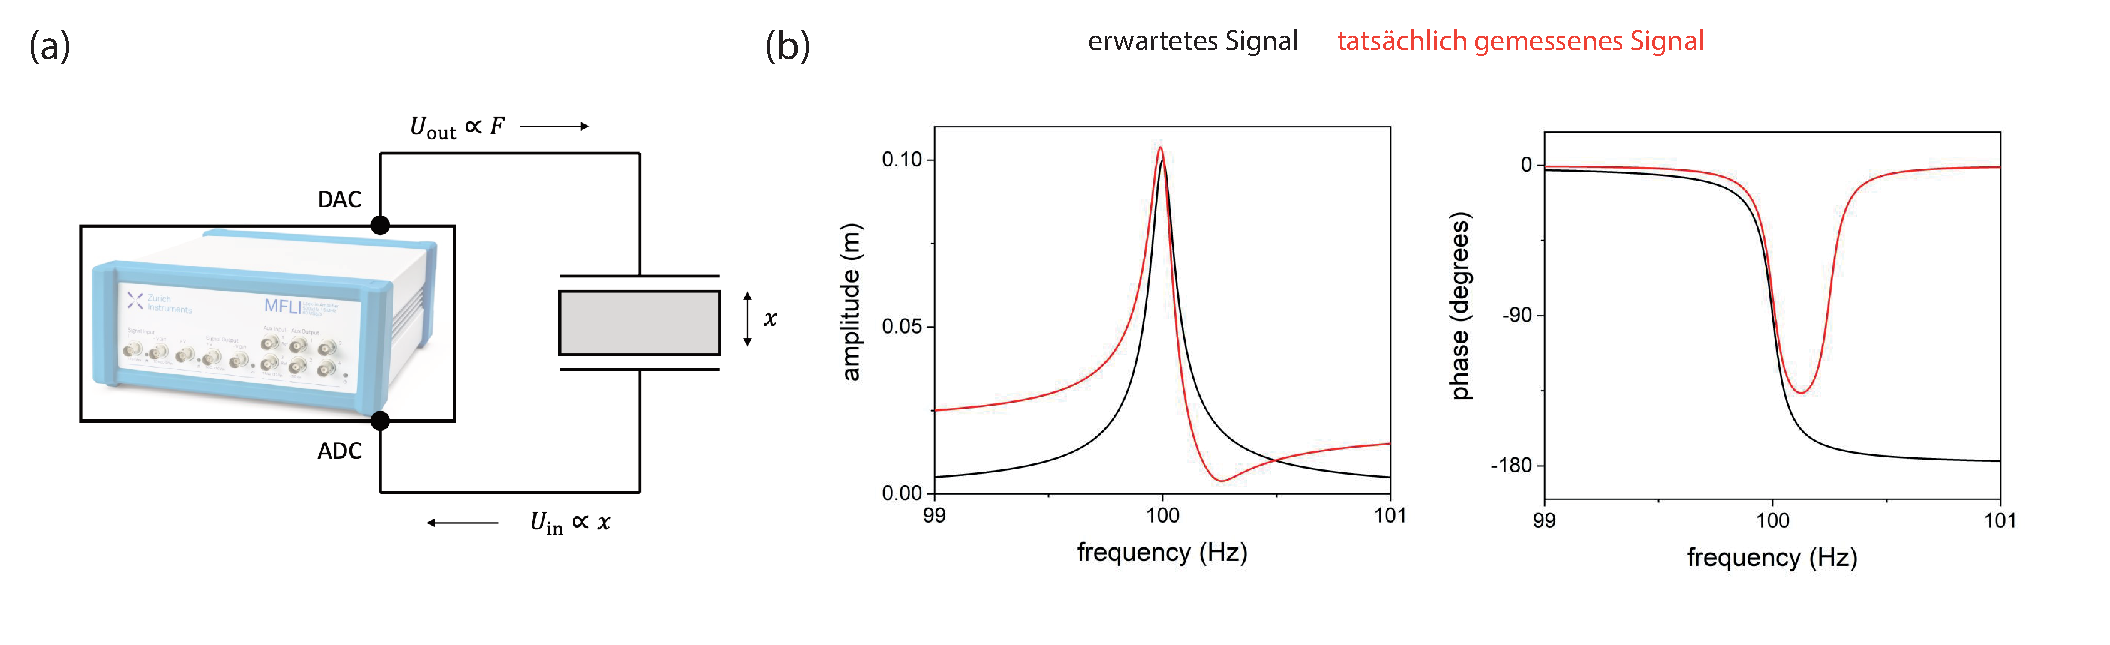
\includegraphics[width=0.9\textwidth]{Figures/modellundexperiment.pdf}
\caption{(a): Schematische Visualisierung des Versuchsaufbaus. (b): Erwartetes (schwarz) und tatsächlich gemessenes Signal (rot) für Amplitude (links) und Phase (rechts) von U$_{\mathrm{in}}$. }
\label{fig:oszillator}
\end{figure}

 Ein Modell kann allerdings niemals bewiesen, sondern immer nur widerlegt werden. Soll heissen: Auch wenn unser Experiment keine Lücken im Modell aufdeckt, könnte es immer noch ein anderes, alternatives Modell geben, das die gleiche Beobachtung erklären würde. Deckt unser Experiment hingegen eine Lücke auf, ist das Modell widerlegt worden und muss verworfen, beziehungsweise angepasst werden. Ein wichtiger Bestandteil dieses Prozesses, des Überprüfens eines Modells anhand eines Experiments, ist selbstverständlich die Analyse der gemessenen Daten. Kein Experiment ist komplett fehlerfrei, doch idealerweise sollten wir zwischen Fehlern des Modells und Fehlern des Experiments unterscheiden können. In diesem Kapitel wollen wir uns daher im Detail mit Messfehlern beschäftigen. 

\section{Messfehler}
\label{chap:fehler:sec:messfehler}

\begin{center}
\begin{tcolorbox}[enhanced,width=6in,center upper,
    fontupper=\large,drop fuzzy shadow southwest,
    colframe=blue!50!black,colback=blue!10]
Für dieses Unterkapitel ist ein Jupyter-Notebook verfügbar. Siehe \gitresource{Messfehler.ipynb}  
\end{tcolorbox}
\end{center}

\subsection{Was ist ein Messfehler?} % oder : Definition? 

Um zu verdeutlichen, was ein Messfehler ist, wollen wir zunächst ein einfaches Beispiel betrachten. Wir messen mit dem Beschleunigungssensor eines Smartphones die Erdbeschleunigung  \gls{gl:g}.\footnote{Dafür kann zum Beispiel die App Phyphox verwendet werden, Download möglich auf \href{https://phyphox.org}{phyphox.org}} Da der Wert der Erdbeschleunigung bereits mit sehr hoher Genauigkeit gemessen wurde,  erwarten wir schon vor der Messung ein bestimmtes Messergebnis, \gls{gl:xtilde}. Dieser erwartete Wert \gls{gl:xtilde} ist eine Abschätzung des tatsächlichen Werts von $g$, den wir (grundsätzlich) nicht kennen.  Während unserer ersten Messung von \gls{gl:g} erhalten wir nun einen Wert $x_1 \neq \Tilde{x}$. Der Abstand zwischen $x_1$ und \gls{gl:xtilde} ist der Fehler $e$ unserer Messung:
\begin{align}
\gls{gl:e} = \Tilde{x} - x_1\,.
\label{eq:messfehler}
\end{align}
Ein solcher Messfehler kann verschiedene Ursachen haben. Entweder kann bei der Messung selbst ein Fehler auftreten, z.B. durch  Ableseungenauigkeit, der Messung des falschen Parameters oder der ungenügenden Kalibration eines Messgerätes. Oder aber die Messung wird beeinflusst von (unbekannten) äusseren Faktoren wie z.B. Temperatur oder Luftfeuchtigkeit. \\

In jedem Fall gibt es bei einem Messvorgang für die gemessene Grösse einen tatsächlichen Wert, der - wie oben bereits erwähnt -  grundsätzlich unbekannt ist. Der erwartete Wert \gls{gl:xtilde} kann wie z.B. hier ein Literaturwert sein, oder ein theoretisch vorhergesagter Wert. Manchmal haben wir jedoch keine genaue Erwartung an den zu messenden Wert und können somit auch nicht direkt erkennen, ob unsere Messung stark vom erwarteten Wert abweicht. Somit müssen wir eine Möglichkeit finden, die Genauigkeit unserer Messung abzuschätzen und den Messfehler experimentell zu charakterisieren. 

%Alte Formulierung Laura: 
%Selbstverständlich kennen wir normalerweise den Erwartungswert \gls{gl:xtilde} der zu messenden Grösse nicht und können somit auch nicht den Fehler unserer Messung genau beziffern.\footnote{Ausnahmen sind Messungen von Naturkonstanten (z.B. \gls{gl:c}) oder anderen häufig verwendeten Werten (z.B. \gls{gl:g}), für die vertrauenswürdige Literaturwerte durch früheren Messungen vorliegen.}  Somit müssen wir eine Möglichkeit finden, die Genauigkeit unserer Messung abzuschätzen und den Messfehler experimentell zu charakterisieren. 

% Martin:
%Der erwartete Wert kann wie z.B. hier ein Literaturwert sein, oder ein theoretisch vorhergesagter Wert. Manchmal haben wir aber auch keine genaue Erwartung an den zu messenden Wert.
%In jedem Fall gibt es jedoch einen tatsächlichen Wert, der grundsätzlich unbekannt ist. 


\subsection{Systematische und zufällige Fehler}

Im Folgenden wollen wir zwischen systematischen und zufälligen Messfehlern unterscheiden.  Systematische Abweichungen sind konstante oder sich auf der Zeitskala unseres Experimentes nur sehr langsam ändernde Abweichungen des gemessenen Wertes vom tatsächlichen Wert. Solche systematischen Fehler können z.B. durch die falsche Kalibration einer Messapparatur zustande kommen. Sie können manchmal mittels einer Kontrollmessung einer bekannten Grösse in derselben Messapparatur aufgedeckt und eliminiert werden. Zufällige Fehler hingegen sind schnell fluktuierende Abweichungen, die bei jeder Durchführung des Experiments variieren und in der Regel nicht durch frühere Beobachtungen vorhergesagt werden können. Im Gegensatz zu systematischen Messfehlern sind zufällige Messfehler deutlich schwieriger auszuschliessen. Sie können lediglich reduziert, aber nicht vollständig eliminiert werden. Eine Messung, die zu Daten führt, die keine zufälligen Fehler zeigen, sollte misstrauisch machen.

\subsection{Statistische Analyse durch wiederholtes Messen} 

Der Messfehler lässt sich durch wiederholtes Messen $x_1$, $x_2$, $x_3$, ..., $x_N$  unserer Messgrösse statistisch analysieren. Aus unseren Messergebnissen, unserer sogenannten Stichprobe, können wir einen  \textbf{empirischen Mittelwert}
\begin{align}
\gls{gl:xoverline} = \frac{1}{N} \sum^N_{n = 1} x_n
\label{eq:empmean}
\end{align}
und eine \textbf{empirische Varianz}
\begin{align}
\gls{gl:deltax2}  = \frac{1}{N-1} \sum^N_{n = 1} \left( x_n - \gls{gl:xoverline} \right) ^2
\label{eq:empvar}
\end{align}
berechnen. Häufig wird auch die empirische Standardabweichung \gls{gl:deltax}, die Quadratwurzel der empirischen Varianz, verwendet. Sie ist somit ein Mass für systematische Fehler. Die \textbf{Präzision} einer Messung beschreibt die zufällige Verteilung der Messwerte um deren Mittelwert und ist somit ein Mass für zufällige Fehler. Beide Fehler lassen sich anschaulich in einem \textbf{Histogramm} darstellen, indem wir den Messbereich in gleich grosse ``Bins'' diskretisieren und die Messergebnisse innerhalb jedes Bins zählen (siehe Fig.~\ref{fig:messfehler1}).   \\

Kehren wir nun zu unserem anfänglichen Beispiel zurück. Wir führen $N$ Messungen von \gls{gl:g} durch und speichern die Ergebnisse in einem Numpy-Array $g$ ab. Ebenfalls speichern wir die zugehörigen Zeitpunkte $t$ der Messungen. In einem ersten Schritt visualisieren wir diese Daten in einem sehr einfachen Plot
\begin{lstlisting}[language = Python]
plt.plot(t, g)
\end{lstlisting}
und bestimmen den empirischen Mittelwert und die empirische Varianz der Stichprobe. Dies kann sowohl mithilfe der in \ref{eq:empmean} und \ref{eq:empvar} angegebenen Formeln   
\begin{lstlisting}[language = Python]
mean = np.sum(g)/N
var = np.sum((g-mean)**2)/(N-1)
\end{lstlisting}
oder aber durch Verwendung der Funktionen der numpy-Bibliothek. 
\begin{lstlisting}[language = Python]
mean = np.mean(g)
var = np.var(g)
\end{lstlisting}
geschehen. Hierbei ist zu beachten, dass die so berechnete Varianz nicht die empirische Varianz ist. Um die empirische Varianz zu erhalten muss die Varianz mit einem Faktor $\frac{N}{N-1}$ multipliziert werden.\\

Wir generieren nun unsere ``Bins'', um den Messbereich zu diskretisieren, und zählen die Messergebnisse pro Bin. Zur Auswahl der Breite der Bins ist die anfängliche Visualisierung der Daten hilfreich. Da die vertikale Auflösung unserer Messung ohnehin durch die Präzision unseres Messgerätes limitiert ist, wählen wir relativ breite Bins.  
\begin{lstlisting}[language = Python]
n_bins = 14+1 # Anzahl an Bins
bin_size = 0.005 # Breite des Bins 
bins = np.linspace(9.76, 9.76+bin_size*(n_bins-1), n_bins) 
# Initialisiere Numpy Array um Anzahl Messergebnisse pro Bin
# zu speichern
occurrence = np.zeros(n_bins)
offset = np.min(bins)//bin_size + 1
# Iteriere ueber alle Datenpunkte
# Bestimmte den Index des Bins, in den sie fallen
# Inkrementiere die Anzahl Ereignisse in diesem Bin um 1
for gx_i in gz:
    index = int(gx_i//bin_size-offset)
    occurrence[index] = occurrence[index] + 1
\end{lstlisting}
Nun können wir sehr einfach das Histogramm erstellen und den empirischen Mittelwert, die empirische Standardabweichung sowie den erwarteten Wert einzeichnen. Hierbei normalisieren wir unser Histogramm bereits entsprechend, um eine prozentuelle Wahrscheinlichkeit zu erhalten.\footnote{``Normalisieren'' bezeichnet die Multiplikation mit einem Faktor (in diesem Fall $A$), um der berechneten Grösse eine konkrete Bedeutung zuweisen zu können. In unserem Fall soll die Normierung erreichen, dass die Summe der Histogrammwerte 1 (oder 100 Prozent) ergibt.} 
\begin{lstlisting}[language = Python]
A =  N
g_theo = 9.78 
plt.bar(bins, occurrence/A, width = bin_size)
plt.vlines(g_theo, 0, np.max(occurrence)/A)
plt.vlines(mean, 0, np.max(occurrence)/A)
plt.vlines(mean + np.sqrt(var), 0, np.max(occurrence)/A)
plt.vlines(mean - np.sqrt(var), 0, np.max(occurrence)/A )
\end{lstlisting}
 Der von uns bestimmte Mittelwert weicht vom erwarteten Wert von  \gls{gl:g} ab, unsere Messung ist also nicht genau,  allerdings liegt der erwartete Wert noch innerhalb der empirischen Standardabweichung der Messung.
 % Hier fehlt noch ein abrundender Absatz

\begin{figure}[H]
\centering
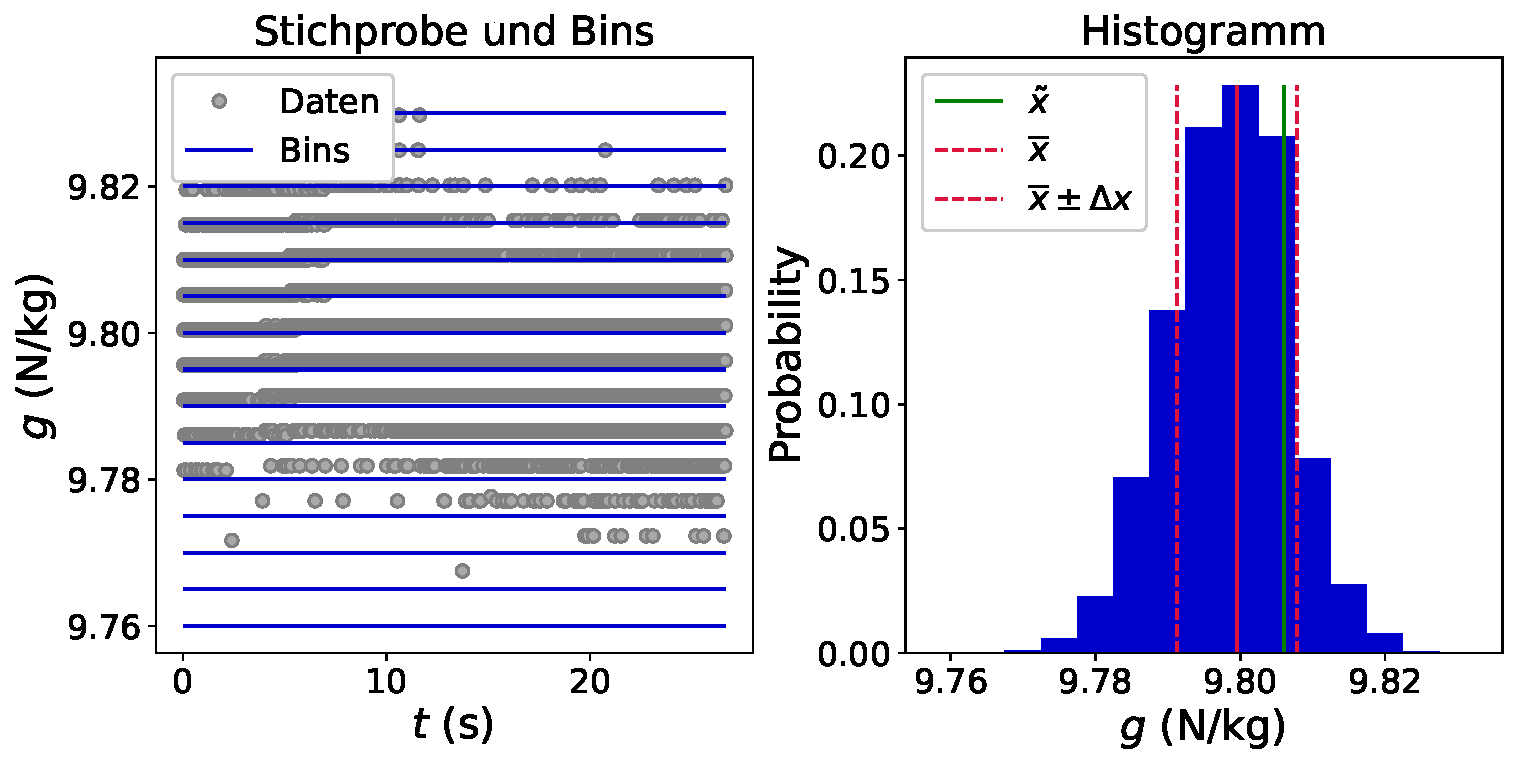
\includegraphics[width=0.9\textwidth]{Figures/messfehler1.pdf}
\caption{Statistische Analyse einer Messung von \gls{gl:g}. \textbf{Links:} Gemessene Datenpunkte (graue Punkte) als Funktion der Zeit $t$. Die Kanten der ``Bins'' sind als horizontale Linien indiziert. Aufgrund der limitierten vertikalen Auflösung der Messung arbeiten wir mit einer relativ geringen Anzahl von Bins.  \textbf{Rechts:} Das resultierende Histogramm der Stichprobe. Die Anzahl der Messergebniss pro Bin wurden für diese Darstellung bereits der Anzahl der Datenpunkte $N$ normalisiert, sodass die Summe aller Histogrammwerte 1 ergibt. Der erwartete Wert \gls{gl:xtilde} für die Erdbeschleunigung, sowie empirischer Mittelwert und empirische Standardabweichung sind eingezeichnet. }
\label{fig:messfehler1}
\end{figure}
%  Die Anzahl der Messergebniss pro Bins wurden für diese Darstellung bereits mit dem Produkt aus Anzahl der Datenpunkte $n$ und Bin-Breite normalisiert.

\section{Wahrscheinlichkeitsverteilungen}
\label{chap:fehler:sec:frequentistisch}

Im bisherigen Verlauf dieses Kapitels haben wir gelernt, wie wir zufällige Messfehler anhand der wiederholten Durchführung einer Messung charakterisieren können. Ein wichtiges Resultat dieser Analyse war hierbei das diskrete Histogramm der Ereignishäufigkeiten (siehe Fig.~\ref{fig:messfehler1}), die wir intuitiv als Wahrscheinlichkeiten, die entsprechenden Werte für unsere Messgrösse zu erhalten, interpretiert haben.  Im Folgenden wollen wir diesen Zusammenhang systematischer ergründen und hierzu den frequentistischen Wahrscheinlichkeitsbegriff und Wahrscheinlichkeitsverteilungen diskutieren.  Ein alternativer Ansatz zur Interpretation von Wahrscheinlichkeiten, die sogenannte Bayesische Datenanalyse, wird in Kapitel \ref{chap:estimation:sec:bayes} eingeführt. 

%erhaltene, diskrete Histogramm ist eine Abschätzung der kontinuierlichen Wahrscheinlichkeitsverteilung, die der Messung zugrunde liegt. Die Ergebnisse unserer Messung werden letztendlich von einer Wahrscheinlichkeitsverteilung beschrieben, eine Messgrösse ist eine Zufallsvariable und eine Messung ein Zufallsexperiment. Je grösser die Anzahl unserer Messpunkte ist und je besser unsere vertikale Auflösung ist, umso besser können wir die zugrundeliegende Verteilung beschreiben. Welche Verteilungsfunktion die Messung am besten beschreibt, hängt vom Experiment ab. Wichtige Verteilungen werden in Kapitel \ref{chap:pf} näher behandelt. In der Praxis finden wir sehr häufig normalverteilte Messergebnisse vor. Insbesondere liegt eine Normalverteilung immer dann vor, wenn der Messfehler tatsächlich vollkommen zufällig ist. Im Folgenden wollen wir daher auf die Normalverteilung näher eingehen.  \\

\subsection{Frequentistischer Wahrscheinlichkeitsbegriff}

Der frequentistische Wahrscheinlichkeitsbegriff entspricht der Definition, die wir intuitiv für unsere erste Analyse des Histogramms aus Fig.~\ref{fig:messfehler1} angenommen haben: Wir interpretieren den wiederholten Messvorgang einer experimentell zugänglichen Grösse als eine Reihe voneinander unabhängiger Zufallsexperimente und definieren die Wahrscheinlichkeit eines bestimmten Ergebnisses anhand der relativen Häufigkeit, mit der es in einer grossen Anzahl an Wiederholungen des Experiments auftritt. Im Grenzfall unendlich vieler Wiederholungen des Zufallsexperiment ist demnach die Wahrscheinlichkeit $P(A)$, dass ein bestimmtes Ereignis $A$ eintritt, mathematisch definiert als 
\begin{align}
P(A) = \frac{n_A}{n_S}\,
\label{eq:vl4-1}
\end{align}
wobei $n_S$ die Anzahl der möglichen Ergebnisse des Experiments ist und $n_A$ die Anzahl der Ergebnisse, die zu $A$ führen. Grundsätzlich gilt, dass die frequentistischen Wahrscheinlichkeiten $P$ umso besser aus den experimentellen Daten abgeschätzt werden können, je häufiger das Zufallsexperiment wiederholt wurde. Die heutige Popularität des frequentistischen Ansatzes ist somit zu grossen Teilen auf die gestiegenen technischen Standards und gesteigerten zur Verfügung stehenden Rechenleistungen zurückzuführen.  \\

Ein typisches Beispiel zur Veranschaulichung der frequentistischen Wahrscheinlichkeit ist der Würfelwurf. Hier ist die Anzahl der möglichen Ergebnisse $n_S=6$. Die Wahrscheinlichkeit, dass die Augenzahl grösser ist als 4 (d.h. $n_A = 2$) wäre folglich $P(A)=\frac{2}{6}=\frac{1}{3}$. Sofern eine ausreichend hohe Anzahl an Würfelwürfen durchgeführt, sollte somit ungefähr in jeder dritten Messung eine Augenzahl, die grösser ist als 4, auftreten. \\

Da ein mögliches Ergebnis $A$ immer eine Teilmenge der Gesamtmenge aller möglichen Ergebnisse $S$ des Experiments darstellt, gilt  stets
\begin{align}
A \subseteq S:  \quad 0 \leq P ( A ) \leq 1
\end{align}
und zudem
\begin{align}
P(S) =  P(A) + P(\overline{A}) =  1,
\end{align}
wobei $P(\overline{A})$ die Wahrscheinlichkeit ist, dass Ergebnis $A$ \textit{nicht} eintritt. \\

Häufig sind wir gleichzeitig an mehreren möglichen Ergebnissen, z.B. $A$ und $B$, des Experiments interessiert und wollen zusätzlich zu deren individuellen frequentistischen Wahrscheinlichkeiten, $P(A)$ und $P(B)$, auch kompliziertere Wahrscheinlichkeiten berechnen, die beide Ergebnisse betreffen. Zu diesem Zweck ist es hilfreich, sogenannte Venn-Diagramme (auch: Mengendiagramme) zu verwenden, die den Grad an Überlapp der Teilmengen mehrerer Ergebnisse und folglich deren Schnittmengen ($A\cap B$), Vereinigungsmengen ($A \cup B$) sowie Differenzmengen ($A\setminus B $, $B \setminus A$)  graphisch darstellen können. In unserem anfänglichen Beispiel des Würfels könnten wir etwa zusätzlich zum Ergebnis $A:$\glqq Die Augenzahl ist grösser als 4\grqq auch das Ergebnis $B:$\glqq Die Augenzahl ist 6\grqq betrachten. Im entsprechenden Venn-Diagramm überlappen die Teilmengen dieser Ergebnisse, da sie gleichzeitig eintreten können - die Augenzahl ist schliesslich grösser als 4, wenn sie 6 beträgt. 

\begin{figure}[H]
\centering
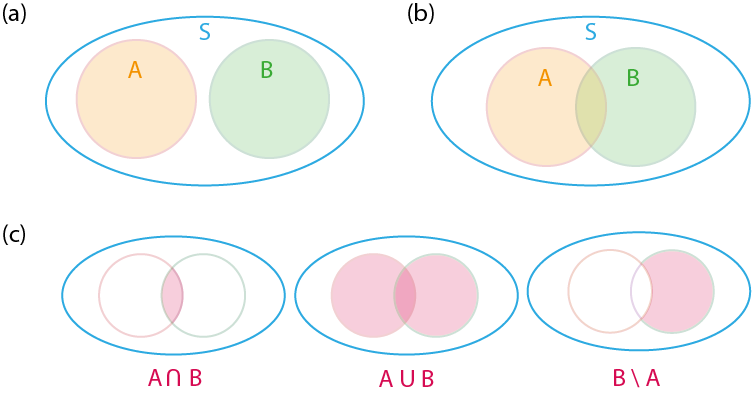
\includegraphics[width=0.6\textwidth]{Figures/venndiagramm.png}
\caption{Venn-Diagramme zur Veranschaulichung von Frequentistischen Wahrscheinlichkeiten. Die Ergebnisse $A$ und $B$ sind Teilmengen der Gesamtmenge $S$ aller möglichen Ergebnisse des Experiments. \textbf{(a)} Wenn die Ergebnisse $A$ und $B$ nicht gleichzeitig eintreten können, überlappen ihre Teilmengen im Venn-Diagramm nicht. \textbf{(b)} Wenn die Ergebnisse $A$ und $B$ gleichzeitig eintreten können, gibt es einen gewissen Überlapp zwischen ihren Teilmengen. \textbf{(b)} Venn-Diagramme sind hilfreich, um Schnittmengen, Vereinigungsmengen und Differenzmengen darzustellen.  }
\label{fig:venn}
\end{figure}

 Die Wahrscheinlichkeit $P(A \cup B)$, dass entweder Ereignis $A$ oder Ereignis $B$ eintritt, ist
\begin{align}
P(A \cup B) = P(A) + P(B) - P(A\cap B),
\label{eq:kombp}
\end{align}
wobei wir die Wahrscheinlichkeit $P(A\cap B)$ des gleichzeitigen Auftretens beider Ergebnisse subtrahieren müssen, um im Fall von überlappenden Ergebnismengen die entsprechende Fläche des Venn-Diagramms nicht doppelt zu zählen. Weiterhin ist häufig die  konditionelle  (auch: bedingte) Wahrscheinlichkeit $P(A|B)$, dass Ergebnis $A$ eintritt, wenn $B$ eintritt, von Interesse. Sie ist gegeben als
\begin{align}
P ( A | B ) = \frac{P ( A \cap B )}{P ( B )}.
\label{eq:kondp}
\end{align}
  Da $P(A \cap B) = P(B \cap A)$ können wir folgend aus Gleichung \ref{eq:kondp} den  Zusammenhang
\begin{align}
P ( A \cap B ) = P ( A | B ) P ( B ) = P ( B | A ) P ( A )\
\label{eq:bayespre}
\end{align}
 zwischen $P(A|B)$ und $P(B|A)$ herstellen. Aus diesem folgt schliesslich der sogennannte Satz von Bayes,
\begin{align}
P ( B | A ) = \frac{P ( A | B) P ( B )}{P ( A )}. 
\label{eq:bayes}
\end{align}

Die bisherige Betrachtung ist unabhängig davon, ob ein kausaler Zusammenhang zwischen $A$ und $B$ herrscht, korrekt. Falls kein solcher Zusammenhang besteht, d.h. $A$ und $B$ vollkommen unabhängig sind, entsprechen die bedingten Wahrscheinlichkeiten einfach den individuellen Wahrscheinlichkeiten der Ergebnisse, d.h.  
\begin{align}
P ( A | B ) = P(A). 
\end{align}
Weiterhin gilt dann
\begin{align}
 P ( A \cap B ) = P ( A ) P ( B ).
\end{align}

\subsection{Wahrscheinlichkeitsverteilungen - Grundlegende Charakteristiken}

Dem frequentistischen Wahrscheinlichkeitsbegriff folgend stellt das aus den Ergebnissen der wiederholten Messung der Zufallsvariablen erhaltene Histogramm (siehe Fig.~\ref{fig:messfehler1}) in einer diskreten Form die Wahrscheinlichkeiten als Funktion des Messwertes da. Es bildet somit, sofern zum Einen eine ausreichend hohe Anzahl an Wiederholungen durchgeführt wurde und zum Anderen sowohl die vertikale als auch horizontalen Auflösungen der Messung es zulassen, näherungsweise die zugrundeliegende (kontinuierliche) Wahrscheinlichkeitsverteilung der Messgrösse ab. Im Folgenden werden wir zunächst einige grundlegende Charakteristiken von Wahrscheinlichkeitsverteilungen definieren und dann auf einige relevante, konkrete Wahrscheinlichkeitsverteilungen eingehen. \\ 

Eine Wahrscheinlichkeitsverteilung ist eine positive und normierte Funktion, die die Verteilung der Wahrscheinlichkeit einer Zufallsvariablen $x$ beschreibt.  Falls die Zufallsvariable nur diskrete Werte annehmen kann, spricht man von einer sogenannten  \textbf{Probability Mass Function} (PMF), die jedem möglichen, diskreten Wert $x_n$ der Zufallsvariable eine Wahrscheinlichkeit $P(x_n)$ zuordnet. Es gilt 
\begin{align}
0 \leq P(x_n) \leq 1,
\end{align}
sowie
\begin{align}
\sum_n P(x_n) = 1.
\end{align}
Im Falle einer kontunierlichen Zufallsvariablen $x$ sprechen wir von einer  \textbf{Probability Density Function} (PDF) (zu deutsch: Wahrscheinlichkeitsdichtefunktion) $f(x)$ die
\begin{align}
0 \leq  f(x) 
\end{align}
und
\begin{align}
\int_{-\infty}^{\infty} f(x) = 1
\end{align}
erfüllt. Während im diskreten Fall die Wahrscheinlichkeit für das Auftreten eines bestimmten Wertes $x_n$ direkt aus der PMF abgelesen werden kann, entspricht im kontinuierlichen Fall $f(x)$ nicht direkt der Wahrscheinlichkeit für das Auftreten eines Wertes $x$. Stattdessen kann die Wahrscheinlichkeit dafür, dass das Ergebnis $x$ in in einem Intervall zwischen $a$ und $b$ liegt, durch Integration der PDF als  
\begin{align}
P(a\leq x \leq b) = \int_a^bf(x)dx
\end{align}
erhalten werden. \\

In Tabelle \ref{tab:pdfs} sind einige der wichtigsten Kennzahlen von Wahrscheinlichkeitsdichtefunktionen aufgelistet.

\begin{longtable}{p{3cm}|p{6cm}|p{5cm}}
\caption{Auflistung einiger wichtiger Kennzahlen von Wahrscheinlichkeitsdichtefunktionen.} \\
\textbf{Name und Variable} & \textbf{Formel} & \textbf{Bedeutung} \\ \hline \hline
Modus \gls{gl:xmode} & \begin{align}
\gls{gl:xmode}: \frac{d f ( x )}{dx}\bigg|_{\gls{gl:xmode}} = 0 
\end{align} & Der Wert von $x$, bei dem die Verteilung ihr Maximum erreicht. Die hier angegebene Formel zur Berechnung kann für eine PDF mit einem einzigen Maximum verwendet werden. \\ \hline 
Median $x_{\mathrm{median}}$ & \begin{align}
\frac{1}{2} = \int_{-\infty}^{x_{\mathrm{median}}} f ( x ) dx\
\end{align}  & Die Mitte der Verteilung. Der Median wird häufig bei der Darstellung von sozioökonomischen Daten verwendet, etwa zur Angabe des durchschnittlichen Gehalts einer Gesellschaft. \\ \hline
Halbwertsbreite  \gls{gl:FWHM} & \begin{align} \begin{split}
f ( a ) = f ( b ) = \frac{1}{2} f (\gls{gl:xmode} ) \\  \gls{gl:FWHM} = b - a\,.
\end{split} \end{align} & Charakterisiert die Breite der Verteilung beim halben Wert ihres Maximalwertes. \\ \hline
Erwartungswert \gls{gl:mu} & \begin{align} \begin{split} \mu = E(x) \\ = \int_{-\infty}^{+\infty} xf(x)dx \end{split} \end{align} & Die Zahl, die die Zufallsvariable $x$ im Mittel annimmt. Häufig wird der Erwartungswert auch als Mittelwert bezeichnet. \\ \hline
Varianz \gls{gl:var} &   \begin{align} \begin{split} \gls{gl:var} = E((x-\gls{gl:mu})^2) \\ = \int_{-\infty}^{+\infty} (x-\gls{gl:mu})^2f(x)dx \end{split} \end{align} &  Die mittlere quadratische Abweichung der Zufallsvariablen $x$ von ihrem Erwartungswert. \\ \hline
Standardabweichung \gls{gl:sigma} & \begin{align} \gls{gl:sigma} = \sqrt{\gls{gl:var}} \end{align} 
\label{tab:pdfs}
\end{longtable}

Zusätzlich zu diesen Charakteristika lassen sich für viele PDF sogenannte Momente berechnen. Das $m$-te Moment $M_m$ einer Wahrscheinlichkeitsverteilung $f(x)$ ist definiert als
\begin{align}
M_m = \int_{-\infty}^{+\infty} x^mf(x)dx.
\end{align}
Das 0-te Moment
\begin{align}
M_0 = \int_{-\infty}^{+\infty} f(x)dx = 1
\end{align}
entspricht somit der Normierungsbedingung der Wahrscheinlichkeitsverteilung, während das 1-te Moment
\begin{align}
M_1 = \int_{-\infty}^{+\infty} xf(x)dx = E(x)
\end{align}
ihren Mittelwert liefert. \\

Ebenfalls ist das $m$-te zentrale Moment einer Wahrscheinlichkeitsverteilung definiert als
\begin{align}
\Tilde{M}_m = \langle ( x - M_1 )^m \rangle\,.
\end{align}
Damit ist die Varianz einer PDF gegeben durch das zweite zentrale Moment:
\begin{align}
\sigma^2 = \langle ( x - M_1)^2 \rangle = \langle x^2 \rangle - \langle x \rangle^2 = M_2 - M_1^2\,.
\end{align}
Das dritte zentrale Moment quantifiziert die  Schiefe und das vierte zentrale Moment die Wölbung der PDF. Es ist hilfreich, die momenterzeugende Funktion zu definieren und unter Verwendung der Taylorreihe von $\exp ( \zeta x )$ zu formulieren
\begin{align}
\begin{split}
M ( \zeta ) = \int_{-\infty}^{+\infty} \exp ( \zeta x ) f ( x ) dx \\ 
= \int_{-\infty}^{+\infty} \left( 1 + \zeta x + \frac{ \zeta^2 x^2 }{ 2! } + \cdots \right) f ( x ) dx\\
= M_0 + \zeta M_1 + \frac{ \zeta^2 }{ 2! } M_2 + \cdots .
\end{split}
\end{align}
Höhere Momente $m \geq 1$ können iterativ aus der Ableitung der momenterzeugenden Funktion berechnet werden:
\begin{align}
M_m = \frac{ \partial^m M ( \zeta ) }{ \partial \zeta^m} \bigg|_{\zeta = 0}\,.
\end{align}\\

Darüber hinaus ist es hilfreich, die charakteristische Funktion $\phi(\nu)$
\begin{align}
\phi(\nu) = \int_{-\infty}^{+\infty} \exp ( \mathrm{i} \nu x) f ( x ) dx.
\label{eq:charakteristischefunktion}
\end{align}
 einer Wahrscheinlichkeitsverteilung $f(x)$ zu definieren, wobei $\mathrm{i}=\sqrt{-1}$ die imaginäre Einheit ist. Die charakteristische Funktion ist die inverse Fouriertransformierte der Wahrscheinlichkeitsverteilung. Die Fourier-Transformation werden wir in Kapitel \ref{ch:spectral} zur Spektralanalyse genauer kennenlernen.  Indem wir die Exponentialfunktion erweitern, können wir die charakteristische Funktion als Funktion der Momente der PDF ausdrücken:
\begin{align}
\begin{split}
\phi ( \nu ) & = \int_{-\infty}^{+\infty} \left( 1 + \mathrm{i} \nu x + \frac{ 1 }{ 2! } ( \mathrm{i} \nu )^2 x^2 + \frac{ 1 }{ 3! } ( \mathrm{i} \nu )^3 x^3 + \cdots \right) f ( x ) dx\\
& = 1 + \mathrm{i} \nu M_1 + \frac{ 1 }{ 2 ! } ( \mathrm{i} \nu )^2 M_2 + \frac{ 1 }{ 3! } ( \mathrm{i} \nu )^3 M_3 + \cdots\,.
\end{split}
\end{align}
Ausserdem können wir wir die Wahrscheinlichkeitsverteilung $f(x)$ durch Fouriertransformation von $\phi(\nu)$ berechnen:
\begin{align}
f ( x ) = \frac{ 1 }{ 2 \pi } \int_{-\infty}^{+\infty} \exp ( -\mathrm{i} \nu x ) \phi ( \nu ) d \nu\,.
\end{align}
Die Kombination dieser beiden Ergebnisse ergibt:
\begin{align}
f ( x ) = \frac{ 1 }{ 2 \pi } \int_{-\infty}^{+\infty} \exp ( -\mathrm{i} \nu x ) \left( 1 + \mathrm{i} \nu M_1 + \frac{ 1 }{ 2 ! } ( \mathrm{i} \nu )^2 M_2 + \frac{ 1 }{ 3! } ( \mathrm{i} \nu )^3 M_3 + \cdots \right)  d \nu\,.
\end{align}

\subsection{Die Normalverteilung}

In der Praxis finden wir sehr häufig normalverteilte Messergebnisse vor. Insbesondere liegt eine Normalverteilung immer dann vor, wenn der Messfehler  aus der additiven Überlagerung zahlreicher unabhängiger, zufälliger Ereignisse resultiert und somit selbst tatsächlich vollkommen zufällig ist.  Der Grund hierfür ist der sogenannte \textbf{zentrale Grenzwertsatz}:\\

\begin{center}
\begin{tcolorbox}[enhanced,width=6in,drop fuzzy shadow southwest,
    colframe=red!50!black,colback=red!05]
   Die Summe vieler (identisch verteilter)
Zufallsvariablen ist eine normalverteilte
Zufallsvariable. \\

\underline{Beispiel}: Während die Augenzahl beim Wurf eines einzelnen Würfels gleichverteilt ist, ist die Summe der Augenzahlen mehrerer Würfel normalverteilt.
\end{tcolorbox}
\end{center}

Die Normalverteilung wird daher häufig als Modell für die Wahrscheinlichkeitsverteilung von Messdaten angenommen, sofern keine Kenntnis über das Vorhandensein einer anderen, physikalisch motivierten Verteilung besteht. Sie wird durch den Erwartungswert \gls{gl:mu} und die Standardabweichung (die Quadratwurzel der Varianz) \gls{gl:sigma} $= \sqrt{ \gls{gl:var}}$ parametrisiert.
\begin{align}
f( x, \gls{gl:mu}, \gls{gl:sigma} ) = \frac{ 1 }{ \sigma \sqrt{ 2 \pi }} \exp{ \left( - \frac{ \left( x - \gls{gl:mu} \right)^2}{2 \sigma ^2} \right) }\,.
\label{eq:normalverteilung}
\end{align}
 Die Standardabweichung gibt hierbei das Gewicht der \gls{gl:PDF} um den Erwartungswert an: Ein Messergebnis liegt mit 68\,\% Wahrscheinlichkeit innerhalb des Intervalls $\left[ \gls{gl:mu} - \gls{gl:sigma} \text{, } \gls{gl:mu} + \gls{gl:sigma} \right]$. Je breiter das Intervall, desto mehr Gewicht, d.h. umso wahrscheinlicher ist es, ein Messergebnis im Intervall zu finden:
\begin{align}
\begin{split}
1\sigma & \rightarrow 68\,\% \\
2\sigma & \rightarrow 95\,\% \\ 
3\sigma & \rightarrow 99.7\,\% \\ 
& \cdots \\
5\sigma & \rightarrow 99.99994\,\%
\end{split}
\end{align}

Selbstverständlich sind die Parameter (\gls{gl:mu}, \gls{gl:sigma}) der Normalverteilung, die einer gemessenen Stichprobe zugrunde liegt, zunächst unbekannt und müssen anhand der experimentell gemessenen Daten möglichst gut abgeschätzt werden. Wir wollen dafür den Erwartungswert $E(x) =\gls{gl:mu}$ mit dem empirischen Mittelwert \gls{gl:xoverline}  und die Standardabweichung  \gls{gl:sigma} mit der empirischen Standardabweichung \gls{gl:deltax} annähern. Aber dürfen wir das?  \\ 

Um zu überprüfen, ob der empirische Mittelwert und die emprische Varianz gute Schätzwerte für den tatsächlichen Erwartungswert und die tatsächliche Varianz sind, bilden wir deren Erwartungswerte, $E(\Bar{x})$ und $E(\gls{gl:deltax2})$.  Zunächst berechnen wir den Erwartungswert des empirischen Mittelwertes:
\begin{align}
E(\Bar{x}) = E \left( \frac{1}{N} \sum_{n = 1}^N x_n \right) = \frac{1}{N} \sum_{n = 1}^N E(x_n)\,.
\end{align}
wobei wir verwendet haben, dass der Erwartungswert linear ist und somit für unabhängige Zufallsvariablen $X$, $Y$ sowie Konstanten $a$, $b$ gilt:
\begin{align}
\begin{split}
E(a) &= a\\
E(aX) &= a E(X)\\
E(aX + b) &= a E(X) + b\\
E(aX + bY) &= a E(X) + b E(Y)\,.
\end{split}
\end{align}
Wenn wir nun weiterhin beachten, dass jede einzelne Messung der Zufallsvariable den gleichen Erwartungswert besitzt wie die Zufallsvariable selbst (d.h. $E(x_n) = E(x)$) erhalten wir
\begin{align}
E(\Bar{x}) = \frac{1}{N} \sum_{n = 1}^N E(x_n)= \frac{1}{N} \sum_{n = 1}^N E(x) = \frac{1}{N} N E(x) = E(x)\,.
\end{align}
Der Erwartungswert des Mittelwertes entspricht also tatsächlich dem Erwartungswert der Zufallsvariablen. Der aus den Stichproben erhaltene empirische Mittelwert ist somit in der Tat ein guter Schätzwert für den tatsächlichen Erwartungswert:
\begin{align}
\mu \approx \overline{x} = \frac{1}{N} \sum^N_{n = 1} x_n\,,
\end{align}

Wir gehen nun analog vor für die Varianz und berechnen ihren Erwartungswert. Hierfür verwenden wir den Zusammenhang
\begin{align}
\text{var}(x) = E(x^2) - E(x)^2 \rightarrow E(x^2) = \text{var}(x) + E(x)^2
\end{align}
sowie
\begin{align}
\text{var}(\bar{x}) = \frac{\text{var}(x)}{N} 
\end{align}
und können damit folgende Umformung vornehmen: 
\begin{align}
\begin{split}
E(\gls{gl:deltax2}) &= E \left( \frac{1}{N-1} \sum_{n=1}^N ( \bar{x} - x_n )^2 \right)\\
&= E \left( \frac{1}{N-1} \sum_{n=1}^N ( \bar{x}^2 - 2 \bar{x} x_n + x_n^2 ) \right)\\
&= E \left( \frac{1}{N-1} \left( \sum_{n=1}^N \bar{x}^2 - 2 \sum_{n=1}^N \bar{x} x_n + \sum_{n=1}^N x_n^2 \right) \right)\\
&= E \left( \frac{1}{N-1} \left( N \bar{x}^2 - 2 \bar{x} \sum_{n=1}^N x_n + \sum_{n=1}^N x_n^2 \right) \right)\\
& = E \left( \frac{1}{N-1} \left( N \bar{x}^2 - 2 N \bar{x}^2 + \sum_{n=1}^N x_n^2 \right) \right)\\
&= E \biggl( \frac{1}{N-1} \biggl( \sum_{n=1}^N x_n^2 - N \bar{x}^2 \biggr) \biggr)\\
&= \frac{1}{N-1} \left( \sum_{n=1}^N E(x_n^2) - N E(\bar{x}^2) \right)\\
& = \frac{1}{N-1} \left( \sum_{n=1}^N (\text{var}(x) + E(x)^2 - N E(\bar{x}^2) \right)\\
& = \frac{1}{N-1} \left( \sum_{n=1}^N (\text{var}(x) + E(x)^2) - N \left( \frac{\text{var}(x)}{N} + E(\bar{x})^2 \right) \right)\\
&= \frac{1}{N-1} ( N \text{var}(x) - N E(x)^2 - \text{var}(x) + N E(\bar{x})^2 )\\
&= \frac{1}{N-1} (\text{var}(x) (N-1) - N E(x)^2 + N E(x)^2 ) \\
&= \frac{1}{N-1} \text{var}(x) (N-1) \\
&= \text{var}(x)\,.
\end{split}
\end{align}
Somit ist auch die empirische Standardabweichung ein guter Schätzwert der Standardabweichung.
\begin{align}
\gls{gl:sigma} \approx \gls{gl:deltax} = \sqrt{\frac{1}{N-1} \sum^N_{n = 1} \left( x_n - \gls{gl:xoverline} \right)^2}\,.
\end{align}

Jetzt, da wir die empirische Standardabweichung und Varianz als gute Schätzwerte für Erwartungswert und Varianz identifiziert haben, wollen wir zu unserem Datensatz an Messdaten für \gls{gl:g} aus Abschnitt \ref{chap:messfehler:sec:messfehler} zurückkehren. Zunächst wollen wir überprüfen, ob die von uns gemessenen Daten  tatsächlich einer Normalverteilung folgen. Wir berechnen, welcher Anteil unserer Messwerte im $1\sigma$-Intervall liegt und vergleichen das Resultat mit dem für die Normalverteilung erwarteten Wert.
\begin{lstlisting}[language = Python]
n_sigma = 0
width = 1
# Iteriere durch alle Bins und addiere ihre Werte auf, wenn sie im entsprechenden Intervall liegen
i = 0
for b in bins:
    if (b >= (mean - np.sqrt(var) * width)) and (b <= (mean + np.sqrt(var) * width)):
        n_sigma = n_sigma + occurrence[i]
    i = i + 1
print('Occurences within the {:d}-sigma-interval: {:0.1f}%'.format(width,n_sigma/N*100))
\end{lstlisting}
Wir finden, dass 64.7 Prozent unserer Messung im $1\sigma $ Intervall liegen, was sehr nah am erwarteteten Wert für die Gaussverteilug liegt. Auch entsprechende Berechnungen für die grösseren Intervalle liefern Ergebnisse, die sehr ähnlich zu den erwarteten Werten sind. Unsere Stichprobe scheint tatsächlich normalverteilt zu sein. \\ 

In einem weiteren Schritt simulieren wir nun unter der Annahme einer Normalverteilung und unter Verwendung unserer empirisch gemessenen Mittelwerts und Standardabweichung als Schätzungen der Parameter einen Datensatz mit höherer vertikaler Auflösung. Hierzu verwenden wir das random-Modul in Python:
\begin{lstlisting}[language = Python]
g_sim = np.random.normal(mean, np.sqrt(var), N)
\end{lstlisting}
Wir analysieren die so erhaltenen Werte analog zu unserem ursprünglichen Datensatz, verwenden nun allerdings deutlich schmälere Bins und normalisieren die erhaltenen Ereignishäufigkeiten nicht nur mit der Anzahl $N$ der Messungen, sondern ebenfalls mit der Bin-Breite, um eine Wahrscheinlichkeitsdichte (\textit{Probability Density})  zu erhalten.  Ebenfalls zeichnen wir die zugehörige Normalverteilung als Graph ein (siehe Figur \ref{fig:messfehler2}). Dieser Vergleich versinnbildlicht, dass eine Messung mit ausreichender Anzahl Datenpunkten und entsprechender Auflösung die zugrundeliegende Wahrscheinlichkeitsverteilung sehr gut abbilden kann.

\begin{figure}[H]
\centering
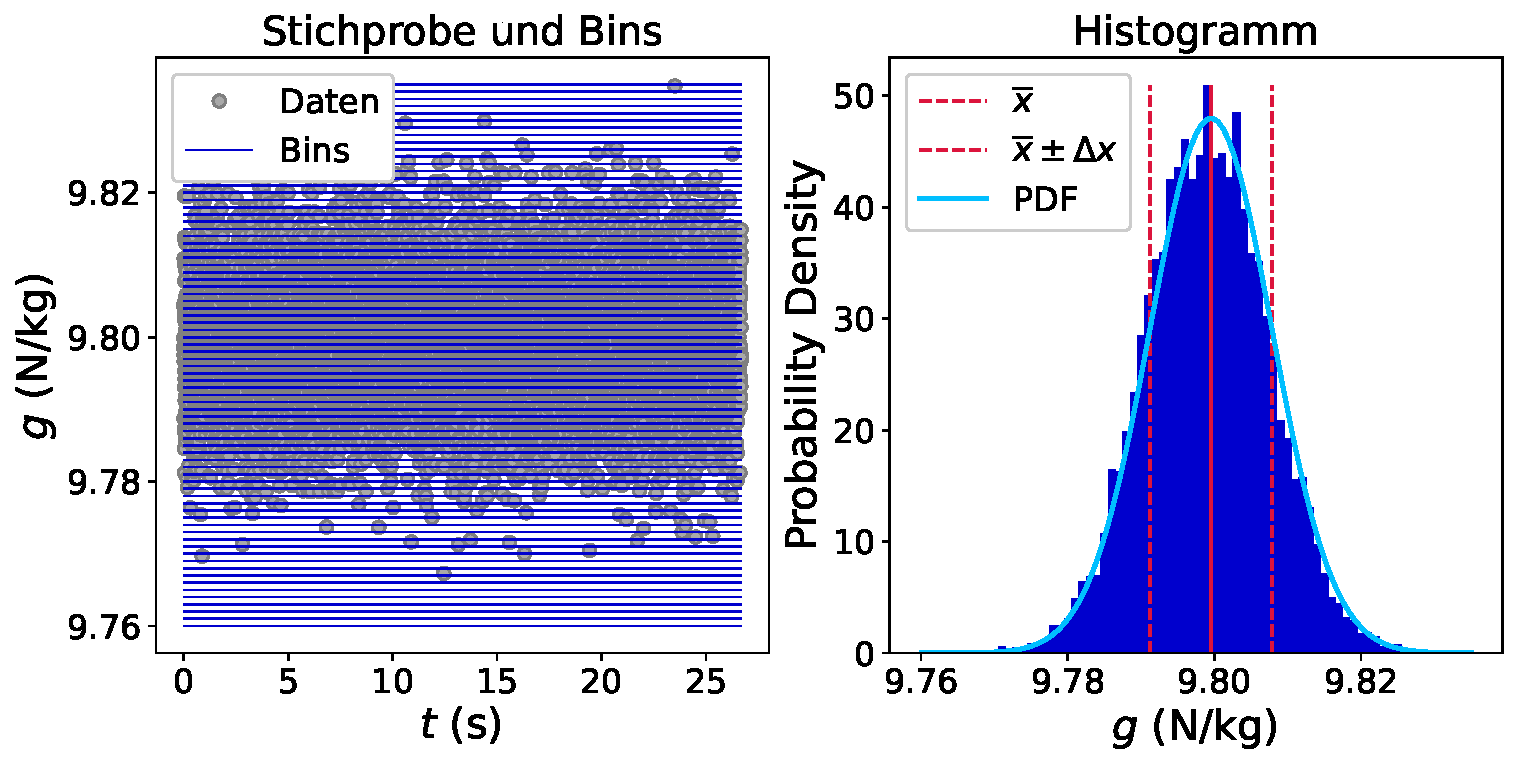
\includegraphics[width=0.9\textwidth]{Figures/messfehler2.pdf}
\caption{Statistische Analyse einer simulierten Messung von \gls{gl:g} mit höherer Auflösung. \textbf{Links:} Auftragung der gemessenen Datenpunkte (graue Punkte) gegen die Zeit $t$. Die Kanten der ``Bins'' sind als horizontale Linien indiziert.   \textbf{Rechts:} Das resultierende Histogramm der Stichprobe. Die Anzahl der Messergebniss pro Bins wurden für diese Darstellung bereits mit dem Produkt aus Anzahl der Datenpunkte $n$ und Bin-Breite normalisiert, um eine Wahrscheinlichkeitsdichte zu erhalten. Der empirische Mittelwert und die empirische Standardabweichung (rote Linien), sowie die aus diesen erhaltene Normalverteilung (blaue Linie) sind eingezeichnet.}
\label{fig:messfehler2}
\end{figure}


\subsection{Binomial- und Poissonverteilung}
Die Binomialverteilung ist eine der wichtigsten, diskreten Wahrscheinlichkeitsverteilungen. Sie liegt immer dann vor, wenn eine Serie von $n$ unabhängigen und gleichartigen Versuchen zur Messung einer Zufallsvariablen mit lediglich zwei möglichen Ergebnissen, $d$ und $u$, durchgeführt wird. Ein typisches Alltagsbeispiel für eine Binomialverteilung wäre etwa der Münzwurf, ein Beispiel der statistischen Physik die Besetzung eines Zustandes mit einer Reihe von Spins, die sich entweder in einem \glqq up\grqq{} (d.h. $S_z = +\frac{1}{2}\hbar$) oder \glqq down\grqq{} (d.h. $S_z = -\frac{1}{2}\hbar$) Zustand befinden können. Die Wahrscheinlichkeiten für die beiden Ergebnisse sind in jeder Durchführung des Versuchs identisch und  
\begin{align}
P(u) = p,
\end{align}
\begin{align}
P(d) = q = 1-p.
\end{align}
Die Binomialverteilung 
\begin{align}
B(k|p, n) = \frac{ n! }{ k! (n - k)! }p^k (1-p)^{n-k}
\end{align}
gibt die Wahrscheinlichkeit $B(k|p, n)$ dafür an, dass in $n$ Versuchen $k$-mal das Ergebnis $u$ auftritt. Sie setzt sich zusammen aus der der Wahrscheinlichkeit $p^k (1-p)^{n-k}$ für das Auftreten der $k$ Ereignisse in einer bestimmten Reihenfolge und dem Binomialkoeffizienten
\begin{align}
\begin{pmatrix} n\\ k \end{pmatrix} \equiv \frac{ n! }{ k! (n - k)! },
\end{align}
der angibt, auf wie viele verschiedene Arten man aus einer Menge von $n$ Objekten $k$ Objekte auswählen kann. Als Wahrscheinlichkeitsverteilung muss dies natürlich normiert sein, sodass wir als 0-tes Moment 
\begin{align}
M_0 = \sum_{k = 0}^n \begin{pmatrix} n\\ k \end{pmatrix} p^k q^{n-k} = 1
\end{align}
erhalten.  Wir wollen nun die höheren Momente ($m \geq 1$) mithilfe der Ableitung der Momenterzeugenden Funktion
\begin{align}
M_m = \frac{ \partial^m M (\zeta) }{ \partial \zeta^m} \bigg|_{\zeta = 0}
\end{align}
berechnen. Wir berechnen die Ableitung als
\begin{align}
\begin{split}
\frac{ \partial M_m }{ \partial p } &= \frac{ \partial }{ \partial p } \left( \sum_{k = 0}^n k^m \begin{pmatrix} n \\ k \end{pmatrix} p^k (1 - p)^{n-k} \right)\\
&= \sum_{k = 0}^n k^{m + 1} \begin{pmatrix} n \\ k \end{pmatrix} p^{k - 1} (1 - p)^{n - k} - \sum_{k = 0}^n k^m (n - k) \begin{pmatrix} n \\ k \end{pmatrix} p^k (1 - p)^{n - k - 1}\\
&= \frac{1}{p} \sum_{k = 0}^n k^{m + 1} \begin{pmatrix} n \\ k \end{pmatrix} p^k q^{n - k} - \frac{n}{q} \sum_{k = 0}^n k^m \begin{pmatrix} n \\ k \end{pmatrix} p^k q^{n - k} + \frac{1}{q} \sum_{k = 0}^n k^{m + 1} \begin{pmatrix} n \\ k \end{pmatrix} p^k q^{n - k}\\
&= \frac{1}{p} M_{m + 1} - \frac{n}{1} M_m + \frac{1}{q} M_{m + 1}.
\end{split}
\end{align}
und können somit die höheren Momente mittels 
\begin{align}
M_{m + 1} = n p M_m + p q \frac{ \partial M_m }{ \partial p } 
\end{align}
berechnen. Wir erhalten somit das erste Moment, den Mittelwert der Binomialverteilung, als 
\begin{align}
\mu = M_1 = n p M_0 + p q \frac{ \partial M_0 }{ \partial p } = np.
\end{align}
Für das zweite Moment folgt
\begin{align}
M_2 = n p M_1 + p q \frac{ \partial M_1 }{ \partial p } = np(np) + pq \frac{ \partial }{ \partial p } (np) = n^2 p^2 + npq ,
\end{align}
sodass wir für Standardabweichung und die Varianz schlussendlich folgende Ausdrücke erhalten:
\begin{align}
\sigma^2 = M_2 - M_1^2 = n p q \,,
\end{align}
\begin{align}
\sigma \propto \sqrt{n}.
\end{align}

Sofern ein Grenzfall vorliegt, in dem gilt
\begin{itemize}
    \setlength\itemsep{0em}
        \item Die Anzahl der Messungen $n$ ist sehr gross.
        \item Die Anzahl der Ereignisse pro Messung $k$ ist klein, insbesondere $n \gg k$.
        \item Die Wahrscheinlichkeit für ein Event $p$ ist sehr klein $(p \rightarrow 0)$.
\end{itemize}
geht die Binomialverteilung in die Poissonverteilung über. Die Poissonverteilung stellt somit einen Grenzfall der Binomialverteilung dar. Um die Poissonverteilung zu erhalten, müssen wir die Binomialverteilung wiefolgt umformen
\begin{align}
\lim_{n \gg k} \begin{pmatrix} n \\ k \end{pmatrix} p^k (1 - p)^{n - k} = \lim_{n \gg k} \frac{ n! }{ k! (n - k)! } p^k (1 - p)^{n - k} = \frac{ n^k }{ k! } p^k (1 - p)^n
\end{align}
und erhalten schliesslich durch Einsetzen des Mittelwertes $\mu = np$  und Bilden des Grenzwertes $\lim_{p \rightarrow 0} (1 - p)^{\frac{1}{p}} = e^{-1}$  die Poisson-Verteilung 
\begin{align}
P_{\mu}(k) = \frac{ \mu^k }{ k! } \exp(-\mu) . 
\end{align}
Analog zur Binomialverteilung können wir nun ausgehend von $M_0 = 1$ iterativ mittels
\begin{align}
 M_{m + 1} = \mu M_m + \mu \frac{ \partial M_m }{ \partial \mu }
\end{align}
die höheren Momente der Poissonverteilung berechnen. Wir erhalten somit für den Mittelwert der Poissonverteilung
\begin{align}
 M_1 = \mu M_0 + \mu \frac{ \partial M_0 }{ \partial \mu } = \mu.
\end{align}
Für die Varianz erhalten wir:
\begin{align}
M_2 = \mu M_1 + \mu \frac{ \partial M_1 }{ \partial \mu } = \mu^2 + \mu\,,\\
\sigma^2 =  M_2 - M_1^2 = \mu\,.
\end{align}

\subsection{$\chi^2$ Verteilung}
Die $\chi^2$ Verteilung ist eine Verteilung, die insbesondere bei der Analyse der Güte von Fits verwendung findet. 

Wir betrachten zunächst zwei unkorrelierte, normalverteilte Zufallsvariablen $\epsilon_1$ und $\epsilon_2$ mit ihren Erwartungswerten $\mu_1 = \mu_2 = 0$ und Varianzen $\sigma_1$ und $\sigma_2$.
Dann ist die Wahrscheinlichkeit, Werte in den Intervallen $\left[ \epsilon_1, \epsilon_1 + d\epsilon_1 \right]$ und $\left[ \epsilon_2, \epsilon_2 + d\epsilon_2 \right]$ zu finden, gegeben durch:
\begin{align}
f(\epsilon_1, \epsilon_2)d\epsilon_1 d\epsilon_2 = \frac{1}{\sqrt{2 \pi} \sigma_1} \exp{ \left( - \frac{ \epsilon_1^2}{2 \sigma_1^2} \right)} \frac{1}{\sqrt{2 \pi} \sigma_2} \exp{ \left( - \frac{ \epsilon_2^2}{2 \sigma_2^2} \right)}d\epsilon_1 d\epsilon_2.
\label{eq:vl2-3}
\end{align}

Wir definieren neue Variablen $x_1 = \frac{\epsilon_1}{\sigma_1}$ und $x_2 = \frac{\epsilon_2}{\sigma_2}$, damit wird \ref{eq:vl2-3} zu:

\begin{align}
f(\epsilon_1, \epsilon_2)dx_1 dx_2 = \frac{1}{2 \pi} \exp{ \left( - \frac{1}{2} \left( x_1^2 + x_2^2\right) \right)} dx_1 dx_2.
\end{align}

Weiterhin definieren wir die Summe der Quadrate: $S = x_1^2 + x_2^2$.

Die Wahrscheinlichkeit, dass $S$ in einem Intervall $\left[ S, S + dS \right]$ liegt, entspricht also der Fläche eines Rings um den Ursprung mit Radius $\chi$ und Breite $d\chi$. Um dies zu berechnen, wechseln wir in Polarkoordinaten:

\begin{align}
x_1 = \chi \cos{(\theta)}\\
x_2 = \chi \sin{(\theta)}\\
\chi^2 = S = x_1^2 + x_2^2\\
\end{align}

Damit finden wir:

\begin{align}
f(\epsilon_1, \epsilon_2)dx_1 dx_2 = f(\chi, \theta) \chi d\chi d\theta = \frac{1}{2 \pi} \exp{ \left( - \frac{1}{2} \chi^2 \right)} \chi d\chi d\theta,
\end{align}

und nach Integration über $\theta$:

\begin{align}
f(\chi) \chi d\chi = \exp{ \left( - \frac{1}{2} \chi^2 \right)} \chi d\chi.
\end{align}

Dies können wir ausdrücken als Funktion von $\chi^2$:

\begin{align}
f(\chi^2) d\chi^2 = \frac{1}{2}\exp{ \left( - \frac{1}{2} \chi^2 \right)} d\chi^2,
\end{align}

und ohne die Differentiale finden wir die PDF der Zufallsvariable $\chi^2$:

\begin{align}
f_2(\chi^2) = \frac{1}{2}\exp{ \left( - \frac{1}{2} \chi^2 \right)}.
\end{align}

Dies ist die $\chi^2$ Verteilung für zwei Variablen, also für zwei Freiheitsgrade. Verallgemeinert für $k$ Freiheitsgrade (bzw. $k$ unabhängige, normalverteilte Zufallsvariablen) ergibt sich:

\begin{align}
f_k(\chi^2) = \frac{(\chi^2)^\frac{k-2}{2}}{s^\frac{k}{2} \left( \frac{k}{2}-1 \right)!} \exp{ \left( - \frac{1}{2} \chi^2 \right)}.
\end{align}

Diese Funktion ist mühsam zu berechnen. Man findet ihre Werte in Tabellen oder in Python in der Bibilothek SciPy:
\begin{lstlisting}[language = Python]
from scipy.stats import chi2
\end{lstlisting}
Um $f_n(\chi^2)$ zu berechnen, kann dann die folgende Funktion verwendet werden:
\begin{lstlisting}[language = Python]
f_X2_k = chi2.pdf(X2, k)
\end{lstlisting}

Wir listen hier einige Eigenschaften der $\chi^2$ Verteilung auf, ohne diese herzuleiten. Die Mode der $\chi^2$ Verteilung, also ihr Maximum, wird erreicht für: 
\begin{align}
\chi^2_\mathrm{mode} = k-2.
\end{align}
Der Erwartungswert der Verteilung ist:
\begin{align}
E(\chi^2) = k,
\end{align}
und ihre Varianz ist
\begin{align}
\mathrm{var}(\chi^2) = 2k.
\end{align}

Oft ist es praktisch, die reduzierte $\chi^2$-Verteilung zu verwenden: $\chi^2_\mathrm{red}=\frac{1}{k}\chi^2$. Dies hat den Vorteil, dass $E(\chi^2_\mathrm{red}) = 1$ ist, unabhängig von $k$. Dies gilt jedoch nicht für ihre Varianz: $\mathrm{var}(\chi^2_\mathrm{red}) = \frac{2}{k}$.


\section{Fehler des Mittelwertes und die Integrationszeit}

Nachdem wir nun nun den frequentistischen Wahrscheinlichkeitsbegriff eingeführt und damit unsere erste intuitive Interpretation des Histogramms als Annäherung der Wahrscheinlichkeitsverteilung unserer Messgrösse fundiert haben, wollen wir uns einem weiteren Aspekt des Histogramms in   Fig.~\ref{fig:messfehler1} zuwenden. Bei näherer Betrachtung ziehen wir folgende Vermutung: Während die Unsicherheit einer einzelnen Messung durch die Standardabweichung \gls{gl:deltax} gegeben ist, können wir aus einer grossen Anzahl Datenpunkten den Mittelwert viel genauer abschätzen. Im Histogramm sehen wir beispielsweise bereits sehr deutlich, in welchen Bin der Erwartungswert sein sollte. Die Standardabweichung scheint also die Präzision unserer Messung des Mittelwerts nicht fundamental zu begrenzen, wenn wir bereit sind, genug Zeit für viele Messungen aufzubringen.

%Ein wichtiger Parameter in unseren vorangegangenen Analysen ist die Anzahl der Wiederholungen $n$, die in einem echten Experiment proportional zur Messzeit und somit limitiert ist.  Da sich die der Messung zugrundeliegende  PDF nicht mit $n$ ändert, bleiben die  \\ 

Um diese Vermutung mathematisch beweisen, berechnen wir den zufälligen Fehler $\Delta{\mu}$, den wir bei der Abschätzung des Erwartungswertes $\mu$ aus dem Mittelwert $\overline{x}$ einer begrenzten Anzahl von Messwerten machen. Wir bezeichnen diesen Schätzfehler als ``Fehler des Mittelwertes'' (engl: Error of the Mean). Wir führen also eine Messung mit $N$ Werten durch und berechnen daraus einen Mittelwert. Diese Messreihe wiederholen wir nun viele Male und bilden die Varianz der einzelnen Mittelwerte. Daraus können wir erschliessen, wie unterschiedlich die verschiedenen Mittelwerte voneinander sind. Für diese Varianz gilt:
\begin{align}
\Delta{\mu}^2 = \text{var} \left( \overline{x} \right) = \text{var} \left( \frac{1}{N} \sum^N_{n=1} x_n \right) = \frac{1}{N^2} \text{var} \left( \sum^N_{n=1} x_n \right) = \frac{1}{N^2} N \sigma^2 = \frac{1}{N} \sigma^2\,.
\label{eq:vl3-1}
\end{align}
Die Wurzel der Varianz zeigt uns die Unsicherheit des Mittelwerts, und somit den Fehler, den wir bei der Abschätzung des Erwartungswertes aus dem Mittelwert von $N$ Messungen machen.  Dieser Fehler ist somit $\Delta \mu = \frac{ \sigma }{ \sqrt{N} }$. Wir können durch wiederholtes Messen also die Genauigkeit des Messergebnisses verbessern. Generell halten wir fest: Die Werte von \gls{gl:mu} und  \gls{gl:sigma} ändern sich nicht systematisch durch wiederholtes Messen. Die zugehörigen Schätzfehler, die wir bei der Annäherung dieser Werte mit den empirischen Werten machen, ändern sich allerdings sehr wohl. Im Limit unendlich vieler Messungen ($N  \rightarrow  \infty)$ entsprechen empirischer Mittelwert und empirische Standardabweichungen den tatsächlichen Parametern der zugrundeliegenden Verteilungen, solange keine systematischen Fehler vorliegen.

\section{Fehlerfortpflanzung}
\label{chap:fehler:sec:fehlerfortpflanzung}

Wir haben nun gelernt, wie wir den Fehler (die Unsicherheit) der Messung einer Variablen charakterisieren können. Häufig können wir allerdings die Grösse, an der wir interessiert sind, nicht direkt messen. Stattdessen messen wir experimentell zugängliche Parameter und berechnen aus diesen die eigentliche Zielgrösse. Zum Beispiel kann die Erdbeschleunigung, die wir im vorangegangenen Beispiel betrachtet haben, auch experimentell mit einem Fadenpendel bestimmt werden
\begin{align}
g = \frac{4 \pi^2 l}{T_{Periode}^2}\,.
\label{eq:vl2-2}
\end{align}
Hierbei werden die die Fadenl\"ange \gls{gl:l} und Periodendauer \gls{gl:T_Periode} experimentell gemessen und die Erdbeschleunigung entsprechend berechnet.  Um zu verstehen, wie sich die Fehler der Messungen von \gls{gl:l}  und \gls{gl:T_Periode} auf den Fehler der Bestimmung von \gls{gl:g} auswirken, müssen wir eine sogenannte Fehlerfortpflanzung durchführen. Die Fehlerfortpflanzung ermöglicht es uns, den Einfluss von Fehlern in den einzelnen gemessenen Variablen auf den Fehler des berechneten Resultates zu bestimmen. Die exakte Formel hierfür kann grundsätzlich sehr komplex sein. Im Folgenden wollen wir eine Methode zur Fehlerfortpflanzung näher betrachten, die es uns ermöglicht, den Fehler zumindest im Fall von normalverteilten PDF auf eine einfache Weise anzunähern. 


\subsection{Fehlerfortplfanzung nach Gauss}

Wir betrachten zunächst den einfachsten Fall, in dem unsere Zielgrösse $f (x)$ nur von einer einzigen, fehlerbehafteten Messgrösse $x$ abhängt. Um zu analysieren, wie sich eine Unsicherheit $\Delta x$ in $x$ auf die Unsicherheit  $\Delta f(x) $ von $f (x)$ auswirkt, bilden wir die  Taylorentwicklung von $f(x)$ am Ort $\overline{x}$ und brechen diese nach dem ersten Glied ab (lineare Näherung, Taylorentwicklung erster Ordnung):
\begin{align}
f(x)  = f ( \overline{x} + \Delta x ) \approx f ( \overline{x} ) + \frac{\partial f}{\partial x}\bigg|_{\overline{x}} \left( x - \overline{x} \right) = f ( \overline{x} ) + \frac{\partial f}{\partial x}\bigg|_{\overline{x}} \Delta x.
\end{align}
Wir erhalten somit den folgenden Zusammenhang zwischen dem Fehler der Zielgrösse, $\Delta f(x) $, der aus der Abweichung  $\Delta x$ entsteht:
\begin{align}
\Delta f(x) =  f ( \overline{x} + \Delta x ) - f ( \overline{x} )  =  \frac{\partial f}{\partial x}\bigg|_{\overline{x}} \Delta x.
\end{align}
Unter der Annahme, dass die Messung von $x$ einer Normalverteilung folgt, können wir die Standardabweichung $\sigma_x$ als  typischen Fehler $\Delta x$ einsetzen und wollen auch $\Delta f(x)$ als Standardabweichung $\sigma_f$ interpretieren.  
\begin{align}
\sigma_f =   \frac{\partial f}{\partial x}\bigg|_{\overline{x}} \sigma_x.
\end{align}
Folglich erhalten wir für den Zusammenhang der Varianzen
\begin{align}
\sigma_f^2 = \left( \frac{\partial f}{\partial x}\bigg|_{\overline{x}} \right)^2\sigma_x^2.
\end{align}

\begin{figure}[H]
\centering
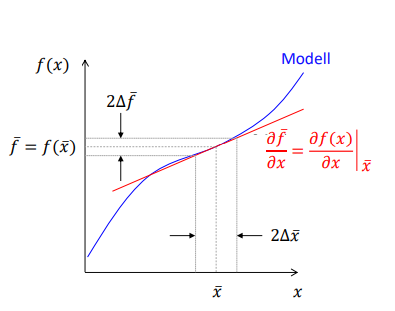
\includegraphics[width=0.5\textwidth]{Figures/gauss1D.png}
\caption{Veranschaulichung des Prinzips der Gausschen Fehlerfortplanzung im eindimensionalen Fall.}
\end{figure}

Wir betrachten nun den etwas komplizierteren Fall, in dem unsere Zielgrösse $f(x,y)$ von zwei fehlerbehafteten Messgrössen $x, y$ abhängt.Analog zum eindimensionalen Fall versuchen wir, einen Zusammenhang zwischen der Varianz der Zielgrösse und den Varianzen der Messgrössen $\sigma_x, \sigma_y$ herzustellen. Hierbei verwenden wir die Taylorentwicklung erster Ordnung für beide Variablen. Der Übersichtlichkeit halber verwenden wir $\overline{f} = f(\overline{x}, \overline{y})$, $f_n = f(x_n, y_n)$ und $\frac{\partial f}{\partial x}\bigg|_{\overline{x}, \overline{y}} = \frac{\partial \overline{f}}{\partial x}$:
\begin{align}
\begin{split}
\sigma_f^2 = \frac{1}{N-1} \sum_{n=1}^N (f_n - \overline{f})^2 = \frac{1}{N-1}\sum_{n=1}^N \left( \frac{\partial \overline{f}}{\partial x} (x - \overline{x}) + \frac{\partial \overline{f}}{\partial y} (y - \overline{y})\right)^2  \\
=  \frac{1}{N-1}\sum_{n=1}^N \left[ \left(\frac{\partial \overline{f}}{\partial x}\right)^2 (x - \overline{x})^2 + \left(\frac{\partial \overline{f}}{\partial y}\right)^2 (y - \overline{y})^2 + 2\frac{\partial \overline{f}}{\partial x}\frac{\partial \overline{f}}{\partial y}(x - \overline{x})(y - \overline{y})\right] \\
= \left(\frac{\partial \overline{f}}{\partial x}\right)^2\sigma_x^2 +  \left(\frac{\partial \overline{f}}{\partial y}\right)^2\sigma_y^2 + 2\frac{\partial \overline{f}}{\partial x}\frac{\partial \overline{f}}{\partial y}\sigma_{xy}^2
\end{split}
\label{eq:Gauss2D}
\end{align}
Wie aus Gleichung \ref{eq:Gauss2D} ersichtlich wird, hängt der Fehler der Zielgrösse im mehrdimensionalen Fall zusätzlich zu den Varianzen der einzelnen Messgrössen ($\sigma_x\sigma_y$) auch noch von der sogenannten Kovarianz $\sigma_{xy}^2$ ab, die wir im folgenden Kapitel \ref{chap:korrelation:sec:kovarianz} noch genauer betrachten wollen. Den in Gleichung \ref{eq:Gauss2D} erhaltenen Ausdruck können wir auch unter Verwendung der sogenannten Kovarianzmatrix schreiben als:
\begin{align}
\sigma_f^2 = (\partial_x, \partial_y)f \begin{pmatrix}
\sigma_x^2 & \sigma_{xy}^2 \\
\sigma_{xy}^2 & \sigma_y^2 
\end{pmatrix} \begin{pmatrix}
\partial_x \\
\partial_y 
\end{pmatrix} f
\end{align}
Dieser Formalismus kann auf beliebig viele Variablen erweitert werden, mit entsprechend höherer Dimensionalität der Kovarianzmatrix. Für unkorrelierte Variablen (d.h. alle Kovarianzen sind null, die Kovarianzmatrix ist diagonal) erhalten wir mit diesem Verfahren der Fehlerfortpflanzung:
\begin{align}
\sigma^2_f &= \sum^N_{n=1} \left( \frac{\partial f}{\partial x_n} \right)^2 \sigma^2_{x_n}\,,
\label{eq:GaussnD}
\end{align}
\begin{align}
\sigma_f &= \sqrt{ \sum^N_{n=1} \left( \frac{\partial f}{\partial x_n} \right)^2 \sigma^2_{x_n}}\,.
\label{eq:vl3-4}
\end{align}
Folglich gilt für unkorrelierte Variablen, dass die Varianz der Summe gleich der Summe der Varianzen ist.\\

Dies ist die sogenannte \textbf{Gauss-Methode} der Fehlerrechnung. Sie setzt voraus, dass:
\begin{itemize}
    \setlength\itemsep{0em}
        \item die $\sigma_n$ klein genug sind, um eine lineare Taylor-Approximation annehmen zu dürfen.
        \item die $x_n$ statistisch unabhängig sind, so dass gilt: $\text{var} ( x_1 + x_2 ) = \text{var} ( x_1 ) + \text{var} ( x_2 )$. Falls die $x_n$ nicht statistisch unabhängig sind, nennen wir sie korreliert und es treten zusätzliche Kovarianzen auf (siehe Kapitel \ref{chap:korrelation}) 
\end{itemize}

Wir wollen die Gaussche Fehlerfortpflanzung nun für unser Beispiel der Bestimmung der Erdbeschleunigung mittels der Messung der Schwingungsperiode  und Länge eines Fadenpendels verwenden. Wir messen die Schwingungsperiode \gls{gl:T_Periode}  zu:
\begin{align*}
\gls{gl:T_Periode} = \bigl( \underarrow[\text{2.50}][\uparrow]{\text{$\overline{T}$}} \pm \underarrow[\text{0.08}][\uparrow]{\text{$\sigma_T$}} \bigr) \text{s}
\end{align*}
und die Fadenlänge \gls{gl:l}  zu:
\begin{align*}
\gls{gl:l} = \bigl( \underarrow[\text{1.55}][\uparrow]{\text{$\overline{l}$}} \pm \underarrow[\text{0.02}][\uparrow]{\text{$\sigma_l$}} \bigr) \text{m}\,.
\end{align*}

Mit der Fehlerfortpflanzung nach Gauss ergeben sich folgende partielle Ableitungen:
\begin{align}
\frac{\partial \gls{gl:g}}{\partial \gls{gl:T_Periode}} = - \frac{8 \pi^2 \gls{gl:l}}{\gls{gl:T_Periode}^3},
\end{align}
\begin{align}
\frac{\partial \gls{gl:g}}{\partial \gls{gl:l}}  =   \frac{4 \pi^2}{\gls{gl:T_Periode}^2}.
\label{eq:vl3-7}
\end{align}
Damit folgt letztendlich:
\begin{align}
\sigma_g = \sqrt{ \left(  - \frac{8 \pi^2 \gls{gl:l}}{\gls{gl:T_Periode}^3} \right)^2 \sigma^2_T + \left(\frac{4 \pi^2}{\gls{gl:T_Periode}^2} \right)^2 \sigma^2_l }\,,
\label{eq:vl3-8}
\end{align}
wobei wir $\overline{T}$ und $\overline{l}$ einsetzen.



\subsection{Signifikante Stellen}
Aus den vorangegangenen Diskussionen dieses Kapitels haben Sie bereits gelernt, dass keine experimentell gemessene Zahl absolut genau ist. Dieser Umstand sollte sich auch in der Anzahl Stellen widerspiegeln, mit denen ein numerisches Resultat angegeben wird. Es ist wichtig, Resultate mit der richtigen Anzahl Stellen anzugeben, denn zu viele angegebene Stellen suggerieren eine falsche Genauigkeit. Die Anzahl Stellen vor und hinter dem Komma, die man mit Sicherheit angeben kann, wird als \textit{Anzahl signifikanter Stellen} bezeichnet. \\

%Als Daumenregel gilt: Ein Resultat sollte nicht mehr signifikante Stellen haben als der ungenaueste Wert, der zur Berechnung verwendet wurde.
Wir runden Zahlen auf die letzte Ziffer, die vom berechneten Messfehler betroffen ist. Der Messfehler wiederum wird üblicherweise auf eine signifikante Stelle gerundet. Zum Beispiel würden wir das Ergebnis der Messung einer Masse mit Mittelwert $m = 3.25118$ kg mit Standardabweichung $\sigma_m =0.02$ kg angeben als $m=3.25\text{ kg}\pm 0.02  
 \text{ kg}$. Wir haben folgende Optionen, um Standardfehler (Fehler des Mittelwerts) anzugeben:
 \begin{enumerate}
     \item[-] Absoluter Fehler $x + \Delta x$, z.B. Die Masse beträgt $m=3.25\text{ kg}\pm 0.02$ kg  
     \item[-] Relativer Fehler  $x + \frac{\Delta x}{x}$, z.B. Die Masse beträgt $m=3.25\text{ kg}\pm 1\%$ 
     \item[-] Implizite Angabe, z.B. Die Masse beträgt $m=3.25\text{ kg}$. Hier wird angenommen, dass die Zahl nicht genauer bekannt ist als die Hälfte der letzten angegebenen Ziffer (d.h. hier $\pm 0.005$).
 \end{enumerate}
%\subsection{Mit Monte-Carlo Simulationen }
%Es sei wieder die Funktion $f ( x_1, x_2, x_3, ..., x_n )$ im nachfolgenden unser Modell mit dem Beispiel der Amplitude eines Resonators: $A = f ( S, g, V_\text{in}, f, ... )$.\\[0.3cm]
%Als Monte Carlo Simulation bezeichnen wir ein ``numerisches Experiment'', in dem wir einen Wert viele Male mit zuf\"allig verteilten Anfangswerten berechnen. Die Anfangswerte können einer beliebigen PDF folgen.
%\begin{itemize}
%    \setlength\itemsep{0em}
%        \item[$-$] Keine analytische L\"osung.
%       \item[$-$] MC Simulation kann sehr rechenintensiv sein.
%        \item[$+$] Beliebig nichtlineare und komplexe Fehler berechenbar.
%        \item[$+$] Nicht auf normalverteilte \gls{gl:PDF}s beschr\"ankt.
%\end{itemize}


\newpage


\begin{tcolorbox}[enhanced,width=6in,
    fontupper=\small,drop fuzzy shadow southwest,
    colframe=black!50!black,colback=black!5]
\textbf{Verständnisfragen:} \\
\begin{enumerate}
\item[1] Wodurch entstehen Abweichungen zwischen dem
gemessenen Mittelwert und dem «Literaturwert»?
\item[2] Wodurch entsteht eine Standardabweichung in der
gemessenen Verteilung von Messwerten?
\item[3] Wie verändert sich nach wiederholtem Messen der Fehler in der
Abschätzung des Erwartungswertes ($\Delta\mu$) und die Standardabweichung ($\sigma$)?
\item[4] Kann der Fehler in der Abschätzung des Erwartungswertes $\Delta\mu$ kleiner werden als die Standardabweichung $\sigma$?
\end{enumerate}
\end{tcolorbox}

\begin{tcolorbox}[enhanced,width=6in,
    fontupper=\small,drop fuzzy shadow southwest,
    colframe=black!50!black,colback=black!5]
\textbf{Antworten:} \\
\begin{enumerate}
\item[1] Für unendlich viele Messpunkte tragen nur
systematische Fehler zu dieser Abweichung bei. Für
endlich viele Messpunkte werden auch statistische
Fehler wichtig.
\item[2] Die Standardabweichung ist ein gängiges Mass für die
statistische Streuung von Messwerten.
\item[3] $\sigma$ bleibt unverändert, aber $\Delta \mu $ wird kleiner. 
\item[4] Ja.
\end{enumerate}
\end{tcolorbox}
\chapter{Korrelierte Messgrössen}
\label{chap:korrelation}

\begin{center}
\begin{tcolorbox}[enhanced,width=6in,center upper,
    fontupper=\large,drop fuzzy shadow southwest,
    colframe=blue!50!black,colback=blue!10]
Für dieses Kapitel ist ein Jupyter-Notebook verfügbar. Siehe \gitresource{Kovarianz.ipynb} 
\end{tcolorbox}
\end{center}

Bislang haben wir in unseren Beispielen immer nur eine einzige Zufallsvariable gemessen oder Fälle betrachtet, in denen alle Zufallsvariablen voneinander unabhängig waren. In realen Experimenten treten allerdings häufig Korrelationen der Messgrössen auf. In diesem Fall geht eine Änderung in einer Variable mit einer Änderung der anderen Variable einher. Zum Beispiel könnte die Frequenz eines Resonators mit der Raumtemperatur korreliert sein. Eine derartige Korrelation muss in die Fehleranalyse einbezogen werden, wie wir in Gleichung \ref{eq:Gauss2D} sehen. \\

Bei der Analyse und Interpretation der Korrelation ist allerdings Vorsicht geboten: Korrelation wird häufig verwendet, um einen kausalen Zusammenhang aufzuzeigen. Allerdings bedeutet das Vorliegen einer Korrelation zweier Variablen $x$ und $y$ nicht automatisch, dass ein kausaler Zusammenhang zwischen ihnen besteht. Zwei Variablen $x$ und $y$ können etwa indirekt durch eine dritte Variable $z$ verbunden sein. Wenn $z$ sowohl $x$ als auch $y$ beeinflusst, können letztere eine Korrelation aufweisen, ohne dass sie direkt kausal verbunden sind. In unserem Beispiel des Resonators könnte zum Beispiel die Luftfeuchtigkeit im Raum der Grund dafür sein, dass sowohl die Temperatur als auch die Frequenz ansteigen oder abfallen.

\section{Kovarianz}
\label{chap:korrelation:sec:kovarianz}

Um einen linearen Zusammenhang zwischen zwei Variablen aufzuzeigen, verwenden wir die geschätzte Kovarianz
\begin{align}
\gls{gl:cov}(x,y) = \frac{1}{N - 1} \sum_{n = 1}^N (x_n - \overline{x})(y_n - \overline{y})\,.
\label{eq:Kovarianz}
\end{align}
In Messungen mit vielen Datenpunkten (mit $\frac{1}{N-1}\rightarrow \frac{1}{N}$) wird diese Formel häufig vereinfacht zu:
\begin{align}
\sigma_{xy}^2 = \text{cov}(x,y) = \frac{1}{N} \sum_{n = 1}^N (x_n - \overline{x})(y_n - \overline{y}).
\label{eq:Kovarianzsimple}
\end{align}
Die Kovarianz hat die Einheit $[\sigma_{xy}^2]=[x]\times[y]$. Damit hängt der Wert der Kovarianz von den gewählten Einheiten ab und hat keine universelle Bedeutung. Beispielsweise ändert sich der Zahlenwert einer Kovarianz, wenn wir Nanometer statt Meter als Längeneinheit festlegen. Um eine einheitenlose Zahl mit einer universellen Bedeutung zu erhalten, definieren wir den normalisierten Korrelationskoeffizienten:
\begin{align}
\gls{gl:rhoxy} = \frac{ \text{cov} (x,y) }{ \sigma_x \sigma_y } \quad \in [-1,1]\,.
\label{eq:Korrelationskoeffizient}
\end{align}

Hierbei bedeutet:
\begin{align}
\rho_{xy} = 
    \begin{cases}
        0,& \text{unkorrelierte Variablen}\\
        \pm 1,& \text{maximal (anti-)korrelierte Variablen für $y =  ax$.}
    \end{cases}       
\end{align}

Die Varianzen und Kovarianzen können kompakt in der sogenannten Kovarianz-Matrix zusammengefasst werden, die Sie bereits in Anschnitt \ref{chap:fehler:sec:fehlerfortpflanzung} kennengelernt haben:
\begin{align}
\begin{pmatrix}
\sigma_x^2    & \sigma_{xy}^2 & \cdots \\
\sigma_{yx}^2 & \sigma_y^2    & \cdots \\
\vdots        & \vdots        & \ddots \\
\end{pmatrix}\,.
\end{align}

Wie oben bereits erwähnt, misst die Kovarianz allerdings nur lineare Korrelationen, nichtlineare Fälle müssen anders behandelt werden. Um das zu verdeutlichen, berechnen wir die Kovarianz für die nichtlineare Funktion $y = x^2$. Hier sei $x$ eine Zufallsvariable mit einer symmetrischen Verteilungsfunktion, das heisst $-x$ ist gleich wahrscheinlich wie $x$. Für die Kovarianz erhalten wir 
\begin{align}
    \begin{split}
        \text{cov}(x,y) &= \frac{1}{N} \sum_{n = 1}^N ( x_n - \overline{x} )( y_n - \overline{y} )\\
        &= \frac{1}{N} \sum_{n = 1}^N x_n ( x_n^2 - \overline{y} )\\
        &= \frac{1}{N} \sum_{n = 1}^N x_n^3  - \frac{1}{N} \sum_{n = 1}^N x_n \overline{y} = 0 \quad \text{f\"ur } N \rightarrow{ \infty} \, ,
    \end{split}
\end{align}
was verdeutlicht, dass nichtlineare Korrelationen mit erweiterten Methoden untersucht werden müssen. \\

Wir wollen lineare Korrelationen nun am Beispiel von einfachen trigonometrischen Funktionen veranschaulichen. Hierzu generieren wir zunächst drei künstliche, quasi analoge Signale $U_1$, $U_2$ und $U_3$. Die Signale $U_1$ und $U_3$ sind Sinusfunktionen verschiedener Amplituden, aber gleicher Frequenzen. Signal $U_2$ ist eine Kosinusfunktion mit gleicher Amplitude und Frequenz wie $U_1$. Alle Signale werden mit identischem Rauschen überlagert. 


\begin{lstlisting}[language = Python]

N = 1001 # Laenge des Datenvektors
t = np.linspace(0, N-1, N) # Zeitvektor von Punkten mit Abstand 1 in Einheit von Nanosekunden (als konkretes Beispiel)

f_sig = 0.01 # Frequenz 
Amp1 = 1.2 # Amplitude 1
Amp3 = 5.2 # Amplitude 2 
sig1 = Amp1*np.sin(2*np.pi*f_sig*t) # Signal  1  
sig2 = Amp1*np.cos(2*np.pi*f_sig*t) # Signal 2
sig3 = Amp3*np.sin(2*np.pi*f_sig*t)  # Signal 3  
noise_amp = 0.2 # Amplitude des Rauschens
noise1 = np.random.normal(0,noise_amp,N) # normalverteiltes Rauschen mit Standardabweichung noise_amp
noise2 = np.random.normal(0,noise_amp,N) # normalverteiltes Rauschen mit Standardabweichung noise_amp
noise3 = np.random.normal(0,noise_amp,N) # normalverteiltes Rauschen mit Standardabweichung noise_amp
U1 = sig1 + noise1 # addiere Rauschen zu Signal 1
U2 = sig2 + noise1 # addiere Rauschen zu Signal 2
U3 = sig3 + noise1 # addiere Rauschen zu Signal 3
\end{lstlisting}

In einem ersten Schritt können wir diese Daten nun einfach visualisieren (siehe Figur \ref{fig:Us}). Diese Darstellung lässt bereits erahnen, dass $U_1$ und $U_3$ korreliert sind, doch vor allem für  $U_1$ und $U_2$ ist aus dieser Darstellung nur schwer ersichtlich, ob tatsächlich eine Korrelation vorliegt. 

\begin{figure}[H]
\centering
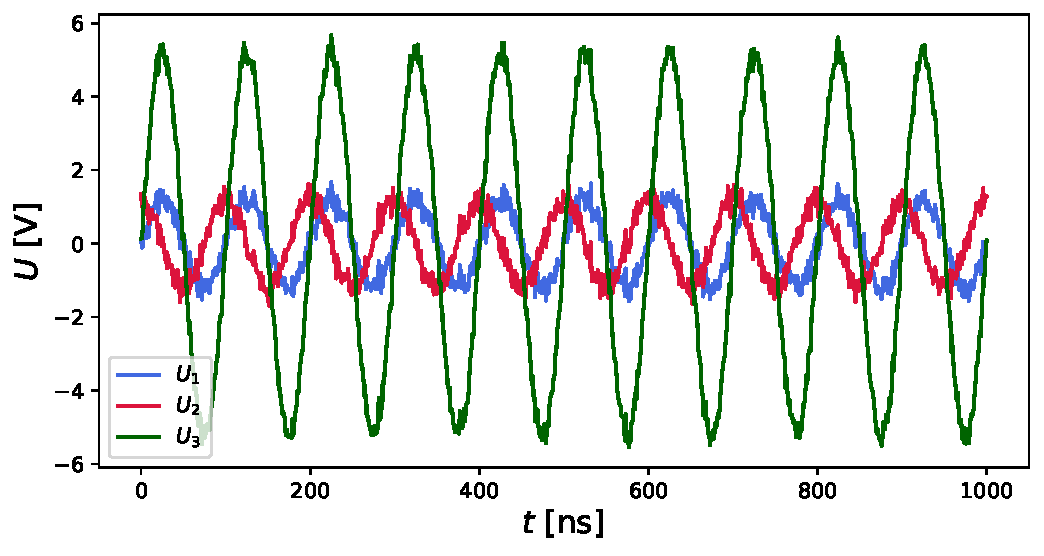
\includegraphics[width=0.75\textwidth]{Figures/Usplot.pdf}
\caption{Visualisierung der künstlich generierten, quasi-analogen und rauschbehafteten Signale $U_1$. $U_2$ und $U_3$ als Funktion der Zeit $t$.}
\label{fig:Us}
\end{figure}

Zur graphischen Überprüfung linearer Korrelation stellen wir nun $U_2$ und $U_3$ als Funktion von $U_1$ dar (siehe Figur \ref{fig:korrUs}). Aus dieser Darstellung ist direkt ersichtlich, dass $U_1$ und $U_3$ stark korreliert sind, $U_1$ und $U_2$ hingegen nur sehr schwach. Diese schwache Korrelation von $U_1$ und $U_2$ kommt dadurch zustande, dass beiden Signalen identisches Rauschen anhaftet. 

\begin{figure}[H]
\centering
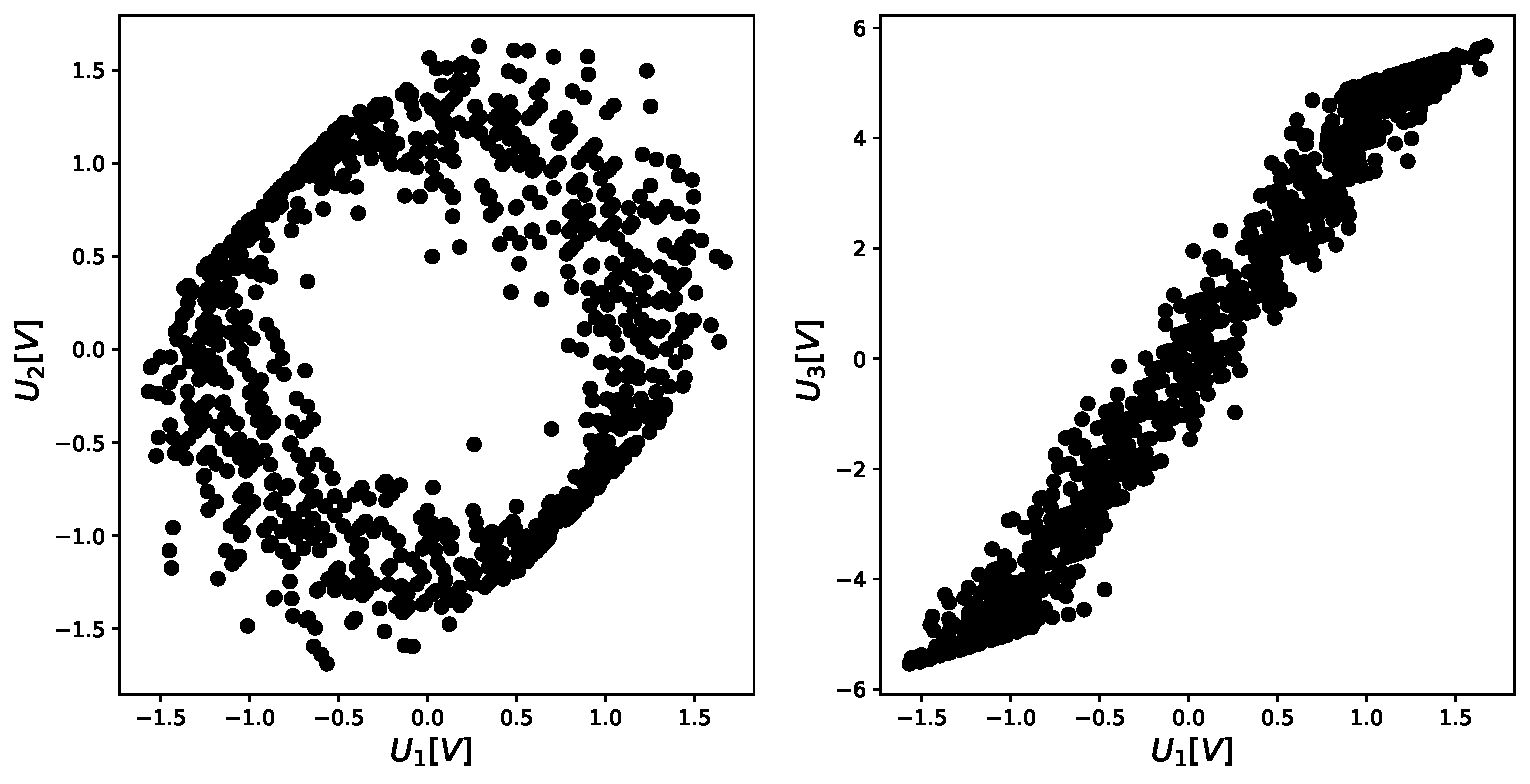
\includegraphics[width=0.75\textwidth]{Figures/Uskorrplot.pdf}
\caption{Um eine möglich Korrelation zwischen zwei Variablen graphisch zu überprüfen, stellt man die eine Variable als Funktion der anderen dar. \textbf{Links:} $U_2$ als Funktion von $U_1$. Die Punkte liegen nicht auf einer Geraden, es liegt also keine starke lineare Korrelation vor. \textbf{Rechts:} $U_3$ als Funktion von $U_1$. Wir sehen eine starke, lineare Korrelation der beiden Variablen.}
\label{fig:korrUs}
\end{figure}
Wir berechnen nun die oben eingeführte Kovarianz sowie die normalisierten Korrelationskoeffizienten.

\begin{lstlisting}[language = Python]
# U1 U3 
C = np.stack((U1,U3), axis=0)
cov13 = np.cov(C)
corcov13 = np.corrcoef(C)

# U1 U2
D = np.stack((U1, U2), axis = 0)
cov12 = np.cov(D)
corcov12 = np.corrcoef(D)
\end{lstlisting}

Die so erhaltenen Korrelationskoeffizienten $\rho_{U_1, U_2}=0.06$ und $\rho_{U_1, U_3}=0.98$ stützen unsere anfängliche, qualitative Analyse. \\

Als nächstes simulieren wir die Messung unserer quasi-analogen Signale mit einem rauschbehafteten Analog-Digital-Konvertierer (engl: Analog-Digital-Converter ADC). Das so hinzugefügte Rauschen ist nun für jedes Signal unterschiedlich. 
\begin{lstlisting}[language = Python]
Delta_t = 1 # zeitl. Abstand der Messpunkte in den gewaehlten Einheiten: fuer einen Zeitvektor t mit Abstaenden von je 1 Nanosekunde misst unser ADC einen Datenpunkt alle Delta_t Nanosekunden
U_max = 10 # maximal messbarer Wert: alle groesseren Werte werden als U_max angezeigt (clipping)
U_min = 0.01 # minimaler messbarer Spannungsunterschied der Signalwerte: Spannungsaufloesung des ADC
U_noise = 1 # Standardabweichung des Spannungsrauschens, das dem Signal durch den Messprozess hinzugefuegt wird

# Initialisierung der Messvektoren
n_mess = math.floor(N/Delta_t)-1 # Anzahl gemessener Punkte. floor rundet ab
n = range(n_mess) # wird fuer for loop benoetigt, enthaelt 0 und n_mess als untere und obere Grenze von n
t_mess = np.zeros(n_mess) # leerer Vektor, um die Zeitwerte zu erfassen
U1_mess = np.zeros(n_mess) # leerer Vektor, um die Spannungswerte zu erfassen
U2_mess = np.zeros(n_mess) # leerer Vektor, um die Spannungswerte zu erfassen
U3_mess = np.zeros(n_mess) # leerer Vektor, um die Spannungswerte zu erfassen

for i in n:
    t_mess[i] = t[(i+1)*Delta_t] # jeder (i+1)*Delta_t-te Punkt wird gemessen
    U1_mess[i] = np.clip(U_min*round((U1[(i+1)*Delta_t]+np.random.normal(0,U_noise))/U_min,0),-U_max,U_max) # numpy.clip limitiert die maximalen Werte auf [-U_max,U_max]
    U2_mess[i] = np.clip(U_min*round((U2[(i+1)*Delta_t]+np.random.normal(0,U_noise))/U_min,0),-U_max,U_max) # numpy.clip limitiert die maximalen Werte auf [-U_max,U_max]
    U3_mess[i] = np.clip(U_min*round((U3[(i+1)*Delta_t]+np.random.normal(0,U_noise))/U_min,0),-U_max,U_max) # numpy.clip limitiert die maximalen Werte auf [-U_max,U_max]
\end{lstlisting}
Wir können die so erhaltenen, ``gemessenen'' Signale $U_1^{\mathrm{mess}}$, $U_2^{\mathrm{mess}}$ und $U_3^{\mathrm{mess}}$ nun erneut als Funktionen der Zeit $t$ als auch als Funktionen von $U_1^{\mathrm{mess}}$ darstellen. 

\begin{figure}[H]
\centering
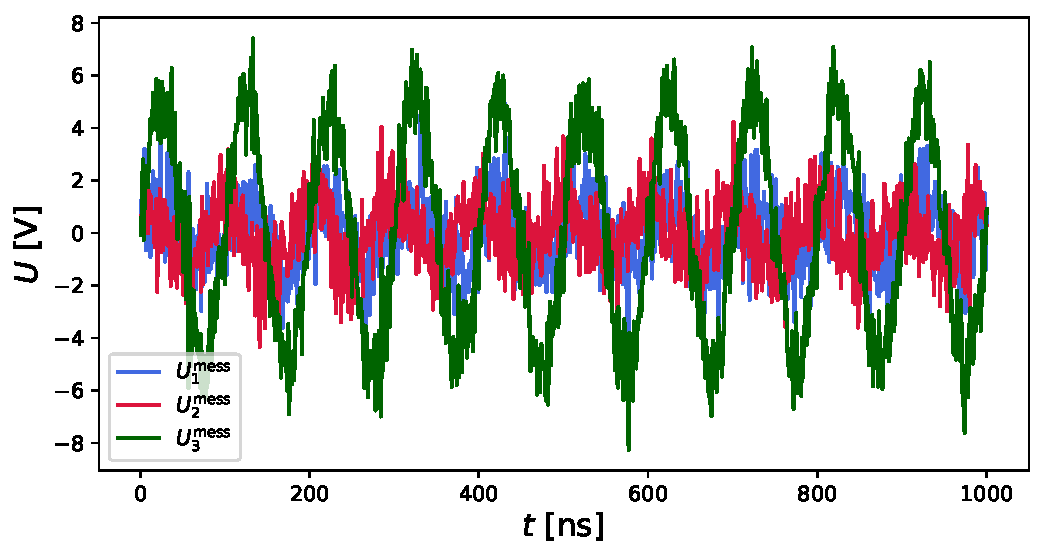
\includegraphics[width=0.75\textwidth]{Figures/Umess.pdf}
\caption{Visualisierung der künstlich generierten Signale $U_1^{\mathrm{mess}}$, $U_2^{\mathrm{mess}}$ und $U_3^{\mathrm{mess}}$ nach der Messung mit einem rauschbehafteten ADC  als Funktion der Zeit $t$.}
\label{fig:Umess}
\end{figure}

Sowohl die Darstellung in Abbildung~\ref{fig:Umesskorr} als auch die erneute Berechnung der Korrelationskoeffizienten zu $\rho_{U_1^{\mathrm{mess}}, U_2^{\mathrm{mess}}}=0.05$ und $\rho_{U_1^{\mathrm{mess}}, U_3^{\mathrm{mess}}}=0.63$ ergeben, dass das Hinzufügen dieses unkorrelierten Rauschens die Korrelation der Signale reduziert hat. Dieses einfache Beispiel verdeutlicht, dass in einem realen Messvorgang Korrelationen einzelner Variablen durch zu starkes Rauschen reduziert, bzw. vollkommen maskiert werden können.


\begin{figure}[H]
\centering
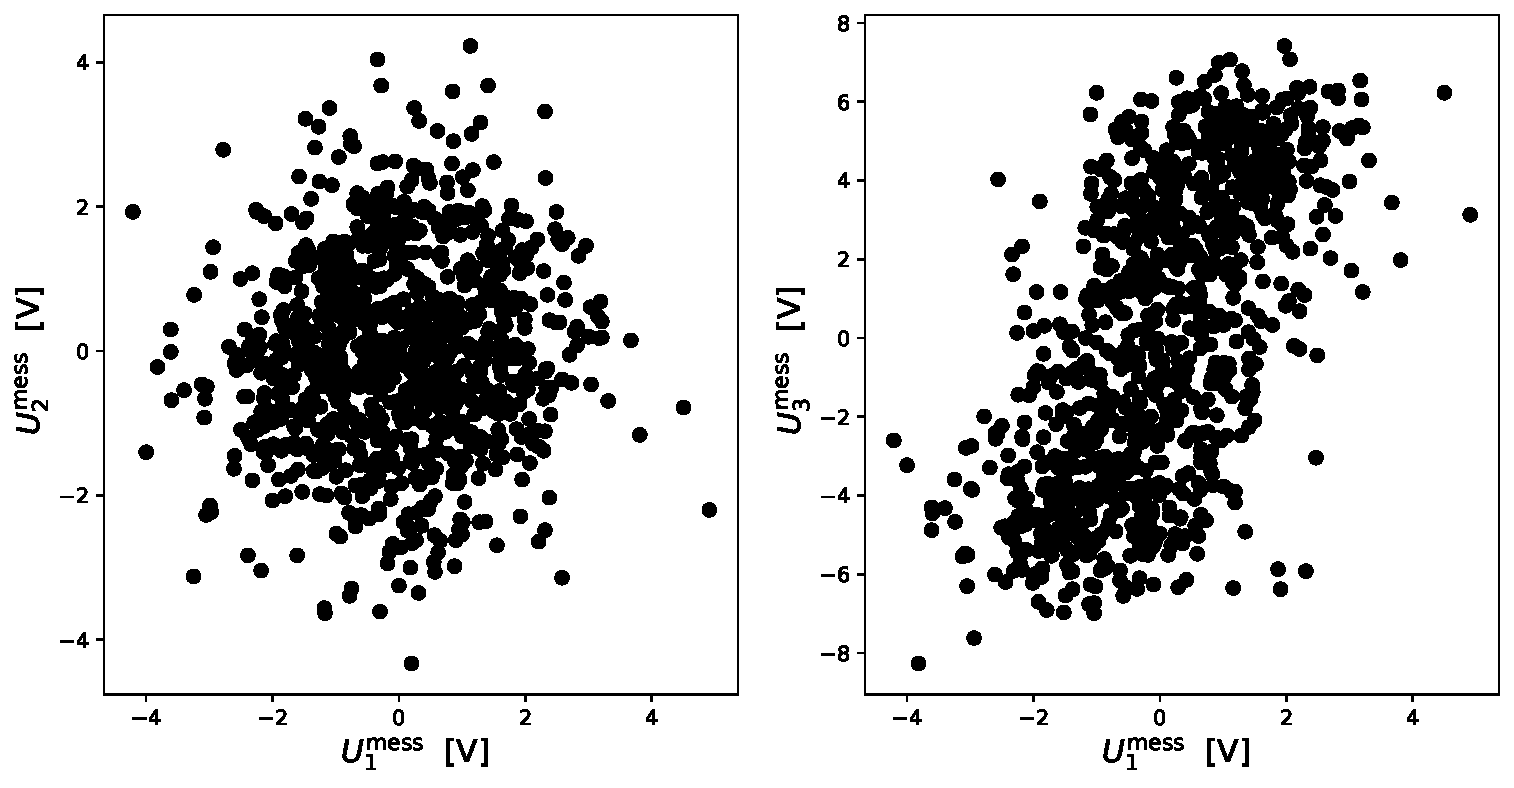
\includegraphics[width=0.75\textwidth]{Figures/Umesskorrplot.pdf}
\caption{Korrelationen zwischen den Signalen, nachdem sie von einem simulierten ADC (mit Rauschen) gemessen wurden.\textbf{Links:} $U_2^{\mathrm{mess}}$ als Funktion von $U_1^{\mathrm{mess}}$. \textbf{Rechts:} $U_3^{\mathrm{mess}}$ als Funktion von $U_1^{\mathrm{mess}}$.}
\label{fig:Umesskorr}
\end{figure}

Wir fassen zusammen: Ob zwei Signale korreliert sind oder nicht, ist nicht davon abhängig, ob sie Rauschen enthalten. Korrelation (selbst starke) kann beispielsweise durch korreliertes Rauschen entstehen. Gleichzeitig müssen rauschfreie Signale nicht korreliert sein, selbst wenn sie, wie in Abbildung~\ref{fig:Us}, dieselbe Frequenz haben.


\section{Auto-Kovarianz}
\label{chap:korrelation:sec:autokovarianz}


%Setzt man in \cref{eq:covariancesimplified} $y = x$ ein, erhält man die Varianz:
%\begin{align}
%\text{cov}(x,x) = \frac{1}{N} \sum_{n = 1}^N (x_n - \overline{x})^2 = \text{var} (x) = \sigma_x^2.
%\end{align}
Häufig sollen nicht zwei verschiedene Messgrössen miteinander korreliert werden, sondern eine Messgrösse mit sich selbst in Abhängigkeit einer Zeitverschiebung. Durch Einsetzen von $y = x_{i+\Delta}$ in Gleichung \ref{eq:Kovarianz}  erhält man die diskrete Auto-Kovarianz, also die Korrelation der Funktion $x$ mit sich selber in Abhängigkeit einer Indexverschiebung $\Delta$
\begin{align}
\gls{gl:RxxDelta} = \frac{1}{N} \sum_{n = 1}^N (x_n - \overline{x})(x_{n+\Delta} - \overline{x}). \label{eq:AutokovarianzDeskret}
\end{align}

Analog zum Korrelationskoeffizienten definieren wir den Autokorrelationskoeffizienten
\begin{align}
\gls{gl:rhoxx} = \frac{ R_{xx} (\Delta) }{ \sigma_x^2 } \quad \in [-1,1]\,.
\end{align}
In vielen Anwendungen sind wir an der diskreten Autokovarianz als Funktion der Zeitverschiebung $\tau = \Delta \times \delta t$ interessiert und verwenden diese Zeitverschiebung anstelle der Indexverschiebung als Variable, sodass wir 
\begin{align}
R_{xx} (\tau) = \frac{1}{N} \sum_{t = t_1}^{t_N} (x(t) - \overline{x})(x(t + \tau) - \overline{x})
\end{align}
mit dem entsprechenden Autokorrelationskoeffizienten:
\begin{align}
\rho_{xx} = \frac{ R_{xx} (\tau) }{ \sigma_x^2 } \quad \in [-1,1]\,.
\end{align}
erhalten. \\

Theoretisch existiert für kontinuierliche Funktionen auch die kontinuierliche Auto-Kovarianz
\begin{align}
\gls{gl:Rxxtau} = \lim_{T \rightarrow \infty} \frac{1}{T} \int_0^T x(t) x(t + \tau) dt = \langle x(t) x(t + \tau) \rangle \,.
\end{align}
Diese kann allerdings nicht für diskrete Signale verwendet werden und ist daher in realen Anwendungen nicht von Relevanz. Wichtige Eigenschaften der Auto-Kovarianz sind wie folgt:
\begin{itemize}
    \setlength\itemsep{0em}
        \item Die Auto-Kovarianz ist symmetrisch um $\Delta = 0$ (bzw. $\tau = 0$).
        \item Die Samplingzeit \gls{gl:deltat} (zeitlicher Abstand zwischen aufeinanderfolgenden Messpunkten) setzt ein unteres Limit für die zeitliche Auflösung der Messung, und damit für die `periodische Zeit' $\tau$.
        \item Die Auto-Kovarianz bei $\Delta = 0$ ($\tau = 0$) entspricht der Varianz und ist das Maximum der Funktion.
        \item Die Auto-Kovarianz von Gauss-verteiltem weissen Rauschen ist Null f\"ur alle $\tau \neq 0$, da weisses Rauschen per Definition von Punkt zu Punkt vollkommen unkorreliert ist.
        \item Die Auto-Kovarianz einer perfekten Sinuswelle ist als Funktion von $\tau$ perfekt periodisch, da Punkte über jede Periode (und damit über jedes ganzzahlige Mehrfache der Periode) perfekt korreliert sind.
\end{itemize}

Die Auto-Kovarianz ist geeignet, um periodische zeitliche Zusammenhänge zu sehen. Ein typisches Beispiel ist die Bestimmung der Korrelationszeit (``Kohärenzzeit'') aus der Breite des Maximums um $\tau = 0$. Aperiodische zeitliche Information (wie z.B. ein kurzer Signalpuls) ist darin aber nicht mehr sichtbar.

Wir wollen nun für unser im Kovarianz-Kapitel eingeführtes Test-Signal $U_1$ die Auto-Kovarianz berechnen. Hierfür definieren wir zunächst die entsprechende Auto-Kovarianzfunktion und wenden diese auf $U_1$ an.
\begin{lstlisting}[language = Python]
# definiere Auto-Kovarianzfunktion
def Rxx(x, delta):
    xm = np.mean(x)
    dev_sum = 0
    for i in range(len(x) - delta):
        dev_sum += (x[i] - xm) * (x[i + delta] - xm)
    return dev_sum / (len(x) - delta)

# wende Funktion auf Beispiele an 
delta_max = len(U1)
Rxx_vs_delta = [Rxx(U1, i) for i in range(delta_max)]
lags = np.linspace(0, delta_max, num=delta_max)
\end{lstlisting}
Da $U_1$ eine Sinusfunktion ist,  erreicht die Auto-Kovarianzfunktion in periodischen Abständen Maxima und Minima (siehe   \ref{fig:AutokorrelationU1}). Wenn $\Delta$ dem Vielfachen einer Periode von $U_1$ entspricht, liegt eine hohe Korrelation vor, nach ungeraden Vielfachen einer halben Periode von $U_1$ eine hohe Anti-Korrelation.   
\begin{figure}[H]
\centering
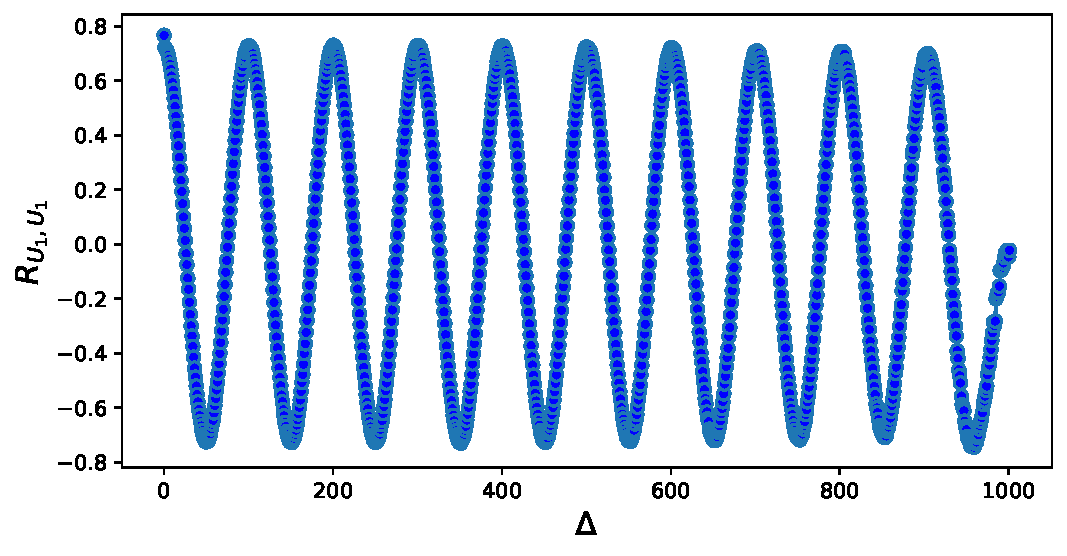
\includegraphics[width=0.75\textwidth]{Figures/U1Auto.pdf}
\caption{Autokorrelationsfunktion $R_{U_1U_1}(\Delta)$ von $U_1$ als Funktion der Indexverschiebung $\Delta$.}
\label{fig:AutokorrelationU1}
\end{figure}




\begin{center}
\begin{tcolorbox}[enhanced,width=6in,drop fuzzy shadow southwest,
colframe=blue!50!black,colback=blue!01]
\textbf{Anwendungsbeispiel}: Ultraschnelle Laserphysik \\
Ein reales Anwendungsgebiet der  Autokorrelation ist die  ultraschnelle Laserphysik (Engl: Ultrafast Laser Physics). Die Charakterisierung von ultraschnellen optischen Pulsen gestaltet sich häufig  schwierig, weil die verfügbaren elektrischen Techniken nur über eine limitierte Zeitauflösung (1-10 Picosekunden) verfügen, die Dauer der Pulse allerdings nur wenige Femtosekunden beträgt. Um solche kurzen Pulse dennoch zu messen, wird das Verfahren der sogenannten \textit{Optical Intensity Autocorrelation} angewandt. Der Laserstrahl wird zunächst in zwei Laserstrahlen gleicher Intensität geteilt. Einer der beiden Strahlen wird gegenüber dem anderen Strahl um eine Zeit $\tau$ verzögert, indem die Länge des optischen Pfades dieses Strahles entsprechend angepasst wird. Anschliessend werden die beiden Strahlen mithilfe eines nichtlinearen Kristalls  wieder überlagert und detektiert. Die Intensität des gemessenen Signales ist abhängig von der Verzögerung $\tau$ und entspricht aus mathematischer Sicht einer Autokorrelationsfunktion. Mit diesem experimentellen Aufbau kann mit höherer Zeitauflösung das Intensitätsprofil des Eingangsstrahls bestimmt werden. 
\end{tcolorbox}
\end{center}



\begin{tcolorbox}[enhanced,width=6in,
    fontupper=\small,drop fuzzy shadow southwest,
    colframe=black!50!black,colback=black!5]
\textbf{Verständnisfragen:} \\
\begin{enumerate}
\item[1] Welche Funktion ist nützlich, um einen systematischen
Zusammenhang zwischen zwei Variablen aufzuzeigen?
\item[2] In einem Experiment tauchen zwei Quellen von statistischen
Fehlern auf ($\sigma_x$ und $\sigma_y$). Unter welchen Bedingungen kann
der gemessene Fehler $\sigma_f$ kleiner sein als die beiden
einzelnen Fehlerquellen?
\end{enumerate}
\end{tcolorbox}

\begin{tcolorbox}[enhanced,width=6in,
    fontupper=\small,drop fuzzy shadow southwest,
    colframe=black!50!black,colback=black!5]
\textbf{Antworten:} \\
\begin{enumerate}
\item[1] $\frac{1}{N} \sum_{n = 1}^N (x_n - \overline{x})(y_n - \overline{y})$
\item[2] Wenn die beiden Messgrössen korreliert sind.
\end{enumerate}
\end{tcolorbox}
\chapter{Die Spektrale Leistungsdichte und Rauschen} \label{ch:spectral}
\begin{center}
\begin{tcolorbox}[enhanced,width=6in,center upper,
    fontupper=\large,drop fuzzy shadow southwest,
    colframe=blue!50!black,colback=blue!10]
Zur Fouriertransformation und Spektralen Leistungsdichte ist ein Jupyter-Notebook verfügbar. Siehe \gitresource{Fouriersynthese.ipynb} 
\end{tcolorbox}
\end{center}

\section{Information im Frequenzraum}\label{sec:Fourier}
\subsection{Komplexe Zahlen und Oszillationen}
\label{subsec:vl7a}
\begin{figure}[tbp]
    \centering
        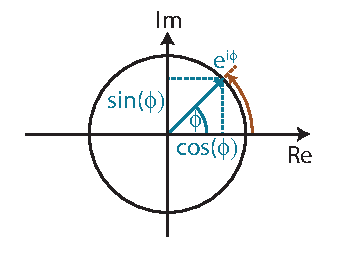
\includegraphics[width=0.4\textwidth]{Figures/complex_numbers.pdf}
        \caption{Komplexe Zahl $e^{i\phi}$ dargestellt als Vektor in der komplexen Zahlenebene. Wir können diese Zahl in Real- und Imaginärteil zerlegen, $e^{i\phi} = \cos{(\phi)} + i \sin{(\phi)}$. Wenn die Phase $\phi$ linear zeitabhängig ist, rotiert der Zahlenvektor gegen den Uhrzeigersinn.  }
        \label{fig:complexNumbers}
\end{figure}

Im Folgenden benötigen wir Exponentialfunktionen mit komplexen Argumenten, um Oszillationen darzustellen. Wir erinnern uns an die folgenden Reihenentwicklungen:
\begin{align}
&e^{\phi} = 1 + \phi + \frac{\phi^2}{2!} + \frac{\phi^3}{3!} + ... \nonumber\\
&\cos{\phi} = 1 - \frac{\phi^2}{2!} + \frac{\phi^4}{4!} - ...\nonumber\\
&\sin{\phi} = \phi - \frac{\phi^3}{3!} + \frac{\phi^5}{5!} - ...\,.
\label{eq:vl7a-1}
\end{align}
Hier nennen wir $\phi$ eine ``Phase''. Durch Einsetzen können wir überprüfen, dass ausserdem gilt
\begin{align}
&e^{i\phi} = \cos{\phi} +i\sin{\phi}\,.
\label{eq:vl7a-2}
\end{align}
Wenn die Phase linear von der Zeit abhängig ist, setzen wir $\phi = \omega t$ ein und erhalten eine Rotation in Gegenuhrzeigersinn in der komplexen Ebene:
\begin{align}
&e^{i\omega t} = \cos{\omega t} +i\sin{\omega t}\,.
\label{eq:vl7a-3}
\end{align}
Generell führen zeitabhängige reelle Argumente in der Exponentialfunktion entweder zu einem Wachstum oder einer Abnahme, je nach Vorzeichen. Imaginäre Argumente dagegen führen zu einer Oszillation. Die Form in \cref{eq:vl7a-3} ist sehr praktisch, um harmonische Oszillationen darzustellen, da man den Realteil der Funktion mit der Auslenkung $x(t)$ identifizieren kann und den Imaginärteil mit der entsprechenden zeitlichen Ableitung $\dot{x}/\omega$ (die Teilung durch $\omega$ ist nötig, um dieselbe Einheit wie für $x$ zu erhalten). Damit das Vorzeichen der Ableitung stimmt, benutzen wir für die Darstellung harmonischer Oszillatoren oft
\begin{align}
&e^{-i\omega t} = \cos{\omega t} -i\sin{\omega t}\,.
\label{eq:vl7a-4}
\end{align}
Das negative Vorzeichen entspricht einer Rotation in der komplexen Ebene im Uhrzeigersinn.

\subsection{Die Diskrete Fouriertransformation (DFT)}
\label{subsec:vl7}

Sei $x(t)$ eine Timetrace (d.h. gemessene Werte als Funktion der Zeit). 
Können wir die verschiedenen Frequenz-Komponenten dieses Signals einfach darstellen?  
Dafür ist folgendes Theorem wichtig: 
% und $R_{xx} (\tau)$ die zugehörige Auto-Kovarianz aus \cref{eq:AutokovarianzDeskret}, welche Information über die periodischen Signale in $x(t)$ wiedergibt. Gibt es eine Möglichkeit, die in $R_{xx} (\tau)$ enthaltenen Frequenzen einfach auszulesen?

\begin{center}
\begin{tcolorbox}[enhanced,width=6in,drop fuzzy shadow southwest,
    colframe=red!50!black,colback=red!05]
   Fouriers Theorem: Jede integrierbare Funktion kann als Summe von trigonometrischen Funktionen dargestellt werden.
\end{tcolorbox}
\end{center}


Diese Theorem führt zur \textbf{Fouriertransformation}. In dieser Vorlesung beschäftigen wir uns insbesondere mit der diskreten Fouriertransformation (DFT), da alle gemessen Signale sowohl in der Zeit als auch in der Auslenkung diskret sind (d.h., nur gewisse Werte annehmen). 
Mit der Exponentialschreibweise nimmt die DFT eines Signals $x(t)$ de folgende Form an: 

\begin{equation}
    x(t_k)= \sum_{n=-N/2}^{N/2} X(f_n) e^{i 2 \pi f_n t_k} 
\label{eq:vl7-1a}
\end{equation}

wobei $\Delta_f=1/t_\mr{tot}$ die kleinste Frequenzdifferenz ist, die in der Messzeit $t_\mr{tot}$ aufgelöst werden kann, und $f_n = n \Delta_f$ ist die $n$-te diskrete Frequenz, die wir als Funktion der diskreten Zeit $t_k = k\Delta_t$ betrachten. \\
Die komplexen Koeffizienten $X(f)$ geben an, wie gross die Amplitude der DFT an einer bestimmten Frequenz ist. Diese Koeffizienten können mit einer Rücktransformation bestimmt werden: 
\begin{equation}
    X(f_n)= \frac{1}{N}\sum_{k=0}^{N-1} x(t_k) e^{-i 2 \pi f_n t_k} 
\label{eq:vl7-1b}
\end{equation}
Wir können die $X(f_n)$ als Kovarianz zwischen dem Signal $x(t)$ und einem Testsignal $e^{-i 2 \pi f_n t_k}$ an der Frequenz $f_n$ vorstellen. $X(f_n)$ gibt also an, wie gut die beiden Signale übereinstimmen. Ob die Normierung $1/N$ in der Hin- oder in der Rücktransformation erfolgt, ist frei wählbar (es müssen aber andere Formeln entsprechend angepasst werden, siehe unten).
Abb. \ref{fig:fouriertransformation} zeigt ein Beispiel für eine Fouriertransformation.   \\

\begin{figure}[htbp]
    \centering
        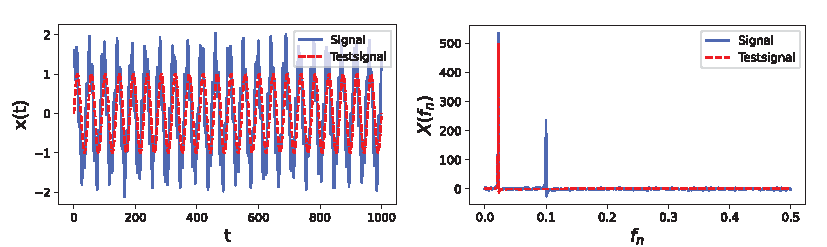
\includegraphics[width=\textwidth]{Figures/psd_fig1.pdf}
        \caption{Beispiel Fouriertransformation: Das gemessen Signal enthält zwei dominante Frequenzkomponenten, von denen eine mit dem Testsignal übereinstimmt. \textbf{Links:} Signal $x(t)$ and Testsignal $e^{i2\pi f_n t_k}$ \textbf{Rechts:} Fouriertransformation von $x(t_k)$ und vom Testsignal.}
        \label{fig:fouriertransformation}
\end{figure}
% Sei $F(x)$ eine integrierbare kontinuierliche Funktion. Dann ist $\tilde{F}(\xi)$ deren Fouriertransformierte (und umgekehrt). Es gilt:
% \begin{align}
% \tilde{F}(\xi)= \int_{-\infty}^{\infty} F(x) e^{-i 2 \pi \xi x}dx \nonumber\\
% {F}(x)= \frac{1}{2\pi}\int_{-\infty}^{\infty} \tilde{F}(\xi) e^{i 2 \pi \xi x}d\xi\,.
% \label{eq:vl7-1a}
% \end{align}
% Im Fall von diskreten Signalen definieren wir analog die diskrete Fouriertransformation (DFT) für die Funktion $F(x)$:
% \begin{align}
% \tilde{F}(\xi)= \sum_{n=0}^{N} F(x) e^{-i 2 \pi \xi x} \Delta x \nonumber\\
% {F}(x)= \frac{1}{2\pi}\sum_{n=0}^{N} \tilde{F}(\xi) e^{i 2 \pi \xi x}\Delta\xi\,,
% \label{eq:vl7-1b}
% \end{align}
% wobei $\Delta x$ (bzw. $\Delta \xi$) die Schrittgrösse in der jeweiligen Variable ist. 
Man beachte, dass die rein mathematische Definition der DFT für eine einheitenlose Zahlenfolge $x_n$ einfacher aussieht:
\begin{align}
X_k = \sum_{n=0}^{N-1} x_n e^{-i 2 \pi k n/N}\,.
\label{eq:vl7-1c}
\end{align}
Hier sind sowohl $x_n$ als auch die transformierte Zahlenfolge $X_k$ Zahlen ohne physikalische Bedeutung. Die Schrittgrösse, welche die Rolle einer diskreten Integrationsvariablen einnimmnt, reduziert sich hier auf $1$ und wird unsichtbar. Diese Formel kann also nicht direkt auf physikalische Signale mit Einheiten angewendet werden. In Python, MATLAB oder anderen Programmen, wo die Fouriertransformation mit Hilfe der ``fast Fourier transform'' FFT (einer effizienten Variante der DFT) berechnet wird, muss man daher das Resultat der FFT nachträglich mit der Schrittgrösse normieren. Generell ist immer Vorsicht geboten, wenn man einen Software-Algorithmus zum ersten Mal verwendet, da die Normierung nicht immer gleich implementiert ist. Im numpy-Paket von Python entspricht beispielsweise die funktion numpy.fft in unserer Notation nicht $X(f_n)$, sondern $NX(f_n)$. Man berechnet dann den spektralen Koeffizienten $X(f_n)$ einer Messreihe $x(t)$ mit dem folgenden Code: 
\begin{lstlisting}[language = Python]
FFTx = np.fft.fft(x)/N # fast Fourier transform von x(t) mit N Messwerten
Xn = FFTx[n] # Fourierkoeffizient mit Index n (fuer Details siehe Dokumentation)
\end{lstlisting}

Die Fouriertransformation kann entweder nur für positive (einseitig, single-sided) oder für positive und negative Frequenzen (zweiseitig, double-sided) definiert werden. In der zweiseitigen DFT eines Signals mit $N$ Punkten in der Zeit liegen im Frequenzraum ebenfalls $N$ Punkte vor, die zwischen den maximalen Frequenzen $\pm f_{max}$ (siehe unten) verteilt sind. Negative Frequenzen haben keine zusätzliche Bedeutung; die Fouriertransformation ist symmetrisch im Realteil (bzw. antisymmetrisch im Imaginärteil). Aus diesem Grund werden die negativen Frequenzanteile oft weggelassen und man erhält $N/2$ Punkte zwischen null und $f_{max}$.

\subsection{Eigenschaften der DFT}
\begin{itemize}
\item \textbf{Maximale Frequenz}: Die maximale Frequenz, die ohne Aliasing gesampelt werden kann, ist die sogenannte Nyquist-Frequenz:
        \begin{align}
        f_{max} = \frac{ 1 }{ 2 \Delta_t }\,.
        \label{eq:vl7-4}
        \end{align}
        Signale höherer Frequenz können mit derselben Samplingrate nicht richtig interpretiert werden und erzeugen im Spektrum Spitzen bei falschen Frequenzwerten.
        \begin{center}
        \begin{tcolorbox}[enhanced,width=6in,drop fuzzy shadow southwest,
            colframe=red!50!black,colback=red!05]
           Diese Limite für korrekt gemessene Frequenzen nennt man das Nyquist-Kriterium.
        \end{tcolorbox}
        \end{center}
        \item \textbf{Frequenzaufl\"osung}: Frequenzen können unterschieden werden, wenn über die gesamte Messzeit $t_\mr{tot}=N\Delta t$ mindestens eine volle Oszillation Unterschied entsteht, also $\Delta_t \leq 1/t_\mr{tot}$. Damit erhalten wir die Aufl\"osung:
        \begin{align}
        \delta f  = \frac{ 1 }{t_{tot}} = \frac{ 1 }{ N \Delta_t} = \frac{ 2 f_{max} }{ N }
        \label{eq:vl7-6}
        \end{align}
        mit $N$ Punkten von $-f_{max}$ bis $+f_{max}$. Die Frequenzwerte, an denen die DFT ausgwertet wird, entsprechen einer ganzen Zahl $n$ mal der Aufl\"osung:
        \begin{align}
        f_n = n \times \Delta_f\,.
        \label{eq:vl7-7}
        \end{align}
        \item Die PSD einer perfekten, unendlich lange gemessenen Sinuswelle hat einen einzelnen Peak bei der Wellenfrequenz und ist überall sonst gleich null. Perfektes weisses Rauschen hat über das gesamte Spektrum denselben Wert.
\end{itemize}

% Die Fouriertransformierte ist generell komplexwertig, wobei die Phase der komplexen Zahl $X(f_k)$ (bei einem bestimmten Wert von $\xi$) der Phase des Signals entspricht. Der reelle Teil von $\tilde{F}(\xi)$ gibt also den Cosinus-Anteil an, der imaginäre Teil den Sinus-Anteil. \\

% Angewendet auf unsere experimentelle Zahlenfolge $x(t)$, sieht das so aus: 
% \begin{equation}
%     x(t) = \sum_{n=-\infty}^{\infty} c_n e^{in2\pi\Delta_f t}~,
% \end{equation}
% wobei $\Delta_f=\frac{1}{t_{tot}}$ die kleinste Frequenz(differenz) ist, die in der Messzeit $t_{tot}$ aufgelöst werden kann. 
% Die komplexen Koeffizienten $c_n$ können mit einer Fouriertransformation bestimmt werden: 
% \begin{align}
%     c_n(f) & = \frac{1}{t_{tot}} \int_{t=0}^{t_{tot}} x(t) e^{-i2\pi f t} dt & \mathrm{Kontinuierliche~Fouriertransformation} \\
%     c_n(f) & =  \frac{1}{t_{tot}} \sum_{n=0}^N x(n\Delta_t) e^{-i2\pi f n \Delta_f} \Delta_t & \mathrm{Diskrete~Fouriertransformation} 
% \end{align}

\section{Die Spektrale Leistungsdichte}\label{sec:WienerKhinchin}

%\subsection{Die Spektrale Leistungsdichte -- Power Spectral Density (PSD)}
%\label{subsec:vl7-2}

In vielen Anwendungen sind wir nicht an der Phase oder dem Vorzeichen einer Fourierkomponente interessiert, sonder nur daran, wieviel Leistung in einem bestimmten Frequenzintervall enthalten ist. Beispielsweise kann es wichtig sein, wiviel Leistung eine Lichtquelle im sichtbaren Teil des elektromagnetischen Spektrums abstrahlt. In derartigen Fällen wird das normierte Quadrat der Fouriertransformation verwendet – die sogenannte Leistungsdichte oder power spectral density (PSD):
\begin{align}
S_{xx} (f) = \frac{\Delta_t}{N} \left| \sum_{k=0}^{N-1} x(t_k) e^{-i 2 \pi f_n t_k} \right|^2 = \Delta_t
N \left| X(f_n) \right|^2 \,,
\label{eq:vl7-3}
\end{align}
Mit Python lässt sich die gesamte PSD aller Frequenzen beispielsweise so berechnen:
\begin{lstlisting}[language = Python]
FFTx = np.fft.fft(x)/N # normierte FFT von x(t), d.h. Liste von Fourierkoeffizienten von x(t) mit N Messwerten
PSD = dt*N*np.abs(FFTx)**2
\end{lstlisting}


% \begin{figure}[htbp]
%     \centering
%     \begin{subfigure}[b]{0.49\textwidth}
%         \includegraphics[width=\textwidth]{Figures/psd-fig2.pdf}
%         \caption{Signal $x(t)$ mit gemessenen Punkten angenommen wir messen einmal pro s }
%         \label{fig:PSD_sub1}
%     \end{subfigure}
%     \hfill
%     \begin{subfigure}[b]{0.49\textwidth}
%         \includegraphics[width=\textwidth]{Figures/psd-fig3.pdf}
%         \caption{PSD der gemessenen Punkte (siehe .ipynb zu dieser Sektion)}
%         \label{fig:PSD_sub2}
%     \end{subfigure}
%     \caption{Beispiel PSD}
%     \label{fig:PSD}
% \end{figure}

\begin{figure}[htbp]
    \centering
        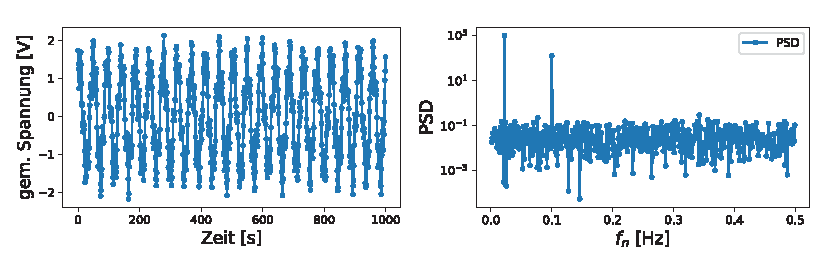
\includegraphics[width=\textwidth]{Figures/psd_fig2.pdf}
        \caption{Beispiel PSD. \textbf{Links:} Signal $x(t)$ mit gemessenen Punkten angenommen wir messen einmal pro s  \textbf{Rechts:} PSD der gemessenen Punkte (siehe .ipynb zu dieser Sektion)}
        \label{fig:PSD}
\end{figure}

Die PSD kann auch anders berechnet werden: Wenn wir die Fouriertransformation der Auto-Kovarianz $R_{xx}(t)$ aus Gl. (\ref{eq:AutokovarianzDeskret}) bilden, erhalten wir die spektrale Leistungsdichte (power spectral density, \gls{gl:PSD}) \gls{gl:S_xx}:

\begin{align}
S_{xx} (f) = \sum_{n=0}^{N} R_{xx} (\tau_n) e^{-i 2 \pi f \tau_n}\Delta \tau
\label{eq:vl7-1}
\end{align}
mit der entsprechenden Rücktransformation
\begin{align}
R_{xx} (\tau) = \frac{1}{2 \pi} \sum_{n=0}^{N} S_{xx} (f_n) e^{i 2 \pi f_n \tau}\Delta f\,.
\label{eq:vl7-2}
\end{align}

\begin{center}
\begin{tcolorbox}[enhanced,width=6in,drop fuzzy shadow southwest,
    colframe=red!50!black,colback=red!05]
   Dieser Zusammenhang zwischen der Auto-Kovarianz und der spektralen Leistungsdichte ist bekannt als das Wiener-Khinchin Theorem.
\end{tcolorbox}
\end{center}

 

Abb. \ref{fig:PSD} zeigt, wie wir das Signal $x(t)$ aus dem vorherigen Kapitel mit einem Analog-Digital-Konverter messen und dann die PSD dieser Messung berechnen. \\ 

Die Normierung mit $\Delta_t$ in Gl. (\ref{eq:vl7-3}), bzw. $\Delta_\tau$ in Gl. (\ref{eq:vl7-1}) macht aus einem Power Spectrum (mit derselben Einheit wie $x^2$) eine PSD mit der Einheit $x^2/$Hz (zum Beispiel $m^2/$Hz, $V^2/$Hz, ...). 
%\textit{Beispiel: Die PSD einer perfekten Sinuswelle hat einen Peak bei der Signalfrequenz und ist sonst \"uberall Null.}

%\begin{center}
%\textcolor{red}{Wir betrachten die Leistung (Power), also das Quadrat der diskreten Fourier-Transformation (\gls{gl:DFT}), da die Power unabh\"angig vom Vorzeichen und damit einfacher auszulesen ist.}
%\end{center}

%Weiterhin betrachten wir die spektrale Dichte anstatt dem Powerspektrum (\gls{gl:PS}, mit derselben Einheit wie $x^2$), da der PSD-Wert ($S_{xx}$) unabhängig von der Messzeit und oft relevanter als das Powerspektrum ist. Die Normierung mit $\delta t$ macht aus einem Powerspektrum eine PSD mit der Einheit $V^2$/Hz, $m^2$/Hz, $I^2$/Hz. Der gemessene Wert der PSD hängt nicht von der Frequenzauflösung ab (im Gegensatz zur PS). Eine lange und eine kurze Messung sollen dasselbe Resultat produzieren!


\subsection{Eigenschaften der spektralen Leistungsdichte (PSD)}
\label{subsec:vl7-3}

%Ist der Zeitintervall zwischen Messpunkten $\delta t \ll 1/f_{signal}$, so wird die Signalfrequenz korrekt gemessen. Ist aber der Zeitintervall zwischen Messpunkten $\delta t > 1/f_{signal}$, kann die Signalfrequenz nicht korrekt gemessen werden und diesem Fall kommt es zum ``Aliasing''.
\begin{itemize}
    \setlength\itemsep{0em}
        \item Die PSD bildet das Spektrum der Leistung, welche im Gegensatz zur Amplitude der Welle nicht von der Wellenphase abhängt. Die PSD ist also überall positiv.
        \item Die Normierung der PSD ist so gewählt, dass ihre numerische Integration über alle Frequenzen der Varianz $\sigma_x^2$ entspricht (siehe ``Parseval-Theorem'' in Sektion~\ref{subsec:vl7-4}). Deshalb muss die PSD Einheiten von $x^2/Hz$ haben. Im Gegensatz zum Leistungsspektrum, welches auch oft verwendet wird, ist der Wert der PSD an einer bestimmten Frequenz unabhängig von der Messzeit (abgesehen von statistischen Fehlern).
        \item Die PSD ist generell für positive und negative Werte von $f$ bestimmt und symmetrisch um $f=0$. Oft wird nur der positive Teil der PSD gezeigt. Dann muss die PSD mit einem Faktor 2 multipliziert werden, um die Normierung zu erhalten. Es wird deshalb immer angegeben, ob man die ``single-sided'' oder ``double-sided PSD'' benutzt.
\end{itemize}

\section{Rauschen und Parsevals Theorem}\label{sec:Parseval}
\begin{center}
\begin{tcolorbox}[enhanced,width=6in,center upper,
    fontupper=\large,drop fuzzy shadow southwest,
    colframe=blue!50!black,colback=blue!10]
    {Zu Rauschen und Parseval-Theorem ist ein Jupyter-Notebook verfügbar. Siehe \gitresource{Parseval theorem and filtering.ipynb} }
\end{tcolorbox}
\end{center}
\subsection{Parseval-Theorem}
\label{subsec:vl7-4}

Die wichtige Normierungseigenschaft der PSD, welche einen Zusammenhang zwischen der Varianz einer Variable $x(t)$ und dessen PSD herstellt, ist bekannt als das Parseval-Theorem. F\"ur 
den kontinuierlichen, doppelseitig definierten Fall lautet das Parseval-Theorem:
\begin{align}
\sigma_x^2 = \int_{- \infty}^\infty S_{xx} (f) df\,,
\label{eq:vl7-8}
\end{align}
F\"ur den diskreten, doppelseitig definierten Fall entspricht dies:
\begin{align}
\sigma_x^2 = \Delta_f \sum_{f = -f_{max}}^{f_{max}} S_{xx} (f)\,.
\label{eq:vl7-9}
\end{align}
Wenn einseitig definierte PSDs verwendet werden, muss ihr Wert mit einem Faktor 2 multipliziert werden, damit das Integral (bzw. die Summe) von null bis $f_{max}$ immer noch der Varianz entspricht.

Die PSDs unkorrelierter Variablen sind additiv, also gilt für ein Signal $x(t) = a(t) + b(t)$
\begin{equation}
        S_{xx}(f_n) = S_{aa}(f_n) + s_{bb}(f_n) \,.\label{eq:additive_PSDs}
\end{equation}
Aus dem Parseval-Thereom und Gl. (\ref{eq:additive_PSDs}) folgt dann die bereits bekannte Tatsache, dass auch die Varianzen unkorrelierter Variablen additiv sind, also 
\begin{equation}
    \sigma_x^2 = \sigma_a^2 + \sigma_b^2\,.
\end{equation}
Diese Eigenschaft können wir uns zunutze machen, um zum Beispiel ein bekanntes Detektorrauschen von einem unbekannten Signal abzuziehen, wie in der Vorlesung gezeigt. 

\subsection{Rauschen in der PSD}
\label{subsec:vl10}

% \begin{figure}[htbp]
%     \centering
%     \begin{subfigure}[b]{0.49\textwidth}
%         \includegraphics[width=\textwidth]{Figures/parseval_fig3.pdf}
%         \caption{Signal $x(t)$ mit unbekannten Frequenzkomponenten in blau und gefiltertes Signal in rot}
%         \label{fig:parseval_sub1}
%     \end{subfigure}
%     \hfill
%     \begin{subfigure}[b]{0.49\textwidth}
%         \includegraphics[width=\textwidth]{Figures/parseval_fig4.pdf}
%         \caption{PSD von $x(t)$ in blau und vom gefilterten Signal in rot. Die Frequenzkomponente bei 15.75\,Hz ist besonders ausgeprägt und der Tiefpassfilter macht diese Frequenz besser sichtbar.  }
%         \label{fig:parseval_sub2}
%     \end{subfigure}
%     \caption{Beispiel Rauschen und Tiefpassfilter in der PSD}
%     \label{fig:parseval}
% \end{figure}


\begin{figure}[htbp]
    \centering
        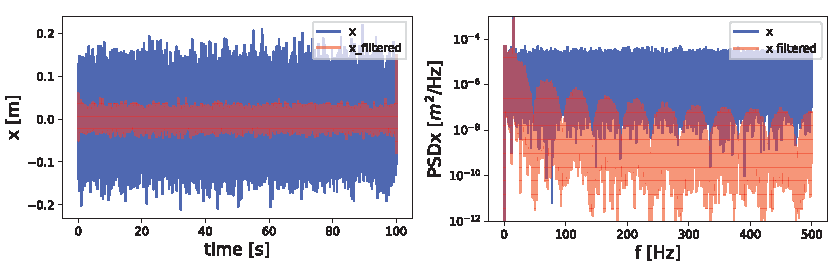
\includegraphics[width=\textwidth]{Figures/psd_fig3.pdf}
        \caption{Beispiel Rauschen und Tiefpassfilter in der PSD. \textbf{Links:} Signal $x(t)$ mit unbekannten Frequenzkomponenten in blau und gefiltertes Signal in rot/ \textbf{Rechts:} PSD von $x(t)$ in blau und vom gefilterten Signal in rot. Die Frequenzkomponente bei 15.75\,Hz ist besonders ausgeprägt und der Tiefpassfilter macht diese Frequenz besser sichtbar.}
        \label{fig:parseval}
\end{figure}

In Abb. \ref{fig:parseval} ist eine Messdatenreihe und ihre PSD zu sehen. Eine Frequenzkomponente bei 15.75\,Hz sticht im Spektrum heraus. Wir können einen \textit{Tiefpassfilter} anwenden, um das Rauschen bei allen anderen Frequenzen zu dämpfen und so das Signal auch im Zeitraum besser sichbar zu machen. 

Wir implementieren einen einfachen digitalen Tiefpassfilter, indem wir jeden Punkt in $x(t)$ mit seinen 10 Nachbarn zu jeder Seite mitteln. Wie erwartet finedne wir, dass die PSD bei höheren Frequenzen deutlich reduziert wurde.\\ 

Nach Gl. (\ref{eq:vl7-9}) wurde durch das Filtern auch die Varianz des Signals verringert, was wir in Abb. \ref{fig:parseval} (links) anhand der Breite des roten gegenüber des blauen Signals qualitativ abschätzen können. \\

%Wenn wir durch das Mitteln verschiedener Frequenzkomponenten interessante Signale verwaschen, können wir stattdessen die Messung auch N Male wiederholen und jeden Punkt als Funktion der Zeit mitteln. 
%In beiden Fällen bilden wir einen Mittelwert und erhalten dementsprechend kleinere Fehler. 
In der gemittelten Messung entspricht jeder Punkt dem Mittelwerts aus mehreren ursprünglichen Messwerten. Dadurch werden die statistischen Fehler an jedem Punkt zu einem Fehler des Mittelwerts, und die Standardabweichung reduziert sich um $1/\sqrt{N}$. Die bedeutet auch, dass benachbarte Punkte (innerhalb der Filterzeit) miteinander korreliert werden, also nicht mehr unabhängige Information enthalten. Dieser Verlust an (hochfrequenten) Informationen ist genau der Effekt, den wir durch das Filtern erzielen wollen. Eine Reduktion des Rauschens geht also automatisch einher mit Informationsverlust.

% \textbf{Beispiel: }
% Sei $x(t)$ eine Timetrace (gemessene Werte als Funktion der Zeit) und $S_{xx}(f)$ die zugehörige PSD definiert zwischen $f=0$ und $f_{max} = 500$\,Hz (``einseitig'', vgl. \cref{subsec:vl7-2}). Falls die PSD ungefähr weiß (``flach'') ist, können wir die Varianz gemäß dem Parseval-Theorem sehr einfach berechnen (vgl. \cref{subsec:vl7-3} und \cref{subsec:vl7-4}):
% \begin{align}
%     \begin{split}
%         \sigma_x^2 &= \Delta_f \sum_{f = 0}^{f_{max}} S_{xx}(f)\\
%         &= \Bar{S}_{xx} f_{max}~,
%     \label{eq:vl10-1}
%     \end{split}
% \end{align}
% Wobei $\Bar{S}_{xx}$ der durchschnittlichen PSD entspricht, siehe Abbildung \textcolor{blue}{take lecture picture}. 
% Daraus sehen wir direkt, dass eine höhere Nyquist-Frequenz $f_{max}$ zu mehr Rauschen führt. Es kann daher von Vorteil sein, eine langsamere Messrate (Samplingrate) zu verwenden, um eine genauere Messung zu erhalten.
    
% \begin{center}
% \textbf{In vielen Situationen gilt die Faustregel: Eine längere und/oder langsamere Messung ist genauer als eine kurze und schnelle Messung.}
% \end{center}


\subsection{Filterarten}
\label{subsec:vl10-2}

Wie in der letzten Sektion gezeigt, kann man Filter einsetzen, um verschiedene Frequenzanteile eines Signals herauszufiltern. Im Wesentlichen unterscheidet man drei Filterarten:
\begin{itemize}
\setlength\itemsep{0em}
    \item Tiefpass (low-pass): Hohe Frequenzanteile werden abgeschw\"acht, niedrige Frequenzanteile werden transmittiert.
    \item Bandpass (band-pass): Frequenzanteile ausserhalb eines bestimmten Frequenzbereiches werden abgeschw\"acht, der Band-Frequenzbereich wird transmittiert.
    \item Hochpass (high-pass): Niedrige Frequenzanteile werden abgeschw\"acht, hohe Frequenzanteile werden transmittiert.
\end{itemize}

\begin{figure}[tbp]
    \centering
        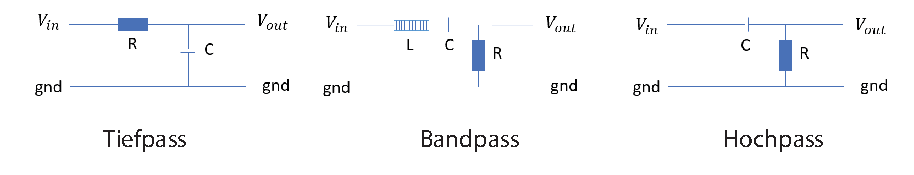
\includegraphics[width=\textwidth]{Figures/filter.pdf}
        \caption{Analoge Implementierung von verschiedenen Filtern. \textbf{Links:} Tiefpass aus paralleler Kapazität \textbf{Mitte:} Bandpass aus serieller Induktivität und Kapazität \textbf{Rechts:} Hochpass aus serieller Kapazität}
        \label{fig:analogueFilters}
\end{figure}

%\textit{Beispiel: Es sei ein Signal mit einer Grundfrequenz von 100\,Hz geben das \"Uberlagerungen h\"oherer und niedriger Frequenzen aufweist (und daher von der Idealform eines Sinus abweicht). Ein Low-pass-Filter mit der Grenzfrequenz $f_{3\,\text{dB}} =$ 150\,Hz schw\"acht alle Frequenzen \"uber 150\,Hz ab, w\"ahrend Frequenzen unterhalb von 150\,Hz mit nahezu maximaler Amplitude durchgelassen werden. Dabei betr\"agt die Abschw\"achung bei 150 Hz 3\,dB. Dadurch wird das urspr\"ungliche Signal entsprechend ``gegl\"attet''. Hingegen transmittiert ein Band-pass-Filter mit $f_{band} =$ 100\,Hz beispielsweise nur einen Frequenzbereich von 50 - 150\,Hz.}\\[0.3 cm]
%Die Ansprechzeit, sprich Wartezeit von Filtern ist direkt proportional zur Frequenz $f$:
% \begin{align}
    %\begin{split}
       % \text{Low-/High-pass: } \tau_{av} &\approx \frac{1}{2 \pi f_{3\,\text{dB}}}\\
        %\text{Band-pass: } \tau_{av} &\approx \frac{1}{\pi f_{3\,\text{dB}}}
        %\label{eq:vl10-3}
    %\end{split}
%\end{align}

Derartige Filter lassen sich digital als Algorithmen oder analog durch elektronische Bauteile implementieren. Die einfachsten analogen, elektronischen Varianten sind, siehe Abb. \ref{fig:analogueFilters}:
\begin{itemize}
\setlength\itemsep{0em}
    \item Low-pass: Widerstand und Kondensator
    \item Band-pass: Spule, Kondensator und Widerstand (ein RLC Resonator)
    \item High-pass: Kondensator und Widerstand
\end{itemize}

Wir betrachten Als Beispiel den typischen RC-Tiefpassfilter, der aus einem Widerstand $R$ in der Signalleitung und einer Kapazität $C$ zur Erdung besteht (siehe Zeichnung in Vorlesungs-Slides). Die Impedanzen (``komplexen Widerst\"ande'') der Elemente $R$ und $C$ sind in Abh\"angigkeit der Signalfrequenz $\omega$ gegeben als:
\begin{align}
    \begin{split}
        Z_R &= R\\
        Z_C &= \frac{1}{i \omega C}\,.
        \label{eq:vl10-4}
    \end{split}
\end{align}

Das Verh\"altnis $T_{filter}$ der Ein- und Ausgangsspannungen $V_{in} = I_{in} (Z_R + Z_C)$ bzw. $V_{out} = I_{in} Z_C$, l\"asst sich wie folgt bestimmen:
\begin{align}
    \begin{split}
        T_{filter} &= \frac{|V_{out}|^2}{|V_{in}|^2}\\
        &= \frac{|Z_C|^2}{|R + Z_C|^2}\\
        &= \frac{1/(\omega C)^2}{R^2 + 1/(\omega C)^2}\\
        &= \frac{1}{1 + (\omega R C)^2}\\
        &= \frac{1}{1 + \omega^2 / \omega_{3\,\text{dB}}^2}\,.
        \label{eq:vl10-5}
    \end{split}
\end{align}

Hierbei ist $\omega_{3\,\text{dB}} = 1/RC$ die Frequenz, bei der $|V_{out}|^2$ den halben Wert von $|V_{in}|^2$ erreicht.\\[0.3 cm]

%Die digitale Implementierung hat folgende Form::
%\begin{itemize}
%\setlength\itemsep{0em}
%    \item Low-pass: $y(n) = x(n) + x(n-1)$ (Fehler des Mittelwerts)
%    \item Band-pass: $y(n) = \underbrace{L_1(n)}_{\text{Low-pass @ } f_1} + %\underbrace{H_2(n)}_{\text{High-pass @ } f_2}$
%    \item High-pass: $y(n) = \underbrace{A(n)}_\text{All-pass} - \underbrace{L(n)}_\text{Low-pass}$
%\end{itemize}


%Es gilt: Reduziere die Unsicherheit (des gemessenen Wertes $S_{xx}$) für jeden Frequenzpunkt durch wiederholte Messungen. Wir erhalten einen ``Fehler des Mittelwertes'' für jeden Wert von $S_{xx} (f)$.

\newpage

\begin{tcolorbox}[enhanced,width=6in,
    fontupper=\small,drop fuzzy shadow southwest,
    colframe=black!50!black,colback=black!5]
\textbf{Verständnisfragen:} \\
\begin{enumerate}
\item[1] Was besagt Fouriers Theorem?
\item[2] Wann würden wir typischerweise die kontinuierliche/diskrete Fouriertransformation benutzen?
\item[3] Was ist die maximale Frequenz, die ohne Aliasing gesampelt werden kann?
\item[4] Was besagt das Parseval-Theorem und warum ist es wichtig? 
\item[5] Wie berechnet man die Standardabweichung $\sigma_x$ eines rauschbehafteten Signals x(t)?
\item[6] Welche Frequenzanteile werden durchgelassen wenn erst ein Hochpass, und dann ein Tiefpassfilter angewendet wird? 
\end{enumerate}
\end{tcolorbox}

\begin{tcolorbox}[enhanced,width=6in,
    fontupper=\small,drop fuzzy shadow southwest,
    colframe=black!50!black,colback=black!5]
\textbf{Antworten:} \\
\begin{enumerate}
\item[1] Fouriers Theorem besagt das jede integrierbare Funtion als Summe von trigonometrischen Funktionen dargestellt werden kann. 
\item[2] Beim Herleiten von analytischen Zusammenhängen verwendet man oft die kontinuierliche Fouriertransformation, und beim analysieren von experimentellen Daten verwendet man im Regelfall die diskrete Fouriertransformation, da eine gespeicherte Messunge aus diskreten Datenpunkten besteht.  
\item[3] Die Nyquist-Frequenz, $f_{max} = 1/2\delta t$
\item[4] Das Parseval-Theorem besagt, dass das Integral über die PSD der Varianz entspricht. Dies ist wichtig zur Normierung der PSD. 
\item[5] Über das Parseval-Theorem lässt sich die Varianz $\sigma_x^2$ aus der PSD berechnen. Die Standardabweichung ist dann $\sqrt{\sigma_x^2}$. 
\item[6] Wenn sich die Frequenzbereiche des Hoch- und Tiefpasses überschneiden, werden diejenigen Frequenzen durchgelassen, die in dem Überschneidungsbereich liegen, ähnlich wie bei einem Bandpass. Wenn sich die Frequenzen der beiden Filter nicht überschneiden, wird kein Signal durchgelassen. 
\end{enumerate}
\end{tcolorbox}
\chapter{Abschätzen von Parametern}
\label{chap:estimation}

\section{Bayessche Datananalyse}
\label{chap:estimation:sec:bayes}

Die Bayessche Analyse präsentiert ein vollkommen anderes Verständnis von Wahrscheinlichkeiten als der frequentistische Ansatz, der in Kapitel \ref{chap:fehler:sec:frequentistisch} behandelt wurde. In diesem Ansatz wird die Unsicherheit als eine subjektive Unsicherheit anstelle einer objektive Unsicherheit des Experiments interpretiert. Während der frequentistische Ansatz eine hohe Anzahl an Wiederholungen eines Experimentes erfordert, um Wahrscheinlichkeiten zu berechnen und aufgrund derer Aussagen über die Zukunft zu treffen, bilden im bayesschen Ansatz subjektive Erfahrungen die Grundlage dafür. Im Fokus der Bayesschen Analyse stehen daher bedingte Wahrscheinlichkeiten und der Satz von Bayes (siehe Gleichung \ref{eq:bayes}) nimmt eine zentrale Stellung ein. Im Folgenden definieren wir
\begingroup
\setlength{\tabcolsep}{10pt} % Default value: 6pt
\renewcommand{\arraystretch}{1.5} % Default value: 1
\begin{table}[H]
\begin{tabular}{l|l}
Die gemessenen Daten des Experiments                                        & $A \rightarrow D$                                 \\
\multirow{2}{*}{\shortstack[l]{Ein endlicher Satz von Ergebnissen, die wir\\
mithilfe der Daten unterscheiden möchten}}                                & \multirow{2}{*}{$B \rightarrow B_1, ..., B_n$} \\
   &       \\
Unser gesamtes zusätzliches Wissen (wird oft vernachlässigt)            & I 
\end{tabular}
\end{table}
\endgroup
und schreiben den Satz von Bayes damit als
\begin{align}
P ( B_i | D, I ) = \frac{ P ( D | B_i, I) P ( B_i | I )}{ P ( D | I ) }\,
\label{eq:bayesrewritten}
\end{align}
oder vereinfacht zu
\begin{align}
P ( B_i | D ) = \frac{ P ( D | B_i) P ( B_i )}{ P ( D ) }\,.
\label{eq:bayesrewrittensimple}
\end{align}
Wenn $D$ impliziert, dass eines der $B_i$ eintritt, gilt weiterhin
\begin{align}
P ( D ) = \sum_k P ( D | B_k ) P ( B_k )\,.
\end{align}

In Gleichung \ref{eq:bayesrewrittensimple} ist $P(B_i)$ die \textit{a-priori} Wahrscheinlichkeit für das Eintreten eines Ergebnisses $B_i$ die auf dem ursprünglichen Wissen \textit{vor} der Durchführung eines Experiments basiert. Es werden nun eine Reihe von Daten $D$ gemessen und die konditionellen Wahrscheinlichkeiten $ P(D|B_i)$ für deren Auftreten in Abhängigkeit des Vorliegens eines bestimmten Ergebnisses $B_i$ berechnet. Die Kenntnis der $P(B_i)$ und $ P(D|B_i)$ ermöglicht es nun, sogenannte \textit{a-posteriori} Wahrscheinlichkeiten $ P(B_i|D)$ zu bestimmen, mit denen ein Ergebnis $B_i$ basierend auf der Grundlage des Datensatzes $D$ auftritt. Es wird also eine subjektive Erfahrung, die Kenntnis des Datensatzes $D$, zur Berechnung der Wahrscheinlichkeiten verwendet.


\begin{center}
\begin{tcolorbox}[enhanced,width=6in,drop fuzzy shadow southwest,
colframe=blue!50!black,colback=blue!01]
\textbf{Beispiel 1}: Die Infektionskrankheit \\
 Nehmen wir an, es gibt eine Infektionskrankheit mit einer Inzidenzrate von 100. Das bedeutet, dass von 100 von 100000 Menschen, also 0.1 \%, infiziert sind.  Die \textit{a-priori} Wahrscheinlichkeiten dafür, ob eine Person infiziert ($B_I$) oder gesund ($B_G$) ist, sind somit
 \begin{align}
 P(B_I) = 0.001 \label{eq:proability-example}
 \end{align}
  \begin{align}
 P(B_G) = 0.999 \label{eq:proability-example2}
 \end{align}
 Eine Person lässt sich nun testen und der Test ist positiv. Wie hoch ist die Wahrscheinlichkeit, dass die Person tatsächlich infiziert ist, wenn der Test in 99\% der Fälle das korrekte Ergebnis liefert?  \\

 Um diese Frage zu beantworten, berechnen wir zuerst die bedingten Wahrscheinlichkeiten
 \begin{align}
P(D|B_I) = 0.99
 \end{align}
  \begin{align}
P(D|B_G) = 0.01
 \end{align}
und verwenden dann den Satz von Bayes. Dieser liefert
\begin{align}
P(B_I|D) = \frac{P(D|B_I)P(B_I)}{P(D|B_I)P(B_I) + P(D|B_G)P(B_G)} = 0.1,
\end{align}
die Wahrscheinlichkeit, dass die Person tatäschlich infiziert ist, liegt somit \glqq nur\grqq  bei 10\%. \\

Wenn sich die Person nun ein weiteres Mal testen lässt und der Test erneut positiv ist, verwenden wir nun die aus dem ersten Testergebnis resultierenden Wahrscheinlichkeiten $P(B_I) = 0.1$ und $P(B_G) = 0.9$ als neue \textit{a-priori} Wahrscheinlichkeiten und verwenden auf dieser Grundlage erneut den Satz von Bayes. Nach der zweiten positiven Testrunde ergibt diese Berechnung, dass die Person zu 92\% infiziert ist. 
\end{tcolorbox}
\end{center}


\begin{center}
\begin{tcolorbox}[enhanced,width=6in, drop fuzzy shadow southwest,
colframe=blue!50!black,colback=blue!01]
\textbf{Beispiel 2}: Das Ziegenproblem \\

Hinter lediglich einem von drei Toren befindet sich eine Ziege. Ziel eines Spiels ist es nun, zu erraten, hinter welchem der Tore sich die Ziege befindet. Der Kandidat des Spiels wird dazu aufgefordert, sich für ein Tor $i=$1, 2 oder 3 zu entscheiden. Anschliessend öffnet der Moderator des Spiels eins der beiden Tore, für das sich der Spieler nicht entschieden hat und hinter dem sich die Ziege \textit{nicht} befindet. Der Kandidat erhält nun die Möglichkeit, entweder auf seiner ursprünglichen Wahl zu bestehen oder seine Meinung nochmals zu ändern. Mit welcher Entscheidung gewinnt er das Spiel mit höherer Wahrscheinlichkeit? \\

Diese Frage lässt sich mithilfe des Satz von Bayes beantworten. Die Wahrscheinlichkeiten $P(B_i)$, das sich die Ziege hinter dem Tor $i$ befindet ist für alle Tore identisch und gleich $\frac{1}{3}$. Nehmen wir nun ein konkretes Szenario an, indem sich der Spieler für ein Tor $k=1$ entscheidet und der Moderator anschliessend das Tor $j=3$ öffnet. Die bedingten Wahrscheinlichkeiten $P(D|B_i)$, dass dieses Ergebnis $D$ eintritt, wenn sich die Ziege hinter einem Tor $i$ befindet, sind somit
\begin{align}
P(D|B_1) = \frac{1}{2} \cdot \frac{1}{3} = \frac{1}{6} 
\end{align}
\begin{align}
P(D|B_2) = 1 \cdot \frac{1}{3} = \frac{1}{3}
\end{align}
\begin{align}
P(D|B_3) = 0 \cdot \frac{1}{3} = 0
\end{align}
Mithilfe des Satzes von Bayes können wir nun die Wahrscheinlichkeiten $P(B_1|D)$ und $P(B_2|D)$ berechnen:
\begin{align}
\begin{split}
P(B_1|D) = \frac{P(D|B_1)P(B_1)}{P(D|B_1)P(B_1) + P(D|B_2)P(B_2) + P(D|B_3)P(B_3)} = \frac{1}{3}
\end{split}
\end{align}

\begin{align}
\begin{split}
P(B_2|D) = \frac{P(D|B_2)P(B_2)}{P(D|B_1)P(B_1) + P(D|B_2)P(B_2) + P(D|B_3)P(B_3)} = \frac{2}{3}
\end{split}
\end{align}
Der Spieler erhöht (verdoppelt) somit seine Gewinnchancen, wenn er seine Wahl nochmals ändert.
\end{tcolorbox}
\end{center}





\section{Likelihood Funktion und Maximum Likelihood}\label{sec:likelihood}

\begin{center}
\begin{tcolorbox}[enhanced,width=6in,center upper,
    fontupper=\large,drop fuzzy shadow southwest,
    colframe=blue!50!black,colback=blue!10]
    {Zur Likelihood Funktion und Maximum Likelihood ist ein Jupyter-Notebook verfügbar. Siehe \gitresource{Likelihood Function.ipynb} }
\end{tcolorbox}
\end{center}

\subsection{Likelihood-Funktion}
\label{subsec:vl8}


Wir haben gesehen, dass eine einzelne Messung äquivalent ist zu einer Ziehung einer Zufallszahl aus einer Wahrscheinlichkeitsverteilung. Die Wahrscheinlichkeitsverteilung einer Zufallsvariable \gls{gl:zeta} sei:
\begin{align}
f(\zeta, a_0, a_1, ..., a_m) = f (\zeta, \boldsymbol{a})\,.
\label{eq:vl8-1}
\end{align}

Hierbei ist $\boldsymbol{a}$ ein Vektor der die Wahrscheinlichkeitsverteilung parametrisiert, wie z. B. in Gl. (\ref{eq:proability-example}) und (\ref{eq:proability-example2}). F\"ur mehrere Variablen schreiben wir: 
\begin{align}
f(\zeta_0, \zeta_1, ..., \zeta_n, a_0, a_1, ..., a_m) = f (\boldsymbol{\zeta}, \boldsymbol{a}).\,
\label{eq:vl8-2}
\end{align}

In einem Experiment sind die Werte der $a_i$ unbekannt, aber wir kennen (aus der Messung) einige $\zeta_i$, zum Beispiel messen wir die Werte $\zeta_i = x_i$. Also k\"onnen wir schreiben:
\begin{align}
f(x_0, x_1, ..., x_n, \boldsymbol{a}) = f(\boldsymbol{x, a}) \overset{\text{def}}{=} L (\boldsymbol{x,a})\,.
\label{eq:vl8-3}
\end{align}

\begin{center}
\begin{tcolorbox}[enhanced,width=6in,drop fuzzy shadow southwest,
    colframe=red!50!black,colback=red!05]
   Hierbei ist $L$ die Likelihood-Funktion. In der Likelihood-Funktion sind die $x_i$ bekannt und die $a_i$ sind die Variablen.
\end{tcolorbox}
\end{center}


\textit{Beispiel: Wir messen zwei unabh\"angige Datenpunkte $x_1$ und $x_2$ aus einer Gaussverteilung:}
\begin{align}
f(\zeta, a_0, a_1) = \frac{1}{ \sqrt{ 2 \pi a_1 } } \exp \left( - \frac{1}{2} \frac{ (\zeta - a_0)^2 }{ a_1 } \right)\,.
\label{eq:vl8-4}
\end{align}

\textit{Die Parameter $a_0$ (der Erwartungswert) und $a_1$ (die Varianz) sind unbekannt. Da die Messungen unabh\"angig sind, ist die gemeinsame Wahrscheinlichkeitsverteilung das Produkt der Einzelwahrscheinlichkeiten:}
\begin{align}
f(x_1, x_2, a_0, a_1) &= f(x_1, a_0, a_1)f(x_2, a_0, a_1) = \frac{1}{ 2 \pi a_1 } \exp \left( - \frac{1}{2} \frac{ \sum_{i=1}^2 (x_i - a_0)^2 }{ a_1 } \right)\,. \\
L(x_1, x_2, a_0, a_1) &= f(x_1, x_2, a_0, a_1)
\label{eq:vl8-5}
\end{align}

In diesem Beispiel sieht die Likelihood-Funktion der Wahrscheinlichkeitsverteilung sehr \"ahnlich. Aber Vorsicht:

\begin{center}
\begin{tcolorbox}[enhanced,width=6in,drop fuzzy shadow southwest,
    colframe=red!50!black,colback=red!05]
   Die Likelihood-Funktion ist \textbf{keine} Wahrscheinlichkeitsverteilung. Die Likelihood-Funktion ist eine Plausibilitätsfunktion.
\end{tcolorbox}
\end{center}

Insbesondere ist sie nicht normiert.\\[0.3cm]
\textit{Beispiel: Wir haben einen Satz von Widerst\"anden mit einer unbekannten Toleranz, wie in Abb. \ref{fig:likelihood}, links als Histogramm gezeigt.
Wir nehmen an, dass die Widerstandswerte normalverteilt sind. F\"ur $n$ Datenpunkte $\boldsymbol{x} = (x_1, x_2, ..., x_n)$ gilt dann:}
\begin{align}
L(\boldsymbol{x}, a_0, a_1) =  \prod_{i = 1}^n f(x_i, a_0, a_1) = \left( \frac{1}{ 2 \pi a_1 } \right)^\frac{n}{2} \exp \left( - \frac{1}{2} \frac{ \sum_{i=1}^n (x_i - a_0)^2 }{ a_1 } \right)\,.
\label{eq:vl8-6}
\end{align}

\begin{figure}[tbp]
    \centering
        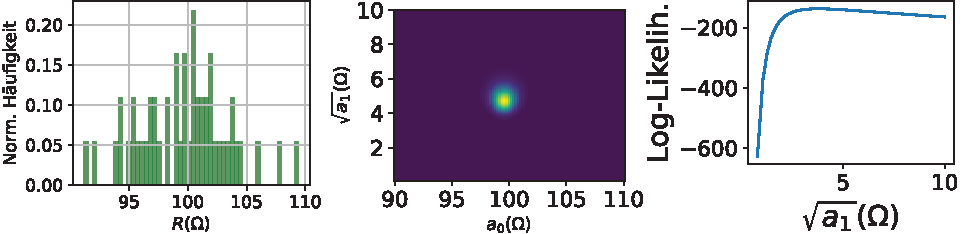
\includegraphics[width=0.8\textwidth]{Figures/likelihood_funktion.pdf}
        \caption{Beispiel zur Likelihood Funktion \textbf{Links:} Histogramm von "gemessenen" Widerstandswerten. \textbf{Mitte:} Likelihood Funktion für verschiedene Parameter $a_{0,1}$ der zugrunde liegendenden Normalverteilung. \textbf{Rechts:} Log-Likelihood Funktion der gleichen Daten. }
        \label{fig:likelihood}
\end{figure} 

\textit{Wir berechnen die Likelihood-Funktion f\"ur ``alle'' Werte von $a_0$ und $a_1$. 
Das Ergebnis ist in Abb. \ref{fig:likelihood}, Mitte zu sehen. 
Wir finden die maximale Likelihood f\"ur eine Verteilung bei $\hat{a}_0 = 100\,\Omega$ und $\sqrt{\hat{a}_1} = 5\,\Omega$.\\
In diesem Fall, weil die Daten normalverteilt sind, h\"atten wir auch die Ausdr\"ucke f\"ur die Absch\"atzung von Erwartungswert und Standardabweichung benutzen k\"onnen. Aber die Analyse der Likelihood-Funktion funktioniert auch bei beliebigen anderen Verteilungen.}


\subsection{Maximum Likelihood}
\label{subsec:vl8-2}

Der genaue Wert der Likelihood-Funktion ist nicht besonders aussagekr\"aftig. Weil sie nicht normiert sein muss, gibt sie uns keine Wahrscheinlichkeit bzw. Wahrscheinlichkeitsdichte. Aber die Likelihood-Funktion beinhaltet Information \"uber die Parameter $\boldsymbol{a}$ der Wahrscheinlichkeitsverteilung. Sie gibt uns eine Plausibilität für die Werte der Parameter $\boldsymbol{a}$. Daher sind Werte von $\boldsymbol{a}$, die eine grosse Likelihood haben, zu bevorzugen.\\[0.3cm]
Wir k\"onnen Likelihoods \"uber ihr Verh\"altnis vergleichen:
\begin{align}
LR = \frac{L(\boldsymbol{x,a})}{L(\boldsymbol{x,b})}\,.
\label{eq:vl8-7}
\end{align}

Dies ist das Verh\"altnis der ``Plausibilitäten'', dass die Parameter $\boldsymbol{a}$ und $\boldsymbol{b}$ die gemessenen Daten erkl\"aren. Insbesondere wollen wir die Werte f\"ur $\boldsymbol{a}$ finden, die die Likelihood-Funktion maximieren.

\begin{center}
\begin{tcolorbox}[enhanced,width=6in,drop fuzzy shadow southwest,
    colframe=red!50!black,colback=red!05]
   Dies ist das sogenannte \textbf{Maximum Likelihood}-Prinzip. 
\end{tcolorbox}
\end{center}


Wir beginnen wieder mit gaussverteilten Daten $\boldsymbol{x} = (x_1, x_2, ..., x_n)$. Die zugrundeliegende Likelihood-Funktion ist:
\begin{align}
f(\zeta, a_0, a_1) = \frac{1}{ \sqrt{2 \pi a_1} } \exp \left( - \frac{1}{2} \frac{ (\zeta - a_0)^2 }{ a_1 } \right)\,.
\label{eq:vl8-8}
\end{align}

Die Parameter $a_0$ (der Erwartungswert) und $a_1$ (die Varianz) sind wieder unbekannt und wir wollen diese Werte absch\"atzen. Die kombinierte Likelihood-Funktion ist dann das Produkt der einzelnen Likelihood-Funktionen:
\begin{align}
L(\boldsymbol{x}, a_0, a_1) =  \left( \frac{1}{ 2 \pi a_1 } \right)^\frac{n}{2} \exp \left( - \frac{1}{2} \frac{ \sum_{i=1}^n (x_i - a_0)^2 }{ a_1 } \right)\,.
\label{eq:vl8-9}
\end{align}

Wir sind ausschliesslich an den Werten von $a_0$, $a_1$ interessiert die diese Funktionen maximieren, aber nicht am Wert des Maximums. Wir k\"onnen also den Logarithmus nehmen (Damit l\"asst sich leichter rechnen.):
\begin{align}
\gls{gl:logl}(x, a_0, a_1) = - \frac{n}{2} \ln{ ( 2 \pi a_1 ) } - \frac{1}{2} \frac{ \sum_{i=1}^n (x_i - a_0)^2 }{ a_1 }\,.
\label{eq:vl8-10}
\end{align}

\begin{center}
\begin{tcolorbox}[enhanced,width=6in,drop fuzzy shadow southwest,
    colframe=red!50!black,colback=red!05]
   Dies ist die sogenannte \textbf{Log-Likelihood-Funktion. }
\end{tcolorbox}
\end{center}

In Abb. \ref{fig:likelihood}, rechts, ist die Log-Likelihood Funktion für das Beispiel im vorigen Abschnitt zu sehen. \\

Wir wollen also die Log-Likelihood-Funktion (\cref{eq:vl8-10}) maximieren. Also berechnen wir die Ableitung von $l$ nach $a_0$ und $a_1$ an dem Stellen $\hat{a}_0$ und $\hat{a}_1$ und setzen diese gleich Null, sodass $\hat{a}_0$ und $\hat{a}_1$ dann die Werte sind, die $l$ maximieren:
\begin{align}
\begin{split}
\frac{ \partial l }{ \partial a_0 } &= \frac{ \partial }{ \partial a_0 } \bigg|_{\hat{a}_0, \hat{a}_1} - \frac{n}{2} \ln{ ( 2 \pi a_1 ) } - \frac{1}{2} \frac{ \sum_{i=1}^n (x_i - a_0)^2 }{ a_1 } = 0\,,\\
\rightarrow 0 &= \frac{1}{ \hat{a}_1} \sum_{i = 1}^n (x_i - \hat{a}_0)\,,\\
&=  \frac{1}{ \hat{a}_1} \left( \sum_{i = 1}^n x_i - n \hat{a}_0 \right)\\
\text{Der Erwartungswert:}\quad \quad \rightarrow \hat{a}_0 &= \frac{1}{n} \sum_{i = 1}^n x_i\\
\label{eq:vl8-11}
\end{split}
\end{align}
und:
\begin{align}
\begin{split}
\frac{ \partial l }{ \partial a_1 } &= \frac{ \partial }{ \partial a_1 } \bigg|_{\hat{a}_0, \hat{a}_1} - \frac{n}{2} \ln{ ( 2 \pi a_1 ) } - \frac{1}{2} \frac{ \sum_{i=1}^n (x_i - a_0)^2 }{ a_1 } = 0\,,\\
\rightarrow 0 &= - \frac{n}{2}\frac{1}{ \hat{a}_1 } + \frac{1}{ 2 \hat{a}_1^2 }\sum_{i = 1}^n (x_i - \hat{a}_0)^2\,,\\
\text{Die Varianz:}\quad \quad \quad \quad \quad \enspace
\rightarrow \hat{a}_1 &= \frac{1}{n} \sum_{i = 1}^n (x_i - \hat{a}_0)^2\,.
\label{eq:vl8-12}
\end{split}
\end{align}

Bemerkung: Der Wert der Varianz hat einen Bias im Vergleich zu dem Wert f\"ur die empirische Varianz.


\subsection{Der gewichtete Mittelwert}
\label{subsec:vl8-3}

Wir betrachten nun ein h\"aufiges Szenario. Wir messen mit einer uns bekannten und charakterisierten Messapparatur. Das heisst die Messunsicherheit (die Standardabweichung) $\sigma_i$ jeder Messung ist bekannt. Wir messen den Datensatz $\boldsymbol{x} = (x_1, x_2, ..., x_n)$ und wollen den Mittelwert bestimmen.\\
Die zugrundeliegende Likelihood-Funktion jeder Messung ist:
\begin{align}
f_i(\zeta_i, \sigma_i, a) = \frac{1}{ \sqrt{2 \pi } \sigma_i} \exp \left( - \frac{1}{2} \frac{ (\zeta - a)^2 }{ \sigma_1^2 } \right)\,.
\label{eq:vl8-13}
\end{align}

Damit is die Likelihood-Funktion:
\begin{align}
L(\boldsymbol{x,\sigma}, a) = \prod_{i=1}^n \frac{1}{ \sqrt{2 \pi } \sigma_i} \exp \left( - \frac{1}{2} \frac{ (x_i - a)^2 }{ \sigma_i^2 } \right)
\label{eq:vl8-14}
\end{align}

und die Log-Likelihood-Funktion:
\begin{align}
l(x,\sigma, a) = \sum_{i=1}^n \ln \left( \frac{1}{ \sqrt{2 \pi } \sigma_i} \right) - \frac{1}{2} \sum_{i=1}^n \frac{ (x_i - a)^2 }{ \sigma_i^2 }\,.
\label{eq:vl8-15}
\end{align}

Wir bestimmen das Maximum:
\begin{align}
\begin{split}
\frac{ \partial l }{ \partial a } \bigg|_{\hat{a}} &= \frac{ \partial }{ \partial a } \bigg|_{\hat{a}} \left( - \frac{1}{2} \sum_{i=1}^n \frac{ (x_i - a)^2 }{ \sigma_i^2 } \right) = 0\,,\\
\rightarrow \sum_{i=1}^n \frac{ x_i - \hat{a} }{ \sigma_i^2 } &=  \sum_{i=1}^n \frac{ x_i }{ \sigma_i^2 } - \hat{a} \sum_{i=1}^n \frac{ 1 }{ \sigma_i^2 }\,,\\
\rightarrow \hat{a} &= \frac{ \sum_{i=1}^n \frac{ x_i }{ \sigma_i^2 } }{ \sum_{i=1}^n \frac{ 1 }{ \sigma_i^2 } } =\frac{ \sum_{i=1}^n w_i x_i }{ \sum_{i=1}^n w_i \,}.
\label{eq:vl8-16}
\end{split}
\end{align}

Hier definieren wir das Gewicht der einzelnen Messwerte als $w_i = \frac{1}{\sigma_i^2}$. 
Letzteres ist der \textbf{gewichtete Mittelwert}. Das heisst die Einzelnen Werte $x_i$ tragen zum Wert des Mittelwertes mehr bei, wenn sie eine kleinere Unsicherheit haben. Werte mit grosser Unsicherheit haben dementsprechend einen kleineren Beitrag zum Mittelwert.



\chapter{Fitten von Parametern}
 
\section{Lineares Fitten von Polynomen}
\begin{center}
\begin{tcolorbox}[enhanced,width=6in,center upper,
    fontupper=\large,drop fuzzy shadow southwest,
    colframe=blue!50!black,colback=blue!10]
    {Zum linearen Fitten ist ein Jupyter-Notebook verfügbar. Siehe \gitresource{linear\_fitting.ipynb} }
\end{tcolorbox}
\end{center}

\subsection{Die Methode der kleinsten Quadrate}
\label{subsec:vl8-4}

Bisher haben wir die Likelihood-Funktion maximiert, um Parameter zu bestimmen, die die Wahrscheinlichkeitsverteilung (PDF) eines Datensatzes beschreiben. Insbesondere die Log-Likelihood-Funktion ist einfach zu maximieren wenn die PDF eine Gaussverteilung ist:
\begin{align}
\frac{ \partial l }{ \partial a } \bigg|_{\hat{a}} &= \frac{ \partial }{ \partial a } \bigg|_{\hat{a}} \left( - \frac{1}{2} \sum_{i=1}^n \frac{ (x_i - a)^2 }{ \sigma_i^2 } \right) = 0\,.
\label{eq:vl8-17}
\end{align}

In diesem Fall ist die Maximierung der Log-Likelihood-Funktion \"aquivalent zur Minimierung der Summer der  Abstandsquadrate der einzelnen Messpunkte zum Erwartungswert (also dem Modell). Dies ist die Methode der kleinsten Quadrate.
Wir definieren die Summer der Abstandsquadrate $S = \sum_{i=1}^n \frac{ (x_i - a)^2 }{ \sigma_i^2 }$ und damit schreiben wir:
\begin{align}
\frac{ \partial S }{ \partial a } \bigg|_{\hat{a}} &= \frac{ \partial }{ \partial a } \bigg|_{\hat{a}} \sum_{i=1}^n \frac{ (x_i - a)^2 }{ \sigma_i^2 } = 0\,.
\label{eq:vl8-18}
\end{align}

Bemerkung: Wenn die $\sigma_i$ bekannt sind, dann ist dies \"aquivalent zur Minimierung von $\chi^2$ und damit ist $S = \chi^2$. Das ist jedoch oft nicht der Fall, wir bleiben also zun\"achst bei $S$.


\subsection{Lineares Fitten von Polynomen}
\label{subsec:vl8-5}

\begin{figure}[tbp]
    \centering
        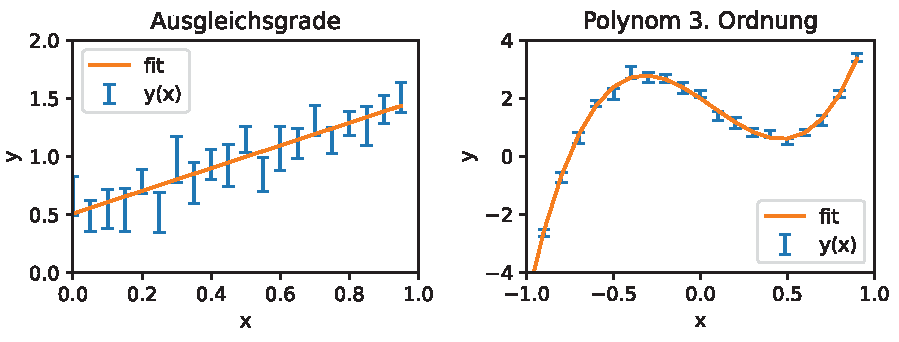
\includegraphics[width=0.8\textwidth]{Figures/linear_fitting_image.pdf}
        \caption{Beispiel zum linearen Fitten. \textbf{Links:} Linearer Fit einer Ausgleichsgrade zu fehlerbehafteten Daten. \textbf{Rechts:} Linearer Fit eines Polynoms dritter Ordnung zu fehlerbehafteten Daten. }
        \label{fig:linearFit}
\end{figure} 

\subsubsection{Fitten einer Ausgleichsgeraden}
\label{subsubsec:vl8}

Wir haben die Werte $y_1, y_2, ..., y_n$ als Funktion der Kontrollparameter $x_1, x_2, ..., x_n$ gemessen. Die $x_i$ haben keine Unsicherheit, w\"ahrend die Unsicherheiten der $y_i$ durch $\sigma_i$ gegeben sind. Das bedeutet, dass die Wahrscheinlichkeit, dass der Wert $y$ gemessen wird gegeben ist durch:
\begin{align}
f(y) \sim \exp \left( - \frac{ (y - \mu)^2 }{ 2 \sigma^2 } \right)\,,
\label{eq:vl8-19}
\end{align}

wobei beide Werte $y$ und $\sigma$ von $x$ abh\"angen. Wir nehmen an, dass $\mu = a_0 + a_1 x$, also dass die Erwartungswerte von $y$ linear von $x$ abh\"angen, wie in Abb. \ref{fig:linearFit}, links zu sehen ist. Wir wollen die Werte von $a_0$ und $a_1$ finden, die die Daten am besten wiedergeben. Das heisst:
\begin{align}
f(y) \sim \exp \left( - \frac{ (y - a_0 - a_1 x_i)^2 }{ 2 \sigma_i^2 } \right)
\label{eq:vl8-20}
\end{align}

ist die Wahrscheinlichkeitsverteilung der $y_i$. Dann ist die Likelihood-Funktion f\"ur den $i-$ten Datenpunkt:
\begin{align}
L(x_i, y_i, \sigma_i, a_0, a_1) \sim \exp \left( - \frac{ (y_i - a_0 - a_1 x_i)^2 }{ 2 \sigma_i^2 } \right)
\label{eq:vl8-21}
\end{align}

und die kombinierte Log-Likelihood-Funktion für alle Datenpunkte:
\begin{align}
l(\boldsymbol{x, y, \sigma}, a_0, a_1) = - \frac{1}{2} \sum_{i=1}^n \frac{ (y_i - a_0 - a_1 x_i)^2 }{ \sigma_i^2 } + C
\label{eq:vl8-22}
\end{align}

mit einer Konstanten $C$. Wir benutzen wieder die Gewichte $w_i= \frac{1}{\sigma_i^2}$ und damit ist:
\begin{align}
l(\boldsymbol{x, y, w}, a_0, a_1) = - \frac{1}{2} \sum_{i=1}^n w_i (y_i - a_0 - a_1 x_i)^2 + C\,.
\label{eq:vl8-23}
\end{align}

Wir k\"onnen die besten Absch\"atzungen f\"ur $a_0$ und $a_1$ finden, indem wir die partiellen Ableitungen von $l$ nach $a_0$ und $a_1$ gleich Null setzen. Da die Unsicherheiten einer Normalverteilung zugrunde liegen, k\"onnen wir auch die gewichtete Summe der Abstandsquadrate (der Residuen) minimieren:
\begin{align}
S  = \sum_{i=1}^n w_i (y_i - a_0 - a_1 x_i)^2\,.
\label{eq:vl8-24}
\end{align}

\begin{center}
\begin{tcolorbox}[enhanced,width=6in,drop fuzzy shadow southwest,
    colframe=red!50!black,colback=red!05]
   Die Residuen sind die Abst\"ande der gemessenen Datenpunkte vom Modell.
\end{tcolorbox}
\end{center}

Wir haben also zwei Gleichungen:
\begin{align}
\begin{split}
\frac{ \partial S }{ \partial a_0 } &= - 2 \sum_{i = 1}^n w_i (y_i - \hat{a}_0 - \hat{a}_1 x_i) = 0\,,\\
\frac{ \partial S }{ \partial a_1 } &= - 2 \sum_{i = 1}^n w_i x_i (y_i - \hat{a}_0 - \hat{a}_1 x_i) = 0\,,
\label{eq:vl8-25}
\end{split}
\end{align}

mit den L\"osungen:
\begin{align}
\begin{split}
\hat{a}_0 &= \frac{ \sum w_i x_i^2 \sum w_i y_i - \sum w_i x_i \sum w_i x_i y_i }{ \sum w_i \sum w_i x_i^2 - (\sum w_i x_i)^2 }\,,\\
\hat{a}_1 &= \frac{ \sum w_i \sum w_i x_i y_i - \sum w_i x_i \sum w_i y_i }{ \sum w_i \sum w_i x_i^2 - (\sum w_i x_i)^2 }\,.
\label{eq:vl8-26}
\end{split}
\end{align}

Wir k\"onnen das auch in Matrixform schreiben (die sogenannte Normalform):
\begin{align}
\begin{pmatrix}
\sum w_i     & \sum w_i x_i   \\
\sum w_i x_i & \sum w_i x_i^2
\end{pmatrix}
\begin{pmatrix}
\hat{a}_0 \\
\hat{a}_1
\end{pmatrix}
&= 
\begin{pmatrix}
\sum w_i y_i \\
\sum w_i x_i y_i
\end{pmatrix}\,,\\
\intertext{}
\boldsymbol{N \hat{a}} = \boldsymbol{Y}\,,
\label{eq:vl8-28}
\end{align}

mit der L\"osung:
\begin{align}
\boldsymbol{\hat{a}} = \boldsymbol{N^{-1} Y}\,.    
\label{eq:vl8-28-2}
\end{align}

In Abb. \ref{fig:linearFit}, links, ist ein fehlerbehafteter Datensatz $y(x)$ zu sehen, der einer linearen Funktion folgt. 
Minimieren der Abstandsquadrate ergibt eine Auslgleichsgerade, die die Datenpunkte beschreibt. 

\subsubsection{Fitten eines Polynoms \texorpdfstring{$m$}{m}-ter Ordnung}
\label{subsubsec:vl8-2}

Dies kann nun sehr einfach auf Polynome beliebiger Ordnung erweitert werden: $y = a_0 + a_1 x + a_2 x^2 + ... + a_m x^m$ und hat dann folgende explizite Form:
\begin{align}
\begin{pmatrix}
\sum w_i       & \sum w_i x_i       & \cdots & \sum w_i x_i^m     \\
\sum w_i x_i   & \sum w_i x_i^2     & \cdots & \sum w_i x_i^{m+1} \\
\vdots         & \vdots             & \ddots & \vdots             \\
\sum w_i x_i^m & \sum w_i x_i^{m+1} & \cdots & \sum w_i x_i^{2m}  
\end{pmatrix}
&
\begin{pmatrix}
\hat{a}_0 \\
\hat{a}_1 \\
\vdots    \\
\hat{a}_m
\end{pmatrix}
= 
\begin{pmatrix}
\sum w_i y_i       \\
\sum w_i x_i y_i   \\
\vdots             \\
\sum w_i x_i^m y_i
\end{pmatrix}\,,\\
\intertext{}
\boldsymbol{N \hat{a}} = \boldsymbol{Y}\,,
\label{eq:vl8-29}
\end{align}

ebenfalls mit der L\"osung:
\begin{align}
\boldsymbol{\hat{a}} = \boldsymbol{N^{-1} Y}\, ,    
\label{eq:vl8-29-2}
\end{align}
was für $m=3$ in Abb. \ref{fig:linearFit}, rechts dargestellt ist. 


\begin{center}
\begin{tcolorbox}[enhanced,width=6in,drop fuzzy shadow southwest,
    colframe=red!50!black,colback=red!05]
   Diese Methode wird Lineares Fitten genannt, weil das Gleichungssystem in Gl. (\ref{eq:vl8-29}) ein lineares Gleichungssystem ist, nicht nur wenn man eine Augleichsgerade fittet. 
\end{tcolorbox}
\end{center}

\subsubsection{Unsicherheiten der Fitparameter}
\label{subsubsec:vl8-3}

Auf diese Weise k\"onnen wir analytisch die beste Absch\"atzung der Modellparameter $\boldsymbol{a}$ bestimmen. Aber wir wollen auch wissen wie zuverl\"assig diese Werte sind; wir m\"ochten \textbf{Varianz} und \textbf{Kovarianz} wissen. Das Polynom berechnet mit den $\hat{a}$, wird nicht durch alle Datenpunkte gehen. Also k\"onnen wir schreiben:
\begin{align}
y_i = \hat{a}_0 + \hat{a}_1 x_i + ... + \hat{a}_m x_i^m + \epsilon_i\,,
\label{eq:vl8-30}
\end{align}

wobei \gls{gl:epsilon}$_i$ der Abstand ist, den der $i$-te Punkt von der gefitteten Funktion hat: \textbf{Die Residuen}. Wir nehmen an, dass die Unsicherheiten der $y_i$ durch zuf\"allige Fehler zustande kommen und normalverteilt sind. Dann sind die $\epsilon_i$ unkorreliert und ihr Erwartungswert ist Null:
\begin{align}
\langle \epsilon_i \rangle = 0 \quad \langle \epsilon_i, \epsilon_j \rangle = \sigma_i^2 \delta_{ij}\,.
\label{eq:vl8-31}
\end{align}

Wir definieren die Vektoren:
\begin{align}
\boldsymbol{y} = 
\begin{pmatrix}
y_1    \\
y_2    \\
\vdots \\
y_n
\end{pmatrix}\quad
\boldsymbol{\epsilon} = 
\begin{pmatrix}
\epsilon_1 \\
\epsilon_2 \\
\vdots     \\
\epsilon_n
\end{pmatrix}\quad
\boldsymbol{a} = 
\begin{pmatrix}
a_1    \\
a_2    \\
\vdots \\
a_n
\end{pmatrix}\,
\label{eq:vl8-32}
\end{align}

und die Matrizen:
\begin{align}
\boldsymbol{X} = 
\begin{pmatrix}
1      & x_1    & \cdots & x_1^m  \\
1      & x_2    & \cdots & x_2^m  \\
\vdots & \vdots & \ddots & \vdots \\
1      & x_n    & \cdots & x_n^m  \\
\end{pmatrix}\quad
\boldsymbol{W} = 
\begin{pmatrix}
w_1    & \cdots & \cdots & 0      \\
\vdots & w_2    & \cdots & \vdots \\
\vdots & \vdots & \ddots & \vdots \\
0      & \cdots & \cdots & w_n    \\
\end{pmatrix}\,.
\label{eq:vl8-33}
\end{align}

Damit wird \cref{eq:vl8-30} zu:
\begin{align}
\boldsymbol{y} = \boldsymbol{X} \boldsymbol{a} + \boldsymbol{\epsilon}\,.
\label{eq:vl8-34}
\end{align}

Wir k\"onnen wieder die Normalmatrix und den gewichteten Ergebnisvektor finden:
\begin{align}
\boldsymbol{N} = \boldsymbol{X}^T \boldsymbol{W X} \quad \text{und} \quad \boldsymbol{Y} = \boldsymbol{X}^T \boldsymbol{W y}\,.
\label{eq:vl8-35}
\end{align}

Der Ausdruck f\"ur $S$, die gewichtete Summe der Quadrate der Residuen ist dann:
\begin{align}
S = ( \boldsymbol{y} - \boldsymbol{ X a } )^T \boldsymbol{W}( \boldsymbol{y} - \boldsymbol{X a )}\,.
\label{eq:vl8-36}
\end{align}

Die Normalform hat folgende Gestalt:
\begin{align}
( \boldsymbol{X}^T \boldsymbol{WX} ) \boldsymbol{a} = ( \boldsymbol{X}^T \boldsymbol{Wy} )
\label{eq:vl8-37}
\end{align}

mit der L\"osung:
\begin{align}
\boldsymbol{\hat{a}} = ( \boldsymbol{X}^T \boldsymbol{WX} )^{-1} \boldsymbol{X}^T \boldsymbol{Wy}\,.
\label{eq:vl8-38}
\end{align}

Die Unsicherheiten der Parameter $\boldsymbol{\hat{a}}$ sind gegeben durch deren Varianz:
\begin{align}
\hat{\sigma}_i^2 = \langle ( \hat{a}_i - a_i )^2 \rangle
\label{eq:vl8-39}
\end{align}

und Kovarianz:
\begin{align}
\hat{\sigma}_{ij}^2 = \langle ( \hat{a}_i - a_j ) ( \hat{a}_j - a_i ) \rangle
\label{eq:vl8-40}
\end{align}

relativ zu den (unbekannten) tats\"achlichen Werten $\boldsymbol{a}$. Das k\"onnen wir auch als Matrix schreiben, in der Kovarianzmatrix:
\begin{align}
\boldsymbol{C} = 
\begin{pmatrix}
\hat{\sigma}_i^2  & \cdots & \hat{\sigma}_{0m}^2 \\
\vdots            & \ddots & \vdots            \\
\hat{\sigma}_{m0}^2 & \cdots & \hat{\sigma}_m^2  
\end{pmatrix}
= \langle ( \boldsymbol{\hat{a}} - \boldsymbol{a} )( \boldsymbol{\hat{a}} - \boldsymbol{a} )^T \rangle \,.
\label{eq:vl8-41}
\end{align}

Mit den Ausdr\"ucken und Definitionen die wir eingef\"uhrt haben finden wir:
\begin{align}
\boldsymbol{C} = \left\langle \left( ( \boldsymbol{X}^T \boldsymbol{WX} )^{-1} \boldsymbol{X}^T \boldsymbol{W \epsilon} \right) \left( ( \boldsymbol{X}^T \boldsymbol{WX} )^{-1} \boldsymbol{X}^T \boldsymbol{W \epsilon} \right)^T \right\rangle 
\label{eq:vl8-42}
\end{align}

und mit $\langle \boldsymbol{ \epsilon \epsilon}^T \rangle  = \boldsymbol{W}^{-1} $ wird das zu:
\begin{align}
\boldsymbol{C} = ( \boldsymbol{X}^T \boldsymbol{WX} )^{-1} = \boldsymbol{N}^{-1}\,.
\label{eq:vl8-43}
\end{align}

Bemerkung: Tat\"achlich sind die $\sigma_i$ nicht gut genug bekannt. Das heisst $\sigma_i \neq \langle \epsilon_i^2 \rangle$. Das kann korrigiert werden und man findet nach langer Rechnung:
\begin{align}
\boldsymbol{C} = \frac{ \hat{S}_\text{min} }{ n - m -1 } \boldsymbol{N}^{-1}\,.
\label{eq:vl8-44}
\end{align}

Hierbei ist $\hat{S}_\text{min} = \sum_{i=1}^n w_i ( y_i - \hat{a}_0 - \hat{a}_1 x_i - ... \hat{a}_m x_i^m)^2$, der minimale Wert von $S$ ausgewertet f\"ur die Werte von $\boldsymbol{\hat{a}}$.


\subsection{Zusammenfassung}
\label{subsec:vl8-6}

\begin{itemize}
    \setlength\itemsep{0em}
        \item Wahrscheinlichkeitsverteilungen beschreiben die Wahrscheinlichkeiten von m\"oglichen Ergebnissen von Zufallsexperimenten.
        \item Wir maximieren die (Log-)Likelihood-Funktion um die wahrscheinlichsten Werte f\"ur die Parameter der Wahrscheinlichkeitsverteilung zu finden.
        \item Die Likelihood-Funktion ist nicht normiert und somit selbst keine Wahrscheinlichkeitsverteilung.
        \item Wir k\"onnen Polynome $m$-ter Ordnung fitten, indem wir die Normalmatrix $\boldsymbol{N}$ berechnen.
        \item Die Unsicherheit (Varianz und Kovarianz) der Fitparameter ist gegeben durch die Kovarianzmatrix $\boldsymbol{C} = \boldsymbol{N}^{-1}$.
\end{itemize}

\section{Fitten von nichtlinearen Funktionen}\label{sec:nonLinearFit}
\begin{center}
\begin{tcolorbox}[enhanced,width=6in,center upper,
    fontupper=\large,drop fuzzy shadow southwest,
    colframe=blue!50!black,colback=blue!10]
    {Zum nichtlinearen Fitten ist ein Jupyter-Notebook verfügbar. Siehe \gitresource{nonlinear\_fitting.ipynb} }
\end{tcolorbox}
\end{center}

\subsection{Nichtlineare Sch\"atzung der kleinsten Quadrate}
\label{subsec:vl9}

Um die lineare Funktion $a_0 - a_1 x_i$ an einen gemessen Datensatz $y_1, y_2, ..., y_n$, gemessen als Funktion der unabh\"angigen Variable $x_1, x_2, ..., x_n$ zu fitten, haben wir die Summe der Abstandsquadrate (Residuen) minimiert, vgl. \cref{eq:vl8-24}. Im Allgemeinen heisst das also f\"ur eine Funktion $f(x, a_0, a_1, ..., a_m) = f(x, \boldsymbol{a})$ wir m\"ussen
\begin{align}
S = \sum_{i=1}^n w_i (y_i - f(x_i, \boldsymbol{a}) )^2
\label{eq:vl9-1}
\end{align}

minimieren. Wir k\"onnen nun $S$ als Funktion von ``allen'' $\boldsymbol{a}$ berechnen. Das ergibt uns eine Fl\"ache im $m + 2$ dimensionalen Raum.


\begin{center}
\begin{tcolorbox}[enhanced,width=6in,drop fuzzy shadow southwest,
    colframe=red!50!black,colback=red!05]
   Das Ziel ist nun das Minimum von $S$ zu finden. Da es im Allgemeinen keine geschlossene L\"osung gibt, sind iterative Ans\"atze notwendig.
\end{tcolorbox}
\end{center}


\subsubsection{Gradientenverfahren}
\label{subsubsec:vl9-1}

Wir starten mit einer initialen Sch\"atzung der Werte von $\boldsymbol{a}$: $\boldsymbol{a}_\mathrm{g}$ und bewegen uns auf der Fl\"ache $S$ entlang des steilsten Gradienten den wir aus der Linearisierung (Taylor-Entwicklung erster Ordnung) erhalten. Dieser Methode folgen wir iterativ zum Minimum von $S$:
\begin{align}
S \approx S(\boldsymbol{a}_\mathrm{g}) + \sum_{i=0}^m \frac{ \partial S }{ \partial a_i } \bigg|_{\boldsymbol{a}_\mathrm{g}} \Delta a_i
\label{eq:vl9-2}
\end{align}

mit $\Delta a_i = a_i - a_{i\mathrm{g}}$. In Vektorschreibweise ist das:
\begin{align}
S \approx S(\boldsymbol{a}_\mathrm{g}) + \Delta \boldsymbol{a}^T \nabla S\,.
\label{eq:vl9-3}
\end{align}

Hierbei ist
\begin{align}
\nabla S =
\begin{pmatrix}
\frac{\partial S}{\partial a_0} \\
\vdots \\
\frac{\partial S}{\partial a_m}
\end{pmatrix}
\label{eq:vl9-4}
\end{align}

der Gradient von $S$. Damit ist die Korrektur von $\boldsymbol{a}_\mathrm{g}$ Richtung Minimum gegeben durch:
\begin{align}
\Delta a_i = - \alpha \frac{ \partial S }{ \partial a_i } \bigg|_{\boldsymbol{a}_\mathrm{g}},
\label{eq:vl9-5}
\end{align}

wobei der Parameter $\alpha$ die ``Gr\"osse'' der Korrektur skaliert. Damit sind die neuen Werte f\"ur die Fitparameter:
\begin{align}
a_i = a_{i\mathrm{g}} + \Delta a_i\,.
\label{eq:vl9-6}
\end{align}

Diese Prozedur wird wiederholt bis die Fitfunktion die Daten hinreichend gut beschreibt. Dies kann zum Beispiel erreicht sein, wenn der Gradient sehr klein wird. Das tats\"achliche Minimum ist erreicht wenn $\nabla S = 0$. Die initialen Sch\"atzwerte $\boldsymbol{a}_\mathrm{g}$ sowie der Parameter $\alpha$ m\"ussen m\"oglicherweise angepasst werden um die Konvergenz des Algorithmus zu erreichen.


\begin{center}
\begin{tcolorbox}[enhanced,width=6in,drop fuzzy shadow southwest,
    colframe=red!50!black,colback=red!05]
   Da die Schritte kleiner werden desto n\"aher wir dem Optimum kommen, m\"ussen wir $\alpha$ bei jedem Schritt anpassen um die Konvergenz zu beschleunigen.
\end{tcolorbox}
\end{center}

\subsubsection{Newtonverfahren}
\label{subsubsec:vl9-2}

Anstelle der einfachen Linearisierung von $S$ um $\boldsymbol{a}_\mathrm{g}$ (Taylor-Entwicklung erste Ordnung), k\"onnen wir auch den zweiten Term der Taylor-Entwicklung ber\"ucksichtigen:
\begin{align}
S \approx S(\boldsymbol{a}_\mathrm{g}) + \sum_{i=0}^m \frac{ \partial S }{ \partial a_i } \bigg|_{\boldsymbol{a}_\mathrm{g}} \Delta a_i + \frac{1}{2} \sum_{i=0}^m \sum_{j=0}^m \frac{ \partial^2 S }{ \partial a_i \partial a_j } \bigg|_{\boldsymbol{a}_\mathrm{g}} \Delta a_i \Delta a_j = S'(\Delta \boldsymbol{a}) \,.
\label{eq:vl9-7}
\end{align}

Wir approximieren $S$ also durch einen Paraboloid. Der n\"achste Iterationsschritt ist gegeben durch das Minimum von $S'$. Das bedeutet, dass f\"ur alle $\Delta a_k \text{: } \frac{ \partial S' }{ \partial \Delta a_k} = 0$:
\begin{align}
\frac{ \partial S }{ \partial a_k } \bigg|_{\boldsymbol{a}_\mathrm{g}} + \sum_{i=0}^m \frac{ \partial^2 S }{ \partial a_k \partial a_i } \bigg|_{\boldsymbol{a}_\mathrm{g}} \Delta \hat{a}_i = 0 \,.
\label{eq:vl9-8}
\end{align}

Hierbei ist $\Delta \boldsymbol{\hat{a}}$ der Vektor mit den Korrekturen f\"ur die initialen Parameter. Dies k\"onnen wir in Matrixform schreiben:
\begin{align}
\underbrace{
\begin{pmatrix}
\frac{\partial^2 S}{\partial a_0^2}            & \cdots & \frac{\partial^2 S}{\partial a_0 \partial a_m} \\
\vdots                                         & \ddots & \vdots                                         \\
\frac{\partial^2 S}{\partial a_m \partial a_0} & \cdots & \frac{\partial^2 S}{\partial a_m^2}            
\end{pmatrix}}_{\text{Hesse-Matrix } \gls{gl:H}}
\begin{pmatrix}
\Delta \hat{a}_0 \\
\vdots           \\
\Delta \hat{a}_m 
\end{pmatrix}
= -
\underbrace{
\begin{pmatrix}
\frac{\partial S}{\partial a_0} \\
\vdots                          \\
\frac{\partial S}{\partial a_m}
\end{pmatrix}}_{\text{Gradient } \boldsymbol{\nabla S}}
\label{eq:vl9-9}
\end{align}

sowie auch den Ausdruck f\"ur $S'$:
\begin{align}
S' = S (\boldsymbol{a}_\mathrm{g}) + \Delta \boldsymbol{a}^T \nabla S + \frac{1}{2} \Delta \boldsymbol{a}^T \boldsymbol{H} \Delta \boldsymbol{a} \,.
\label{eq:vl9-10}
\end{align}

Das heisst also:
\begin{align}
\boldsymbol{H} \Delta \boldsymbol{\hat{a}} = - \nabla S\,.
\label{eq:vl9-11}
\end{align}

Damit erhalten wir f\"ur die Korrekturen zu den initialen Parametern:
\begin{align}
\Delta \boldsymbol{\hat{a}} = -\boldsymbol{H}^{-1} \nabla S\,.
\label{eq:vl9-12}
\end{align}

Die neuen Parameter sind dann: $\boldsymbol{\hat{a}} = \boldsymbol{a}_\mathrm{g} + \Delta \boldsymbol{\hat{a}}$. Auch hier f\"ugen wir f\"ur bessere Konvergenz einen Skalierungsfaktor $(\alpha < 1)$ ein:
\begin{align}
\boldsymbol{\hat{a}} = \boldsymbol{a}_\mathrm{g} + \alpha \Delta \boldsymbol{\hat{a}}\,.
\label{eq:vl9-13}
\end{align}


\subsubsection{Vergleich des Gradienten- und Newtonverfahren}
\label{subsubsec:vl9-3}

Wir berechnen die Korrektur als:

\begin{align}
\begin{split}
\text{Gradientenverfahren:}\quad \quad \Delta \boldsymbol{\hat{a}} &= -\alpha \nabla S\,,\\
\text{Newtonverfahren:}\quad \quad \Delta \boldsymbol{\hat{a}} &= -\alpha \boldsymbol{H}^{-1} \nabla S\,.
\label{eq:vl9-14}
\end{split}
\end{align}

Eine intuitive und einfache Verbesserung der Methode des Gradientenverfahrens ist also $\alpha$ dynamisch anzupassen, indem wir es mit der inversen Kr\"ummung von $S$ skalieren, sodass wir eine schnellere Konvergenz erreichen, wie in Abb. \ref{fig:nonlinearFit}, rechts zu sehen ist:
\begin{align}
\Delta \hat{a}_i = -\alpha \left( \frac{ \partial^2 S }{ \partial a_i^2 } \right)^{-1} \frac{ \partial S }{ \partial a_i }\,.
\label{eq:vl9-15}
\end{align}

Grunds\"atzlich ist es w\"unschenswert die Vorteile von beiden Methoden zu kombinieren und ihre Nachteile zu kompensieren.


\subsubsection{Marquardts Methode}
\label{subsubsec:vl9-4}

Wir wollen die Verfahren 1 und 2 kombinieren um schnelle Konvergenz in allen Regimen zu erreichen.
\begin{itemize}
    \setlength\itemsep{0em}
        \item Wenn wir weit weg sind vom Optimum (wenn die 2te Ableitung von $S$ gross ist) wollen wir ein konstantes $\alpha$ benutzen.
        \item Wenn wir dem Optimum n\"aher kommen (wenn die 2te Ableitung von $S$ klein wird) m\"ochten wir die Korrektur mit der inversen Hesse-Matrix skalieren.
\end{itemize}

Eine Methode dies zu erreichen wurde von D. Marquardt vorgeschlagen\footnote{Donald W. Maruardt, An Algorithm for Least-Squares Estimation of Nonlinear Parameters. Journal of the Society for Industrial and Applied Mathematics 11, 431 (1963)}, indem die Matrix $\boldsymbol{H}$ ersetzt wird durch:
\begin{align}
\boldsymbol{H}_{i,j}' =
    \begin{cases}
        \boldsymbol{H}_{i,j} (1 + \alpha) &i = j \\
        \boldsymbol{H}_{i,j} &i \neq j 
    \end{cases}\,.       
\label{eq:vl9-16}
\end{align}

Wir benutzen $\boldsymbol{H}'$ um $\boldsymbol{\hat{a}}$ zu berechnen:
\begin{align}
\Delta \boldsymbol{\hat{a}} = - (\boldsymbol{H}')^{-1} \nabla S\,.
\label{eq:vl9-17}
\end{align}

Falls $\alpha$ sehr gross wird, vereinfacht sich dies zu:
\begin{align}
\Delta \hat{a}_i = \frac{1}{ (1 + \alpha) } \left( \frac{ \partial^2 S }{ \partial a_i^2 } \right)^{-1} \frac{ \partial S }{ \partial a_i } \,.
\label{eq:vl9-18}
\end{align}

Das ist sehr \"ahnlich wie unsere einfache Verbesserung des Gradientenverfahrens.


\subsection{Unsicherheit der Fitparameter}
\label{subsec:vl9-2}

Mit diesen Methoden erhalten wir nicht automatisch die Kovarianzmatrix aus der Normalform, wie bei der linearen Minimierung der Summe der Abstandsquadrate. Aber wir k\"onnen die Kovarianzmatrix aus der Hesse-Matrix berechnen. Hierzu nehmen wir an, dass wir die Werte $\boldsymbol{\hat{a}}$, die $S$ minimieren, mit einer der vorher beschriebenen Methoden bestimmt haben:
\begin{align}
S_\text{min} = \sum_{i=0}^n w_i (y_i - f (x_i, \boldsymbol{\hat{a}}))^2\,.
\label{eq:vl9-19}
\end{align}

Wir linearisieren $f$ um $\boldsymbol{\hat{a}}$ mittels einer Taylor-Entwicklung erster Ordnung:
\begin{align}
f(x, \boldsymbol{a}) \approx f(x, \boldsymbol{\hat{a}}) + \sum_{j=0}^m \frac{ \partial f (x, \boldsymbol{a}) }{ \partial a_j } \bigg|_{\boldsymbol{\hat{a}}} (a_j - \hat{a}_j) = f(x, \boldsymbol{\hat{a}}) + \sum_{j=0}^m \frac{ \partial f(x, \boldsymbol{a}) }{ \partial a_j } \Delta a_j\,,
\label{eq:vl9-20}
\end{align}

mit $\Delta a_j = a_j - \hat{a}_j$ und von nun an werden alle Ableitungen an der Position $\boldsymbol{\hat{a}}$ ausgewertet. Hiermit k\"onnen wir $S$ absch\"atzen als:
\begin{align}
\begin{split}
S \approx& \sum_{i=0}^n w_i \left( y_i - f(x_i, \boldsymbol{\hat{a}}) - \sum_{j=0}^m \frac{ \partial f(x_i, \boldsymbol{a}) }{ \partial a_j } \Delta a_j \right)^2\\
=& \underbrace{\sum_{i=0}^n w_i \left( y_i - f(x_i, \boldsymbol{\hat{a}}) \right)^2}_{= S_\text{min}} - 2 \underbrace{\sum_{i=0}^n \left( w_i \left( y_i - f(x_i, \boldsymbol{\hat{a}}) \right) \sum_{j=0}^m \frac{ \partial f(x_i, \boldsymbol{a}) }{ \partial a_j } \Delta a_j \right)}_{= \frac{ \partial S }{ \partial \Delta a_j} \bigg|_{\Delta a_j = 0} = 0}\\
&+ \sum_{i=0}^n w_i \biggl( {\underbrace{\sum_{j=0}^m \frac{ \partial f(x_i, \boldsymbol{a}) }{ \partial a_j } \Delta a_j}_{\mathclap{= \sum_{j=0}^m \frac{ \partial f(x_i, \boldsymbol{a}) }{ \partial a_j } \Delta a_j \sum_{k=0}^m \frac{ \partial f(x_i, \boldsymbol{a}) }{ \partial a_k } \Delta a_k}}} \biggr)^2\\
=& S_\text{min} + \sum_{j=0}^m \sum_{k=0}^m \Delta a_j \Delta a_k \sum_{i=0}^n \frac{ \partial f(x_i, \boldsymbol{a}) }{ \partial a_j } \frac{ \partial f(x_i, \boldsymbol{a}) }{ \partial a_k }\\
=& S_\text{min} + \Delta \boldsymbol{a}^T N \Delta \boldsymbol{a}\,.
\label{eq:vl9-21}
\end{split}
\end{align}

So haben wir das nichtlineare Problem auf ein lineares reduziert und k\"onnen die Methoden anwenden, die wir f\"ur den linearen Fall etabliert haben. Somit k\"onnen wir im Prinzip die Kovarianzmatrix $\boldsymbol{C} = \boldsymbol{N}^{-1}$ berechnen.\\[0.3cm]
Um die explizite Berechnung von $N$ zu vermeiden, k\"onnen wir uns an \cref{eq:vl9-10} erinnern. Am Minimum von $S$, wo $\boldsymbol{a}_g = \boldsymbol{\hat{a}}$ und $\nabla S = 0$, wird das zu:
\begin{align}
S = S_\text{min} + \frac{1}{2} \Delta \boldsymbol{a}^T \boldsymbol{H} \Delta \boldsymbol{a}
\label{eq:vl9-22}
\end{align}

und somit $\frac{1}{2} \Delta \boldsymbol{a}^T \boldsymbol{H} \Delta \boldsymbol{a} = \Delta \boldsymbol{a}^T \boldsymbol{N} \Delta \boldsymbol{a}$, was bedeutet, dass $\boldsymbol{N} = \frac{1}{2} \boldsymbol{H}$. Wir k\"onnen also die Kovarianzmatrix aus der Hesse-Matrix berechnen:
\begin{align}
\boldsymbol{C} = 2 \boldsymbol{H}^{-1}\,.
\label{eq:vl9-23}
\end{align}

\begin{figure}[tbp]
    \centering
        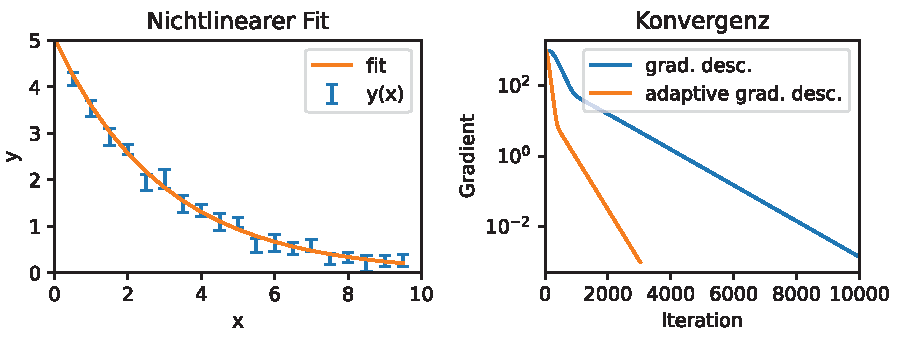
\includegraphics[width=0.8\textwidth]{Figures/nonlinear_fitting_image.pdf}
        \caption{Beispiel zum nichtlinearen Fitten. \textbf{Links:} Nichtlinearer Fit einer Exponentialfunktion zu fehlerbehafteten Daten. \textbf{Rechts:} Konvergenz des Gradientenverfahrens und des Newton-Verfahrens.  }
        \label{fig:nonlinearFit}
\end{figure} 

\subsection{Qualität des Fits}
\label{subsec:vl9-3}

Mit diesen Methoden können wir ausgehend von den Anfangswerten für die Fit parameter ein Minimum der Kostenfunktion $S$ bestimmen. Ob dieses Minimum jedoch das Globale, oder ein lokales Minimum ist, ist nicht sicher. Wir könne das Ergebnis des Fits zusammen mit den Daten plotten um beurteilen zu können, ob die Daten gut beschrieben werden und ob nach unserer Vorstellung, das globale Minimum gefunden wurde.

Darüber hinaus, bietet es sich an die Residuen zu betrachten, um zu evaluieren, wie gut der Fit die Daten beschreibt. Dazu berechnen wir $\epsilon_i =y_i - f(x_i, \boldsymbol{\hat{a}})$ für den gesamten Datensatz um die Modellparameter $\boldsymbol{\hat{a}}$ und $S$ zu minimieren. Idealerweise sollten die Abweichungen $\epsilon_i$ der gemessenen Werte $y_i$ von der Fitfunktion $f(x_i, \boldsymbol{\hat{a}})$ nur durch zufällige (statistische), unkorrelierte Fehler zustande kommen. In diesem Fall beschreibt unser Modell die Daten gut und die Voraussetzungen für die Berechnung der Unsicherheiten der Fitparameter (siehe \cref{eq:vl8-30}) sind erfüllt.\\
Wenn die Residuen nicht zufällig und symmetrisch um die Null verteilt sind, sondern systematische Abweichungen und Korrelationen aufweisen, dann beschreibt das Modell die Daten nur unzureichend (Wobei hier kleine Abweichungen oft nicht vermieden werden können und in Kauf genommen werden müssen). Diese Abweichung kann durch systematische Fehler in der Messung hervorgerufen werden, die durch eine Optimierung des Messaufbaus bzw. durch Anpassung des Modells reduziert oder vermieden werden können. Andererseits kann auch das physikalische Modell nicht das richtige sein, um den gemessenen Effekt zu beschreiben. Dann muss das Modell erweitert, oder ein anderes Modell gewählt werden. Es ist auf jeden Fall zu beachten, dass die Unsicherheiten der Fitparameter unzuverlässig sind wenn die Residuen zu starke Korrelationen aufweisen.


\subsection{Zusammenfassung}
\label{subsec:vl9-4}

\begin{itemize}
    \setlength\itemsep{0em}
        \item Wir können für jede Funktion die Kostenfunktion $S$ (die Summe der Abstandsquadrate) definieren.
        \item Minimieren von $S$ erlaubt uns die Funktionsparameter zu finden für die die Funktion die Daten am besten beschreibt.
        \item Dazu folgen wir iterativ dem Gradienten von $S$ zum Minimum.
        \item Die Unsicherheit der Fitparameter können wir mit Hilfe der Hesse-Matrix berechnen.
        \item Die meisten Datenanalysewerkzeuge stellen effiziente und zuverlässige Implementationen dieser Methoden zu Verfügung, in Python z.B. ``lmfit''.
\end{itemize}


\newpage

\begin{tcolorbox}[enhanced,width=6in,
    fontupper=\small,drop fuzzy shadow southwest,
    colframe=black!50!black,colback=black!5]
\textbf{Verständnisfragen:} \\
\begin{enumerate}
\item[1] Was ist die Likelihood Funktion?
\item[2] Warum ist die Likelihood Funktion keine Wahrscheinlichkeitsverteilung? 
\item[3] Warum wollen wir die Likelihood Funktion maximieren? 
\item[4] Welchen Sinn hat die Log-Likelihood Funktion? 
\item[5] Was bedeuten die Residuen im Kontext eines Fit mit einer Ausgleichsgerade? 
\item[6] Was ist die Normalmatrix? 
\item[7] Warum funktioniert das invertieren der Normalmatrix nicht bei nichtlinearen Fitten? 
\item[8] Wie berechnet man die Unsicherheit der Fitparameter beim Nichtlinearen Fitten? 
\end{enumerate}
\end{tcolorbox}

\begin{tcolorbox}[enhanced,width=6in,
    fontupper=\small,drop fuzzy shadow southwest,
    colframe=black!50!black,colback=black!5]
\textbf{Antworten:} \\
\begin{enumerate}
\item[1] Die Likelihood Funktion gibt ein relatives Maß wie gut ein Modell mit Parametern $a_i$ zu bekannten Datenpunkten $x_i$ passt.
\item[2] Die Likelihood Funktion ist keine Wahrscheinlichkeiteverteilung, weil sie nicht normiert ist. 
\item[3] Die Parameter $a_i$, die die Likelihood Funktion maximieren, beschreiben die gemessenen Daten am besten, sodass wir ein aussagekräftigeres Modell erhalten. 
\item[4] Da die Likelihood Funktion nicht normiert ist, sind für uns nur relative Änderungen relevant. Oft erstrecken sich die Werte der Likelihood Funktion über viele Größenordnungen, sodass der Logarithmus der Likelihood Funktion ihre numerischen Werte besser vergleichbar macht. Zusätzlich können über die Log-Likelihood Funktion verschiedene Ausdrücke wie der Erwartungswert und die Varianz hergeleitet werden. 
\item[5] Die Residuen beim Fit mit einer Ausgleichsgerade sind die Abstandsquadrate der Datenpunkte vom Fit Modell. Die gewichtete Summe der Residuen gibt an wie weit unsere Gerade von der optimalen Auslgeichsgerade entfernt ist.  
\item[6] Die Normalmatrix ist die Matrixform des linearen Gleichungssystems das man erhält wenn man die Summe der Residuen minimiert. Invertieren der Normalmatrix lässt uns aus den gemessenen Datenpunkten die Parameter eines Polynoms berechnen, das diese Datenpunkte optimal beschreibt. 
\item[7] Beim Ableiten der Summe der Residuen einer nichtlinearen Funktion ergibt sich nicht unbedingt ein lineares Gleichungssystem welches wir als Normalmatrix schreiben könnten. Daher müssen wir die Summe der Residuen iterativ minimieren.  
\item[8] Die Unsicherheiten der Parameter bei einem nichtlinearen Fit können abgeschätzt werden, indem man die nichtlineare Funktion entwickelt und dann behandelt wie eine lineare Funktion. 
\end{enumerate}
\end{tcolorbox}
\chapter{Machine Learning}
\begin{center}
\begin{tcolorbox}[enhanced,width=6in,center upper,
    fontupper=\large,drop fuzzy shadow southwest,
    colframe=blue!50!black,colback=blue!10]
Für dieses Unterkapitel ist ein Jupyter-Notebook verfügbar. Siehe \gitresource{Machine Learning.ipynb}  
\end{tcolorbox}
\end{center}

\section{Grundzüge von Machine Learning}
Das Ziel von Machine Learning (ML) ist die Reproduktion von biologischem Lernverhalten in Computern. 
Ein Beispiel aus der Objekt-Klassifizierung: Menschen können schnell eine Lampe von einem Buch unterscheiden, obwohl es sehr viele verschiedene Lampen und Bücher gibt. 
Es ist allerdings schwierig, eine formelle Definition von \textit{Lampe} zu geben und somit Algorithmen zu entwerfen. 
Wir Menschen treffen solche Entscheidungen nicht mithilfe von solchen Definitionen, sondern wir benutzen unsere vorherigen Erfahrungen. Eine Lampe ist eine Lampe, weil es unsere vorherigen Erfahrungen mit Lampen widerspiegelt.\\

Da Computer keine Erfahrungen sammeln wie Menschen, brauchen wir eine Methode, um Computern etwas beizubringen. 
Wir müssen folgendes für den Computer bereitstellen:
\begin{enumerate}
    \item \textbf{Datensatz: } z.B. Bilder von Lampen
    \item \textbf{Modell: } in der Biologie ist dies das Gehirn
    \item \textbf{Verlustfunktion: } ein Mass dafür wie falsch die Aussagen sind.
\end{enumerate}
Wenn wir diese haben, können wir den Computer trainieren und dann validieren. 

\subsection{Datensatz}
Ein Datensatz ist eine Tabelle mit beliebig vielen Merkmalen und einem Klassifizierungslabel (\textit{class label}). Die Merkmale können Antworten zu ja-nein-Fragen oder aber auch Zahlen sein. Die Merkmale für eine Lampe können zum Beispiel die folgenden sein:
\begin{itemize}
    \item Ist es hell?
    \item Kann man es aus- und einschalten?
    \item Verwendet es Elektrizität?
\end{itemize}
Das class label ist dann: Ist es eine Lampe?
Wir werden ein Modell so trainieren, dass es aus den Merkmale das class label vorhersagen kann. 

\subsection{Modell}
Ein Modell ist eine Menge von möglichen Algorithmen, die die Merkmale als Argument nehmen und ein class label als Antwort zurückgeben. Wir beschriften diese Menge oft $\mathcal{H}$. Beispiele sind Entscheidungsbäume oder Neuronale Netze bestimmter Struktur. 

\subsection{Verlustfunktion}
Eine Verlustfunktion $L(D,f)$ ist eine Funktion, die einen Datensatz D und eine $f \in \mathcal{H}$ als Argument nimmt und die Fehlerrate der $f$ in $D$ quantifiziert. Für Entscheidungsbäume wäre der Anteil von falschen Klassifizierungen eine mögliche Verlustfunktion. Es gibt keine allgemeine Verlustfunktion, sondern man muss eine für das Modell $\mathcal{H}$ auswählen.

\subsection{Training}
Das Training minimiert die Verlustfunktion anhand von Trainingsdaten. Wie man dies spezifisch schafft, ist abhängig von dem Modell und der Verlustfunktion. Es ist oft in Python Packages für verschiedene Modelle implementiert.

\subsection{Validierung}
Für Validierung verwenden wir einen anderen Datensatz $D'$ (also nicht den Trainingsdatensatz und überprüfen, dass die von Training ausgewählte $f^* \in \mathcal{H}$ auch für andere Datensätze funktioniert. Es kann sein, dass unser Modell nur den Datensatz D auswendig gelernt hat und keine Aussagen über andere Datensätze machen kann. Wie müssen deshalb sicherstellen, dass dies nicht der Fall ist.
\section{Ausgewählte Modelle}\label{ml:modelle}
\subsection{Entscheidungsbäume}
Entscheidungsbäume sind eine einfache Art, Datensätze mit binären Merkmalen zu klassifizieren. Sie bestehen aus einer Wurzel, Knoten und Blättern. 
Wurzeln und Knoten sind immer mit zwei Knoten oder Blättern verbunden und fragen immer nach einem bestimmten Merkmal in dem Datensatz. Abhängig von der Antwort wird man nach links oder nach rechts verwiesen. Die Konvention ist, dass eine ja-Antwort nach rechts und eine nein-Antwort nach links führt. Blätter sind die Enden vom Baum und geben  an, welches class label zu dieser spezifischen Kombination von Merkmalen gehört. Am besten stellt man sie grafisch dar ( z. B. Abb. \ref{fig:ml-baum}).\\

\begin{figure}[h]
    \centering
    \includegraphics[scale=0.4]{Figures/ML-Baum.png}
    \caption{Muster-Entscheidungsbaum aus der Vorlesung.}
    \label{fig:ml-baum}
\end{figure}

Da Bäume theoretisch unendlich lang sein könnten, setzt man vorher eine Tiefe fest. Die Tiefe ist einfach die maximal erlaubte Anzahl von hintereinander gelegten Knoten. Wie man eine gute Tiefe wählen kann, werden wir später sehen.\\

Eine praktische Verlustfunktion für Entscheidungsbäume ist:
\begin{equation}
    L(D,f) = \frac{\mathrm{Anzahl ~falsch ~klassifizierte ~Elemente ~in ~D}}{\mathrm{Anzahl ~Elemente ~in ~D}}~.
\end{equation}
\subsection{Lineare Regression}
Lineare Regression verwenden wir, wenn sowohl die Merkmale als auch die class labels  Zahlen sind. 
Für $n$ Merkmale ist unser Modell die Menge von allen $n$-dimensionalen Linearformen. 
Die Vorhergesagte class label $y$ ist dann die Linearform angewendet auf die Merkmale.

\begin{equation}
    \mathcal{H} = \left\{ y=f(x_1,...,x_n) = \sum_{i=1}^n w_ix_i ~~|~w_1,..,w_n \in \mathbb{R}\right\}
\end{equation}

Die Verlustfunktion (auch \textit{Mean Squared Error} genannt) ist dann:
\begin{equation}
    L(D, f) = \mathrm{MSE}(D,f) = \frac{1}{m} \sum_{i=1}^m (f(x_{1,i},...,x_{n,i}) - y_i)^2
\end{equation}
wobei $m$ die Anzahl von Zeilen in $D$ und $(x_{1,i},...,x_{n,i},y_i)$ die Zeilen des Datensatzes sind.\\

Um einzuschätzen, wie gut die Regression ist, bestimmen wir den \textbf{R2}-Wert eines Schätzers $f \in \mathcal{H}$. Wir definieren zuerst ein $f_0 = \frac{1}{n}\sum y_i$, der immer den Mittelwert der Trainingsdaten zurückgibt. Die R2-Score ist dann:
\begin{equation}
    R2(D,f) = 1 - \frac{\mathrm{MSE}(D,f)}{\mathrm{MSE}(D,f_0)}
\end{equation}


Ein negativer R2-Wert bedeutet, dass der Schätzer schlechter ist, als einfach immer den Mittelwert zurückzugeben. Je näher der R2-Wert an 1 ist, desto besser ist f. 

\subsection{Logistische Regression}
Logistische Regression wird verwendet, wenn man ein binäres class label und skalare Merkmale hat. Eine grafische Darstellung ist das Teilen des kartesischen Koordinatenraums in zwei Gebiete (siehe Abb. \ref{fig:ml-div}).

\begin{figure}[h]
    \centering
    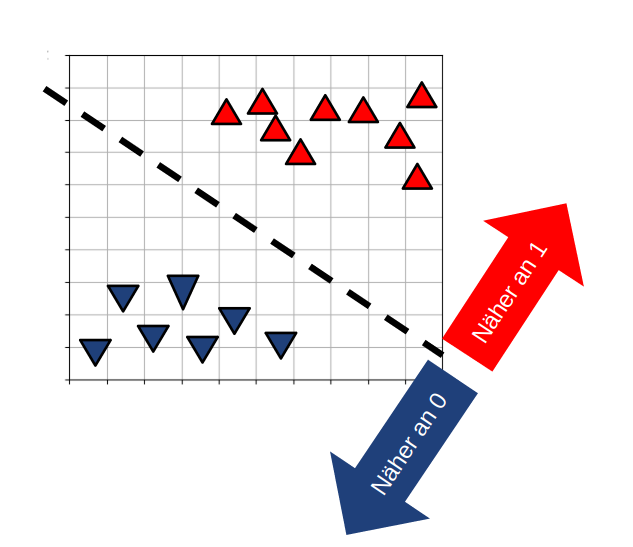
\includegraphics[scale=0.27]{Figures/ML-divided space.png}
    \caption{Beispiel für logistische Regression aus der Vorlesung.}
    \label{fig:ml-div}
\end{figure}

Dafür verwenden wir das Modell:
\begin{equation}
        \mathcal{H} = \left\{ y=f(x_1,...,x_n) = \sigma (w_0 + w_1*x_1 + ... + w_n*x_n) ~~|~w_0,..,w_n \in \mathbb{R}\right\}
\end{equation}
wobei  $\sigma$ die Sigmoidfunktion $\sigma: \mathbb{R} \to (0,1)$ ist. \footnote{Die Verlustfunktionen sind mathematische Normen für den Funktionenraum $L^2$ (nicht klasurrelevant, für mehr Information MMP I)}

\section{Einschub: Under- und Overfitting}
In diesem Einschub werden wir Entscheidungsbäume näher betrachten. Wir möchten besonders den Einfluss von \textit{Tiefe} auf dem Erfolg des Modells verstehen.\\ 

Es gibt zwei mögliche Fälle:
\begin{enumerate}
    \item \textbf{Underfit: } Die Tiefe war zu klein, sodass das Modell nicht genügend lernen konnte.
    \item \textbf{Overfit: } Die Tiefe war zu gross. Das Modell hat den Datensatz auswendig gelernt. Wir haben nur den Datensatz auf dem Format von einem binären Baum umgeschrieben.
\end{enumerate}
Das ideale Modell hat eine Tiefe, die weder zu groß noch zu klein ist. Die einfachste Methode, diese Tiefe zu finden, ist, verschiedene Tiefen auszuprobieren. 

Sei $D$ der Datensatz, $\mathcal{H}_n$ Entscheidungsbäume der Tiefe $n$, und $f_{n,D^*} \in \mathcal{H}_n$ der Baum, der eine Verlustfunktion auf $D^*$ minimiert. Mit den folgenden Methoden kann man eine gute Tiefe finden.
\subsection{Crossvalidation} \label{ML-Crossval}
\begin{enumerate}
    \item Teile D in ein \textit{training} Dataset $D^*$ und ein \textit{validation} Dataset $D'$. Oft ist das Training-Dataset länger. 
    \item Wähle Tiefen $t_1,...t_i$, die untersucht werden sollen.
    \item Finde $f_{t_1,D^*},...,f_{t_i,D^*}$ durch das Training und berechne $L(D',f_{t_1,D^*}),...,L(D',f_{t_i,D^*})$
    \item  Die Tiefe mit dem minimalen Verlustwert in 3. ist die optimale Tiefe.

\end{enumerate}
\subsection{k-Fold Crossvalidation}
\begin{enumerate}
    \item Teile $D$ in $k$ gleichlange Teile. Wir nennen diese $D_1,...,D_k$. 
    \item Für jedes $D_i$ führe crossvalidation \ref{ML-Crossval} mit $D_i$ als \textit{validation} Dataset und Rest von D als \textit{training} Dataset aus. 
    \item Die Tiefe, die am häufigsten den minimalen Verlustwert hatte, ist die optimale Tiefe. 
\end{enumerate}

\section{Neuronale Netze}
\textit{Neuronale Netze} bezeichnet ein Modell, das direkt von  biologischen Strukturen inspiriert ist. Ein Neuron im ML-Sinne  besteht aus gewichteten Eingängen und einem Ausgang. Die Neuronen sind in neuronalen Netzen in Schichten organisiert. Die Ausgänge von den Neuronen in einer Schicht sind die Eingänge der Neuronen in nächster Schicht.\\
\begin{figure}[h]
    \centering
    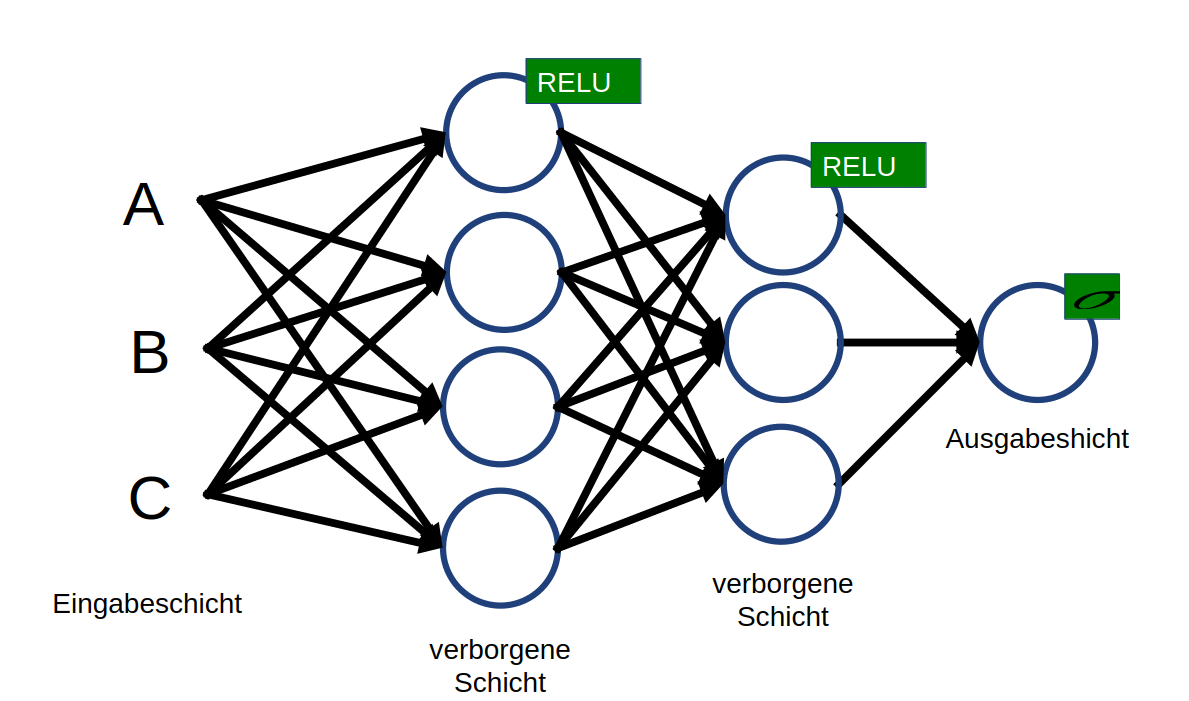
\includegraphics[scale=0.3]{Figures/ML-NNetz.png}
    \caption{Ein Beispiel für ein neuronales Netz. }
\end{figure}

Neuronen sind mathematisch folgenderweise konstruiert: 
\begin{equation}
    f(x_1,...,x_n) = a(c + w_1 x_1 + ... + w_n x_n)
\end{equation}
wobei $a$ eine Aktivierungsfunktion $a: \mathbb{R} \to \mathbb{R}$ ist. Häufig verwendete Aktivierungsfunktionen sind  in Tabelle \ref{ML:aktivierungsfunktionen} zu sehen. Die RELU wird heutzutage am meisten verwendet.\\

 
\begin{table}[h]
\centering
\begin{tabular}{lllll}
\cline{1-2}
\multicolumn{1}{|l|}{RELU}   & \multicolumn{1}{l|}{f(x) = max(0,x)}              &  &  &  \\ \cline{1-2}
\multicolumn{1}{|l|}{$\sigma$} & \multicolumn{1}{l|}{$f(x) = \frac{1}{1+e^{-x}}$}    &  &  &  \\ \cline{1-2}
\multicolumn{1}{|l|}{TANH}   & \multicolumn{1}{l|}{$f(x) = \frac{2}{1+e^{-2x}}-1$} &  &  &  \\ \cline{1-2}
                             &                                                   &  &  & 
\end{tabular}
\caption{Häufig verwendete Aktivierungsfunktionen.}
\label{ML:aktivierungsfunktionen}
\end{table}

Während des Trainings sind die Gewichte $c, w_1,...,w_n$ für jedes Neuron zu optimieren. Die Struktur von den Neuronen ist vorher zu finden.

\subsection{Convolutional Neural Networks}
Das Hauptziel von CNNs ist Bilderkennung. Wir möchten immer noch Objekte voneinander unterscheiden, aber statt skalarer Merkmale möchten wir jetzt Bilder betrachten. Als erste Idee könnten wir jeden Pixel als Eingang zu einem neuronalen Netz nehmen und ein riesiges Netzwerk verwenden, um die Klassifikation durchzuführen. Aber dafür bräuchten wir zu viele Neuronen. Stattdessen verwenden wir \textit{convolution} \footnote{Convolution ist hier nicht im Sinne von \textit{Complex} (convoluted), sondern im Sinne von \textit{Faltung} zu verstehen. }, um die Bilder zu vereinfachen. Für Faltung betrachten wir Bilder als Matrizen. Sei $E \in \mathbb{R}^{nxn}$ die zu faltende Matrix und $F \in {0,1}^{2x2}$ die Faltungsmatrix. Der Ausgang ist $A \in \mathbb{R}^{n-1xn-1}$. \footnote{Falls $n$ kein ganzzahliges Mehrfaches von der Größe von $F$ ist, dann vernachlässigt man genügend der letzten Zeilen und Spalten von $E$.}
\begin{equation}
    A_{i,j} = E_{i,j}F_{1,1} + E_{i+1,j}F_{2,1} + E_{i,j+1}F_{1,2} +E_{i+1,j+1}F_{2,2}     
\end{equation}
Man stellt dies am besten grafisch dar: Man legt die Faltungsmatrix auf jeden 2x2 Block in $E$, multipliziert die Einträge, die aufeinander liegen, summiert die Ergebnisse, und notiert die Summe auf einer neuen Matrix für jeden 2x2 Block in $E$. \\

Man kann noch einen Filter (Aktivierungsfunktion) auf das Ergebnisse anwenden. Zum Beispiel:
\begin{equation}
        A_{i,j} = RELU( E_{i,j}F_{1,1} + E_{i+1,j}F_{2,1} + E_{i,j+1}F_{1,2} +E_{i+1,j+1}F_{2,2} )
\end{equation}

Eine weitere Methode, die für CNN verwendet wird, ist \textit{Pooling}. Es wird ähnlich wie Faltung angewendet, aber es keine lineare Funktion, sondern \textit{max} oder \textit{min}:
\begin{equation}
    A_{i,j} = \mathrm{max}\{E_{i,j};E_{i+1,j};E_{i,j+1};E_{i+1,j+1}\}
\end{equation}

Eine geschickte Wahl von Faltungsschichten führt nicht nur zu einer Reduktion der Bilddimension, sondern auch zu Hervorhebung von Merkmalen (Kanten, Ecken etc.) des gesuchten Objekts (siehe Abb. \ref{fig:ml-conv}. Man kann die "gefalteten" Bilder dann mithilfe eines neuronalen Netzes klassifizieren.

\begin{figure}[h]
    \centering
    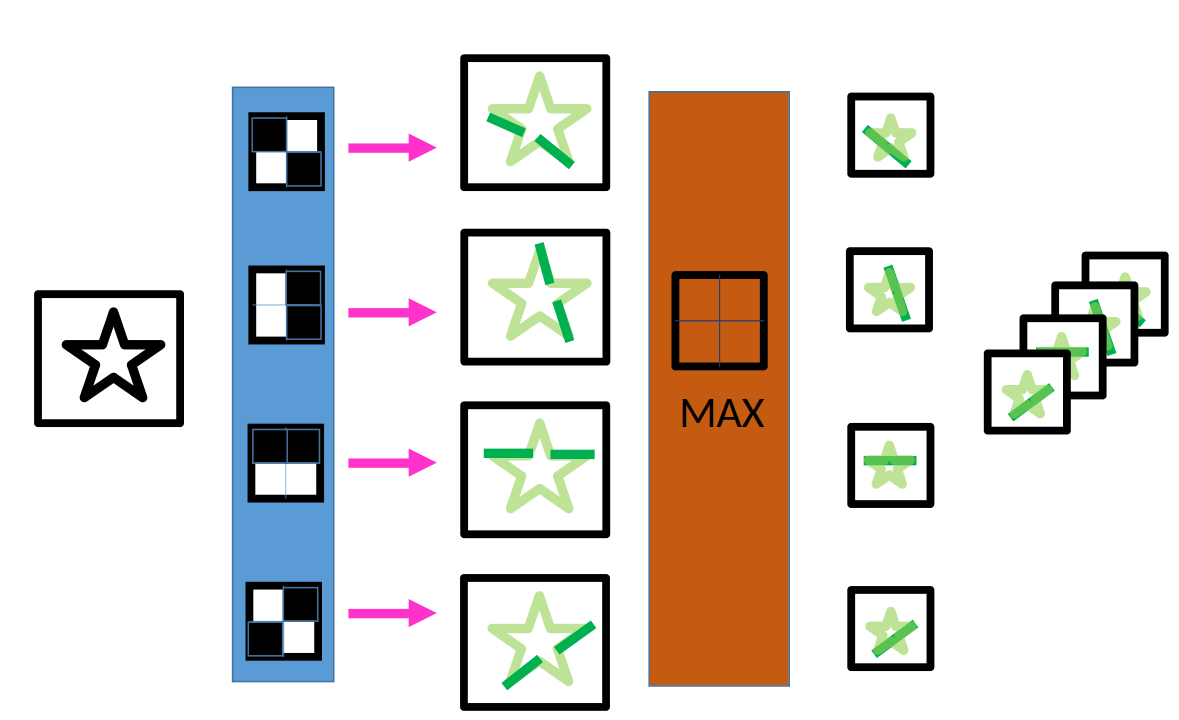
\includegraphics[scale= 0.3]{Figures/ML-conv.png}
    \caption{Hier werden die Kanten von einem Stern mit einem CNN hervorgehoben. Die nachfolgenden neuronalen Netze können dann aus den Kanten entscheiden, ob es einen Stern ist.}
    \label{fig:ml-conv}
\end{figure}
\subsection{Andere Architekturen}
\subsubsection{Autoencoder}
Ein Autoencoder besteht aus einem Encoder und einem Decoder. Der Encoder überführt die Eingangsinformation (Bild oder Data) in einen mehrdimensionalen Raum (auch Code Space genannt). Der Decoder ist die umgekehrte Operation. Die Idee ist, dass ähnliche Eingänge näher zu einander im Code Space abgebildet werden. Dann können wir mithilfe von Clustering die Daten klassifizieren. Ein Beispiel ist Schrifterkennung. Bilder von Schriftzeichen werden mithilfe von einem Encoder auf dem Code Space abgebildet. Dann können wir aus der Position im Code Space erkennen, welches Schriftzeichen es war.\\

Der Encoder und Decoder sind neuronale Netze, die auch trainiert werden müssen. Die Layer sind Sanduhr artig, dies führt dazu, dass nur die wichtigste Information im Code Space abgebildet wird. Was diese Information (bzw. was die Achsen von Code Space) bedeuten ist a priori unbekannt. Die Verlustfunktion für Training ist:
\begin{equation}
    L(D, Enc,Dec) = \sum_{x\in D} || x -Dec(Enc(x))||^2
\end{equation}

\subsection{Generative Adversarial Networks (GAN)}
GANs sind dafür geeignet, um Bilder zu generieren oder zu verändern. Ein GAN hat einen Generator, der Bilder generieren kann und einen Diskriminator, der Bilder beurteilen kann. Der Diskriminator versucht die Bilder vom Generator von echten Bildern unterscheiden zu können. Der Generator versucht Bilder, die vom Diskriminator als ``echt`` gesehen werden, zu generieren.

\section{Kodierung kategorischer Daten}
Wie wir gesehen haben, arbeiten alle bisherige Modelle auf numerischen Daten (entweder {0,1} oder $\mathbb{R}$), aber im reellen Leben sind Daten oft nicht numerisch, sondern kategorisch \footnote{z.B Gender wird oft mit männlich, weiblich oder divers bezeichnet. Diese lassen sich aber nicht natürlicherweise mit Zahlen ausdrücken. }. Deshalb müssen wir uns bewusst eine Codierung auswählen. In dem folgenden Paragrafen betrachten wir verschiedene Methoden anhand des Titanik-Dataset (siehe Abbildung \ref{fig:titanik-dataset}).

\begin{figure}
    \centering
    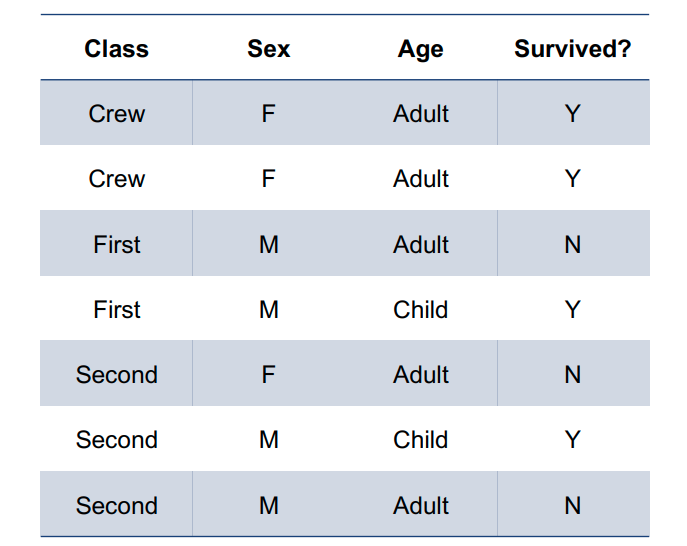
\includegraphics[scale=0.4]{Figures/Ml-Titanik-Dataset.png}
    \caption{Auszug des Titanik Datasets. }
    \label{fig:titanik-dataset}
\end{figure}
\subsection{Ordinal Encoding}
Dies ist die einfachste Methode. Mögliche Kategorien jedes Merkmals werden mit arbiträren ganzen Zahlen bezeichnet. Zum Beispiel im Titanik-Dataset können wir für das Merkmal \textit{class} Crew mit 1, First mit 2 und Second mit 3 bezeichnen. Obwohl wir die Zahlen willkürlich gewählt haben, haben wir plötzlich Crew näher mit First als mit Second platziert. Das kann  in der Auswertung nachteilig sein.

\subsection{Mean Encoding}
Hier bezeichnen wir jede Kategorie mit einem Mean, der mit Hilfe von dem \textit{class label} generiert wird. In unserem Fall können wir dieses Mean als Überlebenschance nehmen. Für \textit{Age} Merkmal bezeichnen wir \textit{Kind} mit 1, denn jedes Kind hat überlebt, und \textit{Adult} mit 0.4, denn 40 \% der Erwachsene haben überlebt. Nachteil ist, dass wir plötzlich Information aus dem \textit{class label} in die Merkmale übertragen haben. Dies kann zu Overfitting führen.

\subsection{One-Hot Encoding}
Für diese Methode machen wir aus einem Merkmal mit $n$ Kategorien $n$ Merkmale, d.h. z. B. für das Merkmal \textit{class}: Es gibt jetzt drei Merkmale mit Werten {0,1}. Diese sind ''Ist Crew?'', ''Ist First?'' und ''Ist Second?''. Dadurch haben wir keinen der Nachteile der vorherigen Methoden, aber unser Datensatz ist \textit{viel}\footnote{Der Titanik-Datensatz hat nach One-Hot Encoding ca. 2 mal mehr Merkmale.} größer geworden. 


\section{Clustering \& K-Means-Methode}
Wir möchten unsere Daten mit skalaren Merkmalen (z.B. Helligkeit und Größe für Sterne) gemäß ihrer Entfernung zueinander in Clusters (Bündel) sammeln. Die k-Means-Methode dient dazu, die geeigneten Bündel zu finden. Unser Modell ist
\begin{equation}
     \mathcal{H} = \left\{ (\theta_1,...,\theta_k,c) | \theta_1,...,\theta_k \in \mathbb{R}^d \land c : \mathbb{R}^d \to \{1,...,k\} \right\}
\end{equation}
wobei wir k Bündel mit Mittelpunkt (auch Zentroid benannt) $\theta$ und die Zuweisungsfunktion $c$ betrachten. Die Funktion $c$ gibt für jeden Punkt in $\mathbb{R}^d$ an, zu welchem Bündel dieser Punkt gehört. Zu bemerken ist, dass dies kein neuronales Netz ist. Die Verlustfunktion ist so gedacht, dass der Abstand der Punkten zu ihrem zugewiesenen Cluster-Mittelpunkt bestraft wird. Wir formalisieren dies wie folgt:\\

$D \subseteq \mathbb{R}^d$ sind die gegebenen Punkte,  $\{\theta_1,...,\theta_k\} \subseteq \mathbb{R}^d$ die Cluster-Mittelpunkte, $c$ die Zuwesiungsfunktionen. Dann ist die Verlustfunktion: 
\begin{equation}
    \mathcal{L}(D,\theta_1,...,\theta_k,c) = \sum_{x \in D} || x - \theta_{c(x)}||^2 
\end{equation}
Bemerkung: $\theta_{c(x)}$ ist der  $x$ zugewiesene Mittelpunkt.\\

Für das Training verwenden den folgenden Algorithmus:

\begin{itemize}
    \item \textbf{Gegeben: } $D \in \mathbb{R}^d$
    \item \textbf{Initialisierung: } wähle $\theta_1,...,\theta_k$ zufällig. 
    \item \textbf{Zuweisung aktualisieren: } wir setzen $c(x) = argmin_{j \leq k} || x -\theta_j||$. Dies bedeutet, dass jedem Punkt der nächstgelegene Cluster-Mittelpunkt zugewiesen wird.
    \item \textbf{Cluster-Mittelpunkte aktualisieren: } Sei $S_j = \left\{ x \in D | c(x) = j\right\}$ die Menge der Punkte in Cluster $j$. $\forall j \leq k$ setze $\theta_j = \frac{1}{|S_j|} \sum_{x \in S_j} x$. Somit haben wir alle Cluster-Mittelpunkte auf den wirklichen Mittelpunkt des Clusters gesetzt.
    \item Führe die Aktualisierung-Schritte immer wieder durch, bis die Clusters sich nicht mehr ändern. 
\end{itemize}
\begin{figure}
    \centering
    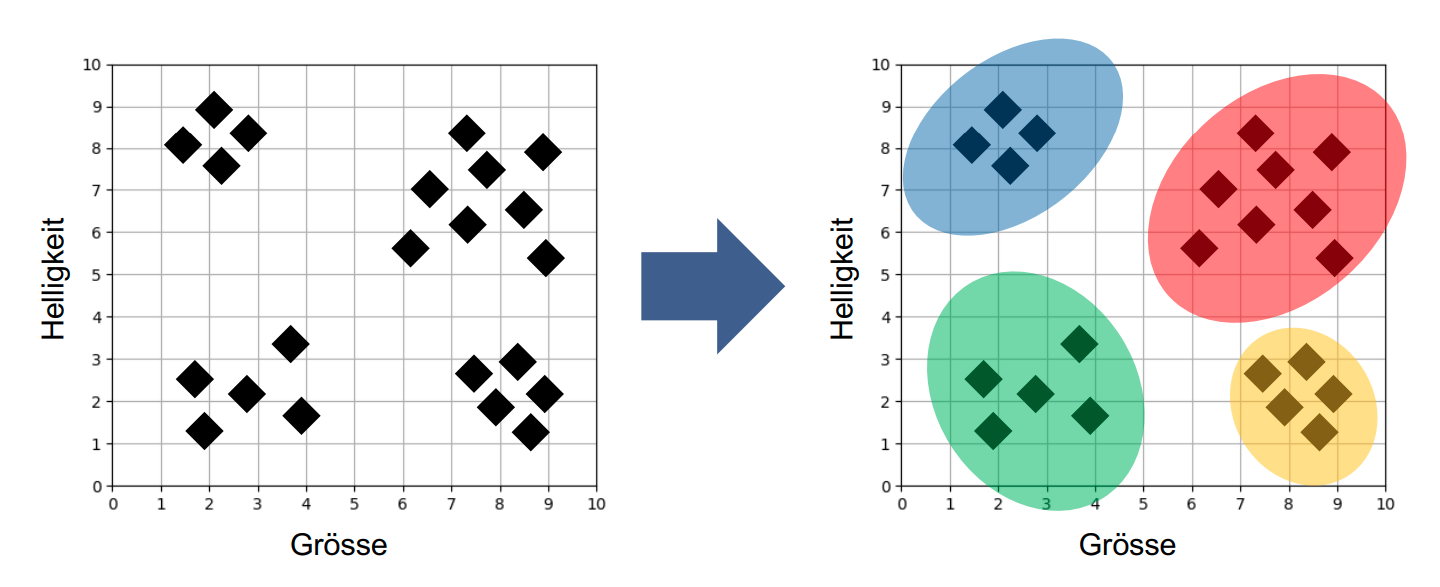
\includegraphics[scale=0.3]{Figures/ML-Clustering.png}
    \caption{Graphische Vorstellung des Clustering.}
\end{figure}
\subsection{Overfitting}
Wenn wir $k$ zu gross wählen (z.B  $k \geq |D|$), dann ist die beste Zuordnung immer einen Punkt pro Cluster. Wir können dies  nicht mit Cross-Validation (siehe \ref{ML-Crossval}) bemerken, denn $\mathcal{L}$ strebt gegen 0 für $k$ gegen $|D|$. Wenn wir mit Cross-Validation Overfitting verhindern wollen, dann müssen wir die Verlustfunktion so verändern, sodass sie auch große k bestraft. Wir verwenden mit $\lambda > 0$:
\begin{equation}
    L = \mathcal{L} + \lambda e^k
\end{equation}
Jetzt können wir Cross-Validation verwenden, um die optimale Anzahl Clusters zu finden. 

\section{Principal Component Analysis (PCA)}
Als Letztes betrachten wir die PCA, was dafür gedacht ist, die Dimension (Anzahl Merkmale) ohne große Verluste von Information zu reduzieren. Dies ist nützlich, weil so unsere anderen Modelle schneller und korrekter funktionieren, wobei besonders wichtig ist, dass sie korrekter werden. Mit einer hohen Anzahl von Merkmalen wird der Suchraum $\mathbb{H}$ größer und es kann sein, dass wir nicht die perfekte Lösung finden.

Formell ist PCA eine Methode unseren Datensatz $\{x_1,...,x_n\} \subseteq \mathbb{R}^D$\footnote{Die $x_i$'s sind die Zeilen des Datensatzes und  $D$ ist die Anzahl von Merkmalen. } auf einem reduzierten Datensatz $\{t_1,...,t_n\} \subseteq \mathbb{R}^d$ abzubilden. Aus Lineare Algebra Perspektive ist die PCA eine Abbildung auf einen Unterraum. Wir möchten allerdings  so viel Information wie möglich behalten. Die Abbildung wird $\forall i \leq n$ folgenderweise definiert:
\begin{equation}
    t_i = (x_i \cdot w_1 ,... x_i \cdot w_d)^T
\end{equation}
wobei $\{w_1,...,w_d\} \subseteq \mathbb{R}^D$ die Gewichtsvektoren sind. 

\textbf{\textit{Fall 1: d=1}}\\


In diesem Fall suchen wir nur die $w_1$, sodass $t_i = (x_i \cdot w_1) \in \mathbb{R}$ die  Streuung  $\sum t_i^2$ maximiert. Sei \textbf{X} die $n\times D$ Matrix, die in jeder Zeile ein Element aus dem Datensatz hat.

\begin{equation}
    X = \begin{pmatrix}
        - ~x_1~ -\\
        - ~ x_2 ~ - \\
        .\\.\\.\\
        -~x_n~-
        \end{pmatrix}\\
\end{equation}
Dann können wir $w_1$ mit Hilfe folgender Gleichung finden: 
\begin{equation}
    w_1 = argmax_{||w|| = 1}\left\{ \sum_i^n (x_i\cdot w_n)^2 \right\}= argmax_{||w|| = 1} \left\{||\textbf{X}w||^2\right\}
\end{equation}
Die Ausdruck $||\textbf{X}w||^2$ wird maximal, wenn $w$ der Eigenvektor $u_1^*$ zum größten Eigenwert $\lambda_1^*$ ist. Dies kann mit Methoden aus der linearen Algebra finden. \\

\textbf{\textit{Fall 2: $d \geq 1$}}\\

In diesem Fall suchen wir $d$ Gewichtsvektoren. $w_1$ ist wieder wie in Fall 1 zu finden, für die $w_2$ subtrahieren wir die Projektion von $x$ auf den Unterraum \textit{Spann}{$[w_1]$} von $x$ für jedes $x \in X $ also:
\begin{equation}
    X_1 = \{x - proj_{u_1}^* x | x \in x\} = \{x - (x \cdot u_1^*)u_1^* | x \in x\}
    \label{eq_ml_proj_set}
\end{equation}
Dann können wir noch einmal die Methode von Fall 1 (aber jetzt mit $X_2$ als Datensatz) anwenden, um $w_2$ zu bestimmen. Folglich können wir mit mehrmaligem Anwenden $(w_1,...,w_d)$ bestimmen. Formell geschrieben:

\begin{align}
    \textbf{X}_k &= \textbf{X} - \sum_{s=1}^{k-1} \textbf{X}w_s w_s^T\\ \label{eq_ml_mat_proj}
    w_k &=  argmax_{||w|| = 1} \left\{||\textbf{X}_k w||^2\right\}
\end{align}
Die Gleichung \ref{eq_ml_mat_proj} ist äquivalent zu mehrmaligen Anwenden von Gleichung \ref{eq_ml_proj_set}.

\setcounter{chapter}{0} 
\renewcommand{\thechapter}{\Alph{chapter}}

\chapter{Anhang}
\label{chap:anhang}

\section*{SI-Präfixe}
\begin{table}[ht]
\centering
\begin{tabular}{cccr}
\hline
\textbf{Präfix} & \textbf{Symbol} & \textbf{Potenzdarstellung} & \textbf{Dezimaldarstellung} \\
\hline
Yotta & Y & $10^{24}$ & 1'000'000'000'000'000'000'000'000 \\
Zetta & Z & $10^{21}$ & 1'000'000'000'000'000'000'000 \\
Exa & E & $10^{18}$ & 1'000'000'000'000'000'000 \\
Peta & P & $10^{15}$ & 1'000'000'000'000 \\
Tera & T & $10^{12}$ & 1'000'000'000 \\
Giga & G & $10^{9}$ & 1'000'000'000 \\
Mega & M & $10^{6}$ & 1'000'000 \\
Kilo & k & $10^{3}$ & 1'000 \\
Hekto & h & $10^{2}$ & 100 \\
\hline
\hline
Dezi & d & $10^{-1}$ & 0.1 \\
Centi & c & $10^{-2}$ & 0.01 \\
Milli & m & $10^{-3}$ & 0.001 \\
Micro & $\mathrm{\mu}$ & $10^{-6}$ & 0.000001 \\
Nano & n & $10^{-9}$ & 0.000000001 \\
Pico & p & $10^{-12}$ & 0.000000000001 \\
Femto & f & $10^{-15}$ & 0.000000000000001 \\
Atto & a & $10^{-18}$ & 0.000000000000000001 \\
Zepto & z & $10^{-21}$ & 0.000000000000000000001 \\
Yocto & y & $10^{-24}$ & 0.000000000000000000000001 \\
\hline
\end{tabular}
\end{table}

\renewcommand*{\arraystretch}{1.2}% default is 1
% \printnoidxglossary[type=main, title={Variablen}, sort=case]


\end{document}